% !TEX TS-program = xelatex
% Command for running this example (needs latexmkrc file):
%    latexmk -bibtex -pdf main.tex

%----------------------------------------------------------------------------------------------
% اگر قصد نوشتن پروژه کارشناسی را دارید، در خط زیر به جای msc، کلمه bsc و اگر قصد نوشتن رساله دکترا را دارید، کلمه phd را قرار دهید. کلیه تنظیمات لازم، به طور خودکار، اعمال می‌شود.

% اگر مایلید پایان‌نامه شما دورو باشد به جای oneside در خط زیر از twoside استفاده کنید.

% برای حاشیه‌نویسی و کم کردن صفحات ابتدایی، گزینه draft را وارد و برای نسخه نهایی آن را حذف کنید.

% برای استفاده از قلم‌های سری IR Series گزینه irfonts را وارد و برای استفاده از قلم‌های X Series 2 آن را حذف کنید.
\documentclass[
twoside
% ,openany
,msc
,irfonts
% ,draft
]{./kntu-thesis}

% فایل commands.tex را مطالعه کنید؛ چون دستورات مربوط به فراخوانی بسته‌ها، فونت و دستورات خاص در این فایل قرار دارد.
% در این فایل، دستورها و تنظیمات مورد نیاز، آورده شده است.
%-------------------------------------------------------------------------------------------------------------------
% دستوراتی که پوشه پیش‌فرض زیرفایل‌های tex را مشخص می‌کند.
%\makeatletter
%\def\input@path{{./tex/}}
%\makeatother
% در ورژن جدید زی‌پرشین برای تایپ متن‌های ریاضی، این سه بسته، حتماً باید فراخوانی شود
\usepackage{amsthm,amssymb,amsmath}
% بسته‌ای برای تنطیم حاشیه‌های بالا، پایین، چپ و راست صفحه
\usepackage[a4paper, top=40mm, bottom=40mm, outer=25mm, inner=35mm]{geometry}
% بسته‌‌ای برای ظاهر شدن شکل‌ها و تعیین آدرس تصاویر
\usepackage[final]{graphicx}
\graphicspath{{./img/}}



% بسته‌های مورد نیاز برای نوشتن کدها، رنگ‌آمیزی آنها و تعیین پوشهٔ کدها
%%man ezafe kardam
\usepackage{subfig}

\usepackage{diagbox}
\usepackage{multirow}
\usepackage{rotating}
\usepackage[final]{listings}
\usepackage[usenames,dvipsnames,svgnames,table]{xcolor}
\lstset{inputpath=./code/}
\usepackage[notransparent]{svg}
\usepackage[final]{pdfpages}
%\usepackage{tabularray}
\usepackage{booktabs, makecell, multirow, tabularx}
% بسته‌ای برای رسم کادر
\usepackage{framed} 
% بسته‌‌ای برای چاپ شدن خودکار تعداد صفحات در صفحه «معرفی پایان‌نامه»
\usepackage{lastpage}
% بسته‌ٔ لازم برای: ۱. تغییر شماره‌گذاری صفحات پیوست. ۲. تصحیح باگ آدرس وب حاوی '%' در مراجع
\usepackage{etoolbox}

%%%%%%%%%%%%%%%%%%%%%%%%%%%%%%%%%%%%
%%% دستورات وابسته به استیل مراجع:
%% اگر از استیل‌های natbib (plainnat-fa، asa-fa، chicago-fa) استفاده می‌کنید، خط زیر را فعال و بعدی‌اش را غیرفعال کنید.
%\usepackage{natbib}
%\newcommand{\citelatin}[1]{\cite{#1}\LTRfootnote{\citeauthor*{#1}}}
%\newcommand{\citeplatin}[1]{\citep{#1}\LTRfootnote{\citeauthor*{#1}}}


%% اگر از سایر استیل‌ها استفاده می‌کنید، خط بالا را غیرفعال و خط‌های زیر را فعال کنید.
\let\citep\cite
\let\citelatin\cite
\let\citeplatin\cite
%%%%%%%%%%%%
%% بررسی حالت پیش نویس
\usepackage{ifdraft}
\ifdraft
{%
	% بسته‌ٔ ایجاد لینک‌های رنگی با امکان جهش
	\usepackage[unicode=true,pagebackref=true,
colorlinks,linkcolor=blue,citecolor=blue,final]{hyperref}
	%\usepackage{todonotes}
	\usepackage[firstpage]{draftwatermark}
	\SetWatermarkText{\ \ \ \rl{پیش‌نویس}}
	\SetWatermarkScale{1.2}
}
{ 
	\usepackage[pagebackref=false]{hyperref}
	%\usepackage[disable]{todonotes} % final without TODOs
}

\usepackage[obeyDraft]{todonotes}
\setlength{\marginparwidth}{2cm}

%%%%%%%%%%%%
%%% تصحیح باگ: اگر در مراجع، آدرس وب حاوی '%' بوده و pagebackref فعال باشد، دستورات زیر باید بیایند:
%% برای استیل‌های natbib مثل plainnat-fa، asa-fa، chicago-fa
\makeatletter
\let\ORIG@BR@@lbibitem\BR@@lbibitem
\apptocmd\ORIG@BR@@lbibitem{\endgroup}{}{}
\def\BR@@lbibitem{\begingroup\catcode`\%=12 \ORIG@BR@@lbibitem}
\makeatother
%% برای سایر استیل‌ها
\makeatletter
\let\ORIG@BR@@bibitem\BR@@bibitem
\apptocmd\ORIG@BR@@bibitem{\endgroup}{}{}
\def\BR@@bibitem{\begingroup\catcode`\%=12 \ORIG@BR@@bibitem}
\makeatother
%%%%%%%%%%%%%%%%%%%%%%%%%%%%%%%%%%%%

% بسته‌ لازم برای تنظیم سربرگ‌ها
\usepackage{fancyhdr}
%\usepackage{enumitem}
\usepackage{setspace}
% بسته‌های لازم برای نوشتن الگوریتم
\usepackage{algorithm}
\usepackage{algorithmic}
% بسته‌های لازم برای رسم بهتر جداول
\usepackage{tabulary}
\usepackage{tabularx}
\usepackage{rotating}
% بسته‌های لازم برای رسم تنظیم بهتر شکل‌ها و زیرشکل‌ها
\usepackage[export]{adjustbox}
\usepackage{subfig}
\usepackage[subfigure]{tocloft}
% بسته‌ای برای رسم نمودارها و نیز صفحه مالکیت اثر
\usepackage{tikz}
% بسته‌ای برای ظاهر شدن «مراجع» و «نمایه» در فهرست مطالب
\usepackage[nottoc]{tocbibind}
% دستورات مربوط به ایجاد نمایه
\usepackage{makeidx}
\makeindex


% بسته‌ای برای افزودن تورفتگی به ابتدای اولین پاراگراف هر بخش
\usepackage{indentfirst}

% بسته زیر باگ ناشی از فراخوانی بسته‌های زیاد را برطرف می‌کند.
\usepackage{morewrites}
%%%%%%%%%%%%%%%%%%%%%%%%%%
%khodam
\RequirePackage{zref-perpage}
\zmakeperpage{footnote}

%%% بسته ایجاد واژه‌نامه با xindy
\usepackage[xindy,toc,acronym,nonumberlist=true]{glossaries}

% فراخوانی بسته زی‌پرشین (باید آخرین بسته باشد)
\usepackage[extrafootnotefeatures, localise=on, displaymathdigits=persian]{xepersian}
\paragraphfootnotes

\makeatletter
% تعریف قلم فارسی و انگلیسی و مکان قلم‌ها
\if@irfonts
\settextfont[Path={./font/}, BoldFont={IRLotusICEE_Bold.ttf}, BoldItalicFont={IRLotusICEE_BoldIranic.ttf}, ItalicFont={IRLotusICEE_Iranic.ttf},Scale=1.2]{IRLotusICEE.ttf}
% LiberationSerif or FreeSerif as free equivalents of Times New Roman
\setlatintextfont[Path={./font/}, BoldFont={LiberationSerif-Bold.ttf}, BoldItalicFont={LiberationSerif-BoldItalic.ttf}, ItalicFont={LiberationSerif-Italic.ttf},Scale=1]{LiberationSerif-Regular.ttf}
% چنانچه می‌خواهید اعداد در فرمول‌ها، انگلیسی باشد، خط زیر را غیرفعال کنید
% و گزینهٔ displaymathdigits=persian را از خط ۱۰۹ حذف کنید.
\setdigitfont[Path={./font/}, Scale=1.2]{IRLotusICEE.ttf}
% تعریف قلم‌های فارسی و انگلیسی اضافی برای استفاده در بعضی از قسمت‌های متن
\setiranicfont[Path={./font/}, Scale=1.3]{IRLotusICEE_Iranic.ttf}				% ایرانیک، خوابیده به چپ
\setmathsfdigitfont[Path={./font/}]{IRTitr.ttf}
%\defpersianfont\titlefont[Path={./font/}, Scale=1]{IRTitr.ttf}
\defpersianfont\titlefont[Path={./font/}, Scale=1]{IRLotusICEE.ttf}
% برای تعریف یک قلم خاص عنوان لاتین، خط بعد را فعال و ویرایش کنید و خط بعد از آن را غیرفعال کنید.
% \deflatinfont\latintitlefont[Scale=1]{LiberationSerif}
\font\latintitlefont=cmssbx10 scaled 2300 %cmssbx10 scaled 2300
\else
\settextfont{XB Niloofar}
\setlatintextfont{Junicode}
% چنانچه می‌خواهید اعداد در فرمول‌ها، انگلیسی باشد، خط زیر را غیرفعال کنید
% و گزینهٔ displaymathdigits=persian را از خط ۱۰۹ حذف کنید.
\setdigitfont{XB Niloofar}
% تعریف قلم‌های فارسی و انگلیسی اضافی برای استفاده در بعضی از قسمت‌های متن
% \setmathsfdigitfont{XB Titre}
\defpersianfont\titlefont{XB Titre}
\deflatinfont\latintitlefont[Scale=1.1]{Junicode}
\fi
\makeatother

% برای استفاده از قلم نستعلیق خط بعد را فعال کنید.
\defpersianfont\nast[Path={./font/}, Scale=2]{IranNastaliq}
% فونت‌های جدید را در این جا وارد کنید.
%\defpersianfont\newfont[Path={./font/}, Scale=2]{newfont}

%%%%%%%%%%%%%%%%%%%%%%%%%%
% راستچین شدن todonotes
\presetkeys{todonotes}{align=right,textdirection=righttoleft}{}
\makeatletter
\providecommand\@dotsep{5}
\def\listtodoname{فهرست کارهای باقیمانده}
\def\listoftodos{\noindent{\Large\vspace{10mm}\textbf{\listtodoname}}\@starttoc{tdo}}
\renewcommand{\@todonotes@MissingFigureText}{شکل}
\renewcommand{\@todonotes@MissingFigureUp}{شکل}
\renewcommand{\@todonotes@MissingFigureDown}{جاافتاده}
\makeatother
% دستوری برای حذف کلمه «چکیده»
% \renewcommand{\abstractname}{}
% دستوری برای حذف کلمه «abstract»
%\renewcommand{\latinabstract}{}
% دستوری برای تغییر نام کلمه «اثبات» به «برهان»
\renewcommand\proofname{\textbf{برهان}}
% دستوری برای تغییر نام کلمه «کتاب‌نامه» به «مراجع»
\renewcommand{\bibname}{مراجع}
% دستوری برای تعریف واژه‌نامه انگلیسی به فارسی
\newcommand\persiangloss[2]{#1\dotfill\lr{#2}\\}
% دستوری برای تعریف واژه‌نامه فارسی به انگلیسی 
\newcommand\englishgloss[2]{#2\dotfill\lr{#1}\\}
% تعریف دستور جدید «\پ» برای خلاصه‌نویسی جهت نوشتن عبارت «پروژه/پایان‌نامه/رساله»
\newcommand{\پ}{پروژه/پایان‌نامه/رساله }

%\newcommand\BackSlash{\char`\\}

%%%%%%%%%%%%%%%%%%%%%%%%%%
% \SepMark{-}

% تعریف و نحوه ظاهر شدن عنوان قضیه‌ها، تعریف‌ها، مثال‌ها و ...
\theoremstyle{definition}
\newtheorem{definition}{تعریف}[section]
\theoremstyle{theorem}
\newtheorem{theorem}[definition]{قضیه}
\newtheorem{lemma}[definition]{لم}
\newtheorem{proposition}[definition]{گزاره}
\newtheorem{corollary}[definition]{نتیجه}
\newtheorem{remark}[definition]{ملاحظه}
\theoremstyle{definition}
\newtheorem{example}[definition]{مثال}

%\renewcommand{\theequation}{\thechapter-\arabic{equation}}
%\def\bibname{مراجع}
\numberwithin{algorithm}{chapter}
\def\listalgorithmname{فهرست الگوریتم‌ها}
\def\listfigurename{فهرست تصاویر}
\def\listtablename{فهرست جداول}

% دستور های لازم برای تعریف ترجمهٔ دستورات الگوریتم
\makeatletter
\renewcommand{\algorithmicrequire}{\if@RTL\textbf{ورودی:}\else\textbf{Require:}\fi}
\renewcommand{\algorithmicensure}{\if@RTL\textbf{خروجی:}\else\textbf{Ensure:}\fi}
\renewcommand{\algorithmicend}{\if@RTL\textbf{پایان}\else\textbf{end}\fi}
\renewcommand{\algorithmicif}{\if@RTL\textbf{اگر}\else\textbf{if}\fi}
\renewcommand{\algorithmicthen}{\if@RTL\textbf{آنگاه}\else\textbf{then}\fi}
\renewcommand{\algorithmicelse}{\if@RTL\textbf{وگرنه}\else\textbf{else}\fi}
\renewcommand{\algorithmicfor}{\if@RTL\textbf{برای}\else\textbf{for}\fi}
\renewcommand{\algorithmicforall}{\if@RTL\textbf{برای هر}\else\textbf{for all}\fi}
\renewcommand{\algorithmicdo}{\if@RTL\textbf{انجام بده}\else\textbf{do}\fi}
\renewcommand{\algorithmicwhile}{\if@RTL\textbf{تا زمانی که}\else\textbf{while}\fi}
\renewcommand{\algorithmicloop}{\if@RTL\textbf{تکرار کن}\else\textbf{loop}\fi}
\renewcommand{\algorithmicrepeat}{\if@RTL\textbf{تکرار کن}\else\textbf{repeat}\fi}
\renewcommand{\algorithmicuntil}{\if@RTL\textbf{تا زمانی که}\else\textbf{until}\fi}
\renewcommand{\algorithmicprint}{\if@RTL\textbf{چاپ کن}\else\textbf{print}\fi}
\renewcommand{\algorithmicreturn}{\if@RTL\textbf{بازگردان}\else\textbf{return}\fi}
\renewcommand{\algorithmicand}{\if@RTL\textbf{و}\else\textbf{and}\fi}
\renewcommand{\algorithmicor}{\if@RTL\textbf{و یا}\else\textbf{or}\fi} % TODO add better translate
\renewcommand{\algorithmicxor}{\if@RTL\textbf{یا}\else\textbf{xor}\fi} % TODO add better translate
\renewcommand{\algorithmicnot}{\if@RTL\textbf{نقیض}\else\textbf{not}\fi}
\renewcommand{\algorithmicto}{\if@RTL\textbf{تا}\else\textbf{to}\fi}
\renewcommand{\algorithmicinputs}{\if@RTL\textbf{ورودی‌ها}\else\textbf{inputs}\fi}
\renewcommand{\algorithmicoutputs}{\if@RTL\textbf{خروجی‌ها}\else\textbf{outputs}\fi}
\renewcommand{\algorithmicglobals}{\if@RTL\textbf{متغیرهای عمومی}\else\textbf{globals}\fi}
\renewcommand{\algorithmicbody}{\if@RTL\textbf{انجام بده}\else\textbf{do}\fi}
\renewcommand{\algorithmictrue}{\if@RTL\textbf{درست}\else\textbf{true}\fi}
\renewcommand{\algorithmicfalse}{\if@RTL\textbf{نادرست}\else\textbf{false}\fi}
\renewcommand{\algorithmicendif}{\algorithmicend\textbf{ شرط }\algorithmicif}
\renewcommand{\algorithmicendfor}{\algorithmicend\textbf{ حلقهٔ }\algorithmicfor}
\renewcommand{\algorithmicendwhile}{\algorithmicend\textbf{ حلقهٔ }\algorithmicwhile}
\renewcommand{\algorithmicendloop}{\algorithmicend\textbf{ حلقهٔ }\algorithmicloop}
\renewcommand{\algorithmiccomment}[1]{\{{\itshape #1}\}}
\makeatletter

%%%%%%%%%%%%%%%%%%%%%%%%%%%%
%%% دستورهایی برای سفارشی کردن سربرگ صفحات:
%\newcommand{\SetHeader}[1]{
% دستور زیر معادل با گزینه twoside است.
%\csname@twosidetrue\endcsname
\pagestyle{fancy}
%% دستورات زیر سبک صفحات fancy را تغییر می‌دهد:
% O=Odd, E=Even, L=Left, R=Right
% در صورت oneside بودن، عنوان فصل، سمت چپ ظاهر می‌شود.
\fancyhead{}
\fancyhead[OR]{\small\leftmark}
\fancyhead[ER]{\small\leftmark}
\fancyhead[OL,EL]{\thepage}
\fancyfoot{} % حذف محتوای پیش‌فرض پانویس
%\fancyhead[ER]{\small\rightmark}
%\fancyhead[OR]{\footnotesize}
%\fancyhead[EL]{\footnotesize\rightmark}
\renewcommand{\headrulewidth}{0.75pt}
% شکل‌دهی شماره و عنوان فصل در سربرگ
\renewcommand{\chaptermark}[1]{\markboth{\@chapapp~\thechapter:\ #1}{}}
\makeatletter
%\renewcommand{\rightmark}[1]{\@title}
%\makeatother
%}
% شکل‌دهی سربرگ در صفحات اولیه هر فصل
\patchcmd{\chapter}{\thispagestyle{plain}}{\thispagestyle{empty}}{}{}
%%%%%%%%%%%%%%%%%%%%%%%%%%%%
%\def\MATtextbaseline{1.5}
%\renewcommand{\baselinestretch}{\MATtextbaseline}
\doublespacing
%%%%%%%%%%%%%%%%%%%%%%%%%%%%%
% دستوراتی برای اضافه کردن کلمه «فصل» در فهرست مطالب

\newlength\mylenprt
\newlength\mylenchp
\newlength\mylenapp

\renewcommand\cftpartpresnum{\partname~}
\renewcommand\cftchappresnum{\chaptername~}
\renewcommand\cftchapaftersnum{:}

\settowidth\mylenprt{\cftpartfont\cftpartpresnum\cftpartaftersnum}
\settowidth\mylenchp{\cftchapfont\cftchappresnum\cftchapaftersnum}
\settowidth\mylenapp{\cftchapfont\appendixname~\cftchapaftersnum}
\addtolength\mylenprt{\cftpartnumwidth}
\addtolength\mylenchp{\cftchapnumwidth}
\addtolength\mylenapp{\cftchapnumwidth}

\setlength\cftpartnumwidth{\mylenprt}
\setlength\cftchapnumwidth{\mylenchp}	

\makeatletter
{\def\thebibliography#1{\chapter*{\refname\@mkboth
   {\uppercase{\refname}}{\uppercase{\refname}}}\list
   {[\arabic{enumi}]}{\settowidth\labelwidth{[#1]}
   \rightmargin\labelwidth
   \advance\rightmargin\labelsep
   \advance\rightmargin\bibindent
   \itemindent -\bibindent

   \listparindent \itemindent
   \parsep \z@
   \usecounter{enumi}}
   \def\newblock{}
   \sloppy
   \sfcode`\.=1000\relax}}
   
%اگر مایلید در شماره گذاری حرفی و ابجد به جای آ از الف استفاده شود دستورات زیر را فعال کنید.   
%\def\@Abjad#1{%
%  \ifcase#1\or الف\or ب\or ج\or د%
%           \or هـ\or و\or ز\or ح\or ط%
%           \or ی\or ک\or ل\or م\or ن%
%           \or س\or ع\or ف\or ص%
%           \or ق\or ر\or ش\or ت\or ث%
%            \or خ\or ذ\or ض\or ظ\or غ%
%            \else\@ctrerr\fi}
%
% \def\abj@num@i#1{%
%   \ifcase#1\or الف\or ب\or ج\or د%
%            \or هـ‍\or و\or ز\or ح\or ط\fi

%   \ifnum#1=\z@\abjad@zero\fi}   
%  
%   \def\@harfi#1{\ifcase#1\or الف\or ب\or پ\or ت\or ث\or

% ج\or چ\or ح\or خ\or د\or ذ\or ر\or ز\or ژ\or س\or ش\or ص\or ض\or ط\or ظ\or ع\or غ\or

% ف\or ق\or ک\or گ\or ل\or م\or ن\or و\or ه\or ی\else\@ctrerr\fi}

%
\makeatother

%%% امکان درج کد در سند
% در این قسمت رنگ، قلم و قالب‌بندی قسمت‌های مختلف یک کد تعیین می‌شود. 
\lstdefinestyle{myStyle}{
	basicstyle=\ttfamily, % whole listing /w verbatim font
	keywordstyle=\color{blue}\bfseries, % bold black keywords
	identifierstyle=, % nothing happens
	commentstyle=\color{LimeGreen}, % green comments
	stringstyle=\ttfamily\color{red}, % red typewriter font for strings
	showstringspaces=false % no special string spaces
	breaklines=true,
	breakatwhitespace=false,
	numbers=right, % line number formats
	numberstyle=\footnotesize\lr,
	numbersep=-10pt,
	frame=single,
	captionpos=b,
	captiondirection=RTL
}
\lstset{style=myStyle} % command to set default style
\def\lstlistingname{\rl{برنامهٔ}}
\def\lstlistlistingname{\rl{فهرست برنامه‌ها}}


% for numbering subsubsections
\setcounter{secnumdepth}{3}
%to include subsubsections in the table of contents
\setcounter{tocdepth}{3}

\makeatletter
\renewcommand{\p@subfigure}{\thefigure.}
\makeatother


% مشخصات پایان‌نامه را در فایلهای faTitle و enTitle وارد نمایید.
% !TeX root=../main.tex
% در این فایل، عنوان پایان‌نامه، مشخصات خود، متن تقدیمی‌، ستایش، سپاس‌گزاری و چکیده پایان‌نامه را به فارسی، وارد کنید.
% توجه داشته باشید که جدول حاوی مشخصات پروژه/پایان‌نامه/رساله و همچنین، مشخصات داخل آن، به طور خودکار، درج می‌شود.
%%%%%%%%%%%%%%%%%%%%%%%%%%%%%%%%%%%%
% دانشگاه خود را وارد کنید
\university{دانشگاه خواجه نصیرالدین طوسی}
% پردیس دانشگاهی خود را اگر نیاز است وارد کنید (مثال: فنی، علوم پایه، علوم انسانی و ...)
\college{برق}
% دانشکده، آموزشکده و یا پژوهشکده  خود را وارد کنید
\faculty{دانشکدهٔ مهندسی برق}
% گروه آموزشی خود را وارد کنید (در صورت نیاز)
\department{گروه کنترل}
% رشته تحصیلی خود را وارد کنید
\subject{مهندسی برق}
% در صورت داشتن گرایش، خط زیر را از حالت کامت خارج نموده و گرایش خود را وارد کنید
% \field{گرابش}
% عنوان پایان‌نامه را وارد کنید
\title{ارائه فرمول‌بندی یکپارچه بهیه‌سازی مبتنی بر گراف به منظور کالیبراسیون و تخمین‌حالت ربات}
% نام استاد(ان) راهنما را وارد کنید
\firstsupervisor{دکتر حمیدرضا تقی راد}
\firstsupervisorrank{استاد}
% \secondsupervisor{} % دکتر راهنمای دوم
% \secondsupervisorrank{استادیار}
% نام استاد(دان) مشاور را وارد کنید. چنانچه استاد مشاور ندارید، دستورات پایین را غیرفعال کنید.
\firstadvisor{دکتر فلیپ کاردو}
\firstadvisorrank{استادیار}
\secondadvisor{دکتر سید احمد خلیل‌پور}
% نام داوران داخلی و خارجی خود را وارد نمایید.
\internaljudge{دکتر داور داخلی}
\internaljudgerank{دانشیار}
\externaljudge{دکتر داور خارجی}
\externaljudgerank{دانشیار}
\externaljudgeuniversity{دانشگاه داور خارجی}
% نام نماینده کمیته تحصیلات تکمیلی در دانشکده \ گروه
\graduatedeputy{دکتر نماینده}
\graduatedeputyrank{دانشیار}
% نام دانشجو را وارد کنید
\name{محمدرضا}
% نام خانوادگی دانشجو را وارد کنید
\surname{دیندارلو}
% شماره دانشجویی دانشجو را وارد کنید
\studentID{40030824}
% تاریخ پایان‌نامه را وارد کنید
\thesisdate{تابستان 1403}
% به صورت پیش‌فرض برای پایان‌نامه‌های کارشناسی تا دکترا به ترتیب از عبارات «پروژه»، «پایان‌نامه» و «رساله» استفاده می‌شود؛ اگر  نمی‌پسندید هر عنوانی را که مایلید در دستور زیر قرار داده و آنرا از حالت توضیح خارج کنید.
%\projectLabel{پایان‌نامه}

% به صورت پیش‌فرض برای عناوین مقاطع تحصیلی کارشناسی تا دکترا به ترتیب از عبارت «کارشناسی»، «کارشناسی ارشد» و «دکتری» استفاده می‌شود؛ اگر نمی‌پسندید هر عنوانی را که مایلید در دستور زیر قرار داده و آنرا از حالت توضیح خارج کنید.
%\degree{}
%%%%%%%%%%%%%%%%%%%%%%%%%%%%%%%%%%%%%%%%%%%%%%%%%%%%
%% پایان‌نامه خود را تقدیم کنید! %%
\dedication
{
{\Large تقدیم به:}\\
\begin{flushleft}{
	\huge
%آنان که با علم خود زندگی آزاد می‌سازند\\
آنان که در پسِ دیوارهای بلند جامعه، مجال بالیدن و آموختن را نیافتند\\
	\vspace{7mm}
}
\end{flushleft}
}
%% متن قدردانی %%
%% این متن را به سلیقه‌ی خود تعییر دهید
\acknowledgement{
اکنون که به یاری پروردگار و با راهنمایی و حمایت اساتید گرانقدر موفق به اتمام این رساله شده‌ام، بر خود واجب می‌دانم که نهایت سپاس و قدردانی را از تمامی عزیزانی که در این مسیر یار و همراه من بوده‌اند، به جا آورم:

نخست، از استاد ارجمندم، دکتر تقی‌راد که با راهنمایی‌های ارزشمند خود در طی این پایان‌نامه همواره پشتیبان من بودند، صمیمانه تشکر می‌کنم.

همچنین از دکتر خلیل‌پور که در تمامی مراحل این تحقیق، با مشاوره‌های خود راهگشای من بودند، صمیمانه قدردانی می‌نمایم.

خالصانه، از تمامی اساتید، معلمان و مدرسانی که در طول دوره‌های مختلف تحصیلی مرا با گوهر دانش آشنا کرده و از سرچشمه علم سیراب نمودند، کمال سپاس را دارم.

از صمیم قلب از دوستان عزیزم، روح‌الله خرم‌بخت، امیرسامان میرجلیلی، محمدمهدی ناظری، دانیال عبدالهی‌نژاد، مهدی وکیلی و دیگر اعضای آزمایشگاه ارس نهایت سپاسگزاری را دارم، چرا که پیشبرد این هدف بدون حضور و حمایت بی‌دریغ این عزیزان ممکن نبود.
}
%%%%%%%%%%%%%%%%%%%%%%%%%%%%%%%%%%%%
%چکیده پایان‌نامه را وارد کنید
\fa-abstract{
در دنیای امروز، تولیدکنندگان ربات‌ها به دنبال تسهیل استفاده و افزایش دقت عملکردی آن‌ها هستند، که این امر شامل کاهش فرآیندهای تکراری مانند کالیبراسیون حسگرها و ربات‌ها می‌شود. از طرفی دیگر، با توجه به اهمیت مکان‌یابی دقیق، تحقیقات اخیر به سوی روش‌های نوین مبتنی بر گراف و ترکیب داده‌های حسگرهای مختلف سوق یافته است.
در این پایان‌نامه، از این نقطهٔ آشنا آغاز کرده و روش‌های اخیر را بررسی می‌کنیم و با استفاده از بستری که الگوریتم‌های مبتنی بر گراف فراهم می‌کنند، گرافی را توسعه می‌دهیم که نه تنها مکان‌یابی را به خوبی انجام دهد، بلکه کالیبراسیون حسگرها و حتی یک گام فراتر، کالیبراسیون ربات را نیز به صورت همزمان و بدون نیاز به فرآیندهای جداگانه انجام دهد. این روش باعث می‌شود تا مسئله‌ای یکپارچه و منعطف ایجاد شود که افزودن هر گونه قید به این مسئله، هیچ‌کدام از فرمول‌بندی‌های پیشین را تحت تأثیر قرار ندهد.
الگوریتم انتخاب شده برای این فرمول‌بندی، گراف عامل است که توانایی آن در مدیریت پیچیدگی‌های محاسباتی به‌واسطه‌ی ماتریس‌های بهینه و بهره‌گیری از معماری گرافی، باعث تسریع در همگرایی حل و افزایش پایداری نتایج می‌شود. علاوه بر این، گراف‌های عامل امکان ادغام آسان داده‌های ناهمگن از حسگرهای مختلف را فراهم می‌کنند، که منجر به افزایش دقت و کاهش وابستگی به یک منبع خاص داده می‌شود.
برای صحت‌سنجی روش پیشنهادی، یک ربات کابلی موازی فروتحریک معلق را در نظر گرفته‌ایم. ابتدا مسئله‌ای یکپارچه در فضای گراف ایجاد می‌کنیم که کالیبراسیون حسگر بینایی، مکان‌یابی و کالیبراسیون سینماتیکی ربات را به صورت همزمان و بدون نیاز به فرآیندهای پیشین انجام دهد تا مفهوم آسان-نصب تحقق یابد. سپس، برای بررسی انعطاف‌پذیری و ارزیابی گراف خود، معادلات شکم‌دهی کابل که از پیچیده‌ترین معادلات در فضای رباتیک است را به گراف اضافه کرده و نتایج را بررسی خواهیم کرد. نتایج نشان‌دهنده‌ی توانمندی بالای این روش در ایجاد یک فرمول‌بندی منعطف است که نه تنها سرعت انجام فرآیند را افزایش داده، بلکه دقت مکان‌یابی و کالیبراسیون را نیز بهبود می‌بخشد.
}
% کلمات کلیدی پایان‌نامه را وارد کنید
\keywords{گراف‌ عامل، کالیبراسیون، مکان‌یابی، ربات‌ کابلی، SLAM}
% انتهای وارد کردن فیلد‌ها
%%%%%%%%%%%%%%%%%%%%%%%%%%%%%%%%%%%%%%%%%%%%%%%%%%%%%%

% مشخصات انگلیسی پایان‌نامه
% !TeX root=../main.tex
% در این فایل، عنوان پایان‌نامه، مشخصات خود و چکیده پایان‌نامه را به انگلیسی، وارد کنید.

%%%%%%%%%%%%%%%%%%%%%%%%%%%%%%%%%%%%
\latinuniversity{K. N. Toosi University of Technology}
\latincollege{...}
\latinfaculty{Faculty of Electrical Engineering}
\latindepartment{Control Group}
\latinsubject{Electrical Engineering}
%\latinfield{field}
\latintitle{‫‪Development‬‬ ‫‪of‬‬ ‫‪a‬‬ ‫‪Graph-Based‬‬ ‫‪Unified‬‬ ‫‪Optimization‬‬ ‫‪framework‬‬ ‫‪for‬‬ ‫‪Robot‬‬ ‫‪Calibration‬‬ ‫‪and‬‬ ‫‪State‬‬ ‫‪Estimation‬‬}
\firstlatinsupervisor{Prof. Hamid D. Taghirad}
%\secondlatinsupervisor{Second Supervisor}
\firstlatinadvisor{Prof. Philippe Cardou}
\secondlatinadvisor{Dr. Seyed Ahmad Khalilpour}
\latinname{Mohammadreza}
\latinsurname{Dindarloo}
\latinthesisdate{Winter 2024}
\latinkeywords{Factor Graph, Calibration, Localization, SLAM}
\en-abstract{
In today's world, robots have established a significant presence in various fields, including medicine, agriculture, and navigation industries. Manufacturers, aiming to attract users, seek to simplify the use of robots and enhance their operational accuracy. One interpretation of this simplification is the reduction of repetitive processes before using these robots, such as the calibration of their sensors. In addition to sensor calibration, performing robot calibration is essential for achieving optimal performance. In some robots, this process may need to be performed periodically, while in others, it may be required each time the robot is powered on.
To date, numerous algorithms with acceptable accuracy for various robots have been developed to handle this time-consuming and costly process. On the other hand, robot localization is considered one of the most critical components of these systems. The importance of this aspect has led to extensive research in this area. Recent studies have attempted to improve results by combining data from different sensors.
This shift has led researchers to move from traditional filter-based methods to newer graph-based approaches, as adding various sensors to robots requires greater flexibility in algorithms. In this thesis, we aim to start from this familiar point, review recent methods, and, by utilizing the platform provided by graph-based algorithms, develop a graph that not only effectively performs localization but also simultaneously handles sensor calibration and, furthermore, robot calibration, without the need for separate processes.
This approach creates an integrated and flexible system where adding any constraints to the problem does not affect the previous formulations. To validate the proposed method, we have considered a suspended underactuated cable-driven parallel robot. Initially, we will create an integrated problem in the graph space that simultaneously performs visual sensor calibration, localization, and kinematic calibration of the robot without the need for prior processes, thereby achieving the concept of easy installation. Then, to assess the flexibility and evaluate our graph, we will incorporate cable bending equations, which are among the most complex equations in robotics, into the graph and analyze the results. 
}


% تنظیمات و تعاریف واژه‌نامه و اختصارات در صورتی که نمی‌خواهید واژه‌نامه‌ها و اختصارات نمایش داده شوند سه خط زیر را کامنت نمایید.
%%% تنظیمات مربوط به بسته  glossaries
%%% تعریف استایل برای واژه‌نامه فارسی به انگلیسی، در این استایل واژه‌های فارسی در سمت راست و واژه‌های انگلیسی در سمت چپ خواهند آمد. از حالت گروه ‌بندی استفاده می‌کنیم، 
%%% یعنی واژه‌ها در گروه‌هایی به ترتیب حروف الفبا مرتب می‌شوند، مثلا:
%%% الف
%%% افتصاد ................................... Economy
%%% اشکال ........................................ Failure
%%% ش
%%% شبکه ...................................... Network
\newglossarystyle{myFaToEn}{%
	\renewenvironment{theglossary}{}{}
	\renewcommand*{\glsgroupskip}{\vskip 10mm}
	\renewcommand*{\glsgroupheading}[1]{\subsection*{\glsgetgrouptitle{##1}}}
	\renewcommand*{\glossentry}[2]{\noindent\glsentryname{##1}\dotfill\space \glsentrytext{##1}
		
	}
}

%% % تعریف استایل برای واژه‌نامه انگلیسی به فارسی، در این استایل واژه‌های فارسی در سمت راست و واژه‌های انگلیسی در سمت چپ خواهند آمد. از حالت گروه ‌بندی استفاده می‌کنیم، 
%% % یعنی واژه‌ها در گروه‌هایی به ترتیب حروف الفبا مرتب می‌شوند، مثلا:
%% % E
%%% Economy ............................... اقتصاد
%% % F
%% % Failure................................... اشکال
%% %N
%% % Network ................................. شبکه

\newglossarystyle{myEntoFa}{%
	%%% این دستور در حقیقت عملیات گروه‌بندی را انجام می‌دهد. بدین صورت که واژه‌ها در بخش‌های جداگانه گروه‌بندی می‌شوند، 
	%%% عنوان بخش همان نام حرفی است که هر واژه در آن گروه با آن شروع شده است. 
	\renewenvironment{theglossary}{}{}
	\renewcommand*{\glsgroupskip}{\vskip 10mm}
	\renewcommand*{\glsgroupheading}[1]{\begin{LTR} \subsection*{\glsgetgrouptitle{##1}} \end{LTR}}
	%%% در این دستور نحوه نمایش واژه‌ها می‌آید. در این جا واژه فارسی در سمت راست و واژه انگلیسی در سمت چپ قرار داده شده است، و بین آن با نقطه پر می‌شود. 
	\renewcommand*{\glossentry}[2]{\noindent\glsentrytext{##1}\dotfill\space \glsentryname{##1}
		
	}
}

%%% تعیین استایل برای فهرست اختصارات
\newglossarystyle{myAbbrlist}{%
	%%% این دستور در حقیقت عملیات گروه‌بندی را انجام می‌دهد. بدین صورت که اختصارات‌ در بخش‌های جداگانه گروه‌بندی می‌شوند، 
	%%% عنوان بخش همان نام حرفی است که هر اختصار در آن گروه با آن شروع شده است. 
	\renewenvironment{theglossary}{}{}
	\renewcommand*{\glsgroupskip}{\vskip 10mm}
	\renewcommand*{\glsgroupheading}[1]{\begin{LTR} \subsection*{\glsgetgrouptitle{##1}} \end{LTR}}
	%%% در این دستور نحوه نمایش اختصارات می‌آید. در این جا حالت کوچک اختصار در سمت چپ و حالت بزرگ در سمت راست قرار داده شده است، و بین آن با نقطه پر می‌شود. 
	\renewcommand*{\glossentry}[2]{\noindent\Glsentrylong{##1}\dotfill\space \glsentrytext{##1} 
		
	}
	%%% تغییر نام محیط abbreviation به فهرست اختصارات
	\renewcommand*{\acronymname}{\rl{فهرست اختصارات}}
}

%%% برای اجرا xindy بر روی فایل .tex و تولید واژه‌نامه‌ها و فهرست اختصارات و فهرست نمادها یکسری  فایل تعریف شده است.‌ Latex داده های مربوط به واژه‌نامه و .. را در این 
%%%  فایل‌ها نگهداری می‌کند. مهم‌ترین option‌ این قسمت این است که 
%%% عنوان واژه‌نامه‌ها و یا فهرست اختصارات و یا فهرست نمادها را می‌توانید در این‌جا مشخص کنید. 
%%% در این جا عباراتی مثل glg، gls، glo و ... پسوند فایل‌هایی است که برای xindy بکار می‌روند. 
\newglossary[glg]{english}{gls}{glo}{واژه‌نامهٔ انگلیسی به فارسی}
\newglossary[blg]{persian}{bls}{blo}{واژه‌نامهٔ فارسی به انگلیسی}
\makeglossaries
\glsdisablehyper
%%% تعاریف مربوط به تولید واژه‌نامه و فهرست اختصارات و فهرست نمادها
%%%  در این فایل یکسری دستورات عمومی برای وارد کردن واژه‌نامه آمده است.
%%%  به دلیل این‌که قرار است این دستورات پایه‌ای را بازنویسی کنیم در این‌جا تعریف می‌کنیم. 
\let\oldgls\gls
\let\oldglspl\glspl

\makeatletter

\renewrobustcmd*{\gls}{\@ifstar\@msgls\@mgls}
\newcommand*{\@mgls}[1] {\ifthenelse{\equal{\glsentrytype{#1}}{english}}{\oldgls{#1}\glsuseri{f-#1}}{\lr{\oldgls{#1}}}}
\newcommand*{\@msgls}[1]{\ifthenelse{\equal{\glsentrytype{#1}}{english}}{\glstext{#1}\glsuseri{f-#1}}{\lr{\glsentryname{#1}}}}

\renewrobustcmd*{\glspl}{\@ifstar\@msglspl\@mglspl}
\newcommand*{\@mglspl}[1] {\ifthenelse{\equal{\glsentrytype{#1}}{english}}{\oldglspl{#1}\glsuseri{f-#1}}{\oldglspl{#1}}}
\newcommand*{\@msglspl}[1]{\ifthenelse{\equal{\glsentrytype{#1}}{english}}{\glsplural{#1}\glsuseri{f-#1}}{\glsentryplural{#1}}}

\makeatother

\newcommand{\newword}[4]{
	\newglossaryentry{#1}     {type={english},name={\lr{#2}},plural={#4},text={#3},description={}}
	\newglossaryentry{f-#1} {type={persian},name={#3},text={\lr{#2}},description={}}
}

%%% بر طبق این دستور، در اولین باری که واژه مورد نظر از واژه‌نامه وارد شود، پاورقی زده می‌شود. 
\defglsentryfmt[english]{\glsgenentryfmt\ifglsused{\glslabel}{}{\LTRfootnote{\glsentryname{\glslabel}}}}

%%% بر طبق این دستور، در اولین باری که واژه مورد نظر از فهرست اختصارات وارد شود، پاورقی زده می‌شود. 
\defglsentryfmt[acronym]{\glsentryname{\glslabel}\ifglsused{\glslabel}{}{\footnote{\glsentrydesc{\glslabel}}}}


%%%%%% ============================================================================================================

%%============================ دستور برای قرار دادن فهرست اختصارات 
\newcommand{\printabbreviation}{
	%\cleardoublepage
	%\phantomsection
	\baselineskip=.75cm
	\setglossarystyle{myAbbrlist}
	%\begin{LTR}
	\Oldprintglossary[type=acronym]	
	%\end{LTR}
	\clearpage
}%

\newcommand{\printacronyms}{\printabbreviation}
%%% در این جا محیط هر دو واژه‌نامه را باز تعریف کرده ایم، تا اولا مشکل قرار دادن صفحه اضافی را حل کنیم، ثانیا عنوان واژه‌نامه ها را با دستور addcontentlist وارد فهرست مطالب کرده ایم.
\let\Oldprintglossary\printglossary
\renewcommand{\printglossary}{
	\let\appendix\relax
	%% تنظیم کننده فاصله بین خطوط در این قسمت
	\clearpage
	%\phantomsection
	%% این دستور موجب این می‌شود که واژه‌نامه‌ها در  حالت دو ستونی نوشته شود. 
	\twocolumn{}
	\setglossarystyle{myFaToEn}
	\Oldprintglossary[type=persian]
	\clearpage
	%\phantomsection
	\setglossarystyle{myEntoFa}
	\Oldprintglossary[type=english]	
	\onecolumn{}
}%
%%%%%%

%%%% A
\newword{Gloss}{Glossary}{واژه‌نامه}{واژه‌نامه‌ها}

\newword{Acronym}{Acronym}{اختصار}{اختصارات}

\newword{Description}{Description}{توصیف}{توصیف‌ها}

\newword{Draft}{Draft}{پیش‌نویس}{پیش‌نویس‌ها}

\newword{Absorption}{Absorption}{جذب}{جذب‌ها}

\newword{RandomVariable}{Random Variable}
{متغیر تصادفی}{متغیرهای تصادفی}

\newword{Action}{Action}
{کنش}{کنش‌ها}

\newword{Optimization}{Optimization}{بهینه‌سازی}{}

\newword{Online}{Online}{برخط}{برخط}

\newword{Platform}{Platform}{سکو}{سکو‌ها}

\newword{Upload}{Upload}{بارگذاری}{بارگذاری}


\newacronym{a}{$a$}{\rl{شتاب ($m/s^2$)}}
\newacronym{F}{$F$}{\rl{نیرو ($N$)}}


\begin{document}

\pagenumbering{adadi} % یک، دو، ...
% ابتدای درج صفحات مختلف
\coverPage 
% بررسی حالت پیش‌نویس
\ifoptiondraft{}{% 
    \titlePage
    \besmPage
% چنانچه مایل به چاپ صفحات «تقدیم»، «نیایش» و «سپاس‌گزاری» در خروجی نیستید، خط‌های زیر را با گذاشتن ٪  در ابتدای آنها غیرفعال کنید.
    \taghdimPage
    \davaranPage
%%%%%%%%%%%%%%%%%%%%%%%%%%%
    \esalatPage
    \mojavezPage
    \ghadrdaniPage
} % end ifoptiondraft
\abstractPage
% شروع درج فهرست‌ها
\newpage\cleardoublepage
\pagenumbering{harfi} % آ، ب، ...
\tableofcontents \clearpage
% بررسی حالت پیش‌نویس برای بقیه فهرست‌ها
\ifoptiondraft{
    \listoftodos
}{%

% % Redefining the name of the list of figures to "فهرست شکل‌ها"
% \renewcommand{\listfigurename}{فهرست شکل‌ها}

% % Redefining the name of the list of tables to "فهرست جدول‌ها"
% \renewcommand{\listtablename}{فهرست جدول‌ها}

\listoffigures \clearpage
\listoftables  \clearpage
% فهرست الگوریتم‌ها: اگر نیازی به ایجاد فهرست الگوریتم‌ها ندارید دو خط زیر را کامنت کنید
\addcontentsline{toc}{chapter}{\listalgorithmname}
\listofalgorithms \clearpage
% فهرست برنامه‌ها: اگر نیازی به ایجاد فهرست برنامه‌ها ندارید دو خط زیر را کامنت کنید
\addcontentsline{toc}{chapter}{\lstlistlistingname}
\lstlistoflistings \clearpage
% فهرست اختصارات: اگر نیازی به ایجاد فهرستاختصارات ندارید خط زیر را کامنت کنید
\printacronyms
} % end ifoptiondraft


\pagestyle{fancy}
\pagenumbering{arabic} % 1, 2, ...

% !TeX root=../main.tex

\chapter{مقدمه}

این پایان‌نامه به بررسی موضوع کالیبراسیون و مکان‌یابی ربات‌ها می‌پردازد. در این فصل، ابتدا به بیان مسئله و مفاهیم مرتبط با این زمینه‌ها خواهیم پرداخت. شناخت دقیق این مفاهیم، نقشی کلیدی در حل مسائل و دستیابی به اهداف تحقیق ایفا می‌کند. هدف اصلی این تحقیق، نه تنها ایجاد ارتباطی معنادار بین این دو حوزه مهم رباتیکی است، بلکه فراهم‌سازی بستری مناسب برای گسترش این ارتباط به سایر موضوعات مرتبط نیز می‌باشد. اگر بتوانیم این ارتباط معنادار را برقرار کنیم، می‌توانیم این موضوعات را در یک نقطه مشترک به هم پیوند دهیم. این پیوند، تأثیر قابل توجهی بر نتایج هر یک از این عملیات‌ها خواهد داشت، که تاکنون کمتر به آن پرداخته شده است. در ادامه این فصل، به بررسی این تأثیرات و اهمیت آن‌ها خواهیم پرداخت. در نهایت، نگاهی به روش‌هایی که می‌توانند در ایجاد این ارتباط مؤثر باشند خواهیم داشت و به یک جمع‌بندی کلی از این مباحث دست خواهیم یافت.


\section{بیان مسئله}
کالیبراسیون در رباتیک فرآیندی است که به منظور بهبود دقت مکان‌یابی و حرکت ربات‌ها از طریق به‌روزرسانی پارامترهای سیستم رباتیکی انجام می‌شود. این فرآیند معمولاً با اصلاح نرم‌افزار کنترل ربات صورت می‌گیرد و نیاز به تغییرات مکانیکی در طراحی ربات ندارد. کالیبراسیون به شناسایی و تصحیح خطاهایی که ناشی از سایش قطعات، تحمل‌ها و سایر عدم قطعیت‌ها در ساختار ربات هستند، کمک می‌کند. هدف اصلی کالیبراسیون این است که رابطه بین خوانش‌های حسگرهای مفصل و مکان واقعی پتجه ربات را تا حد ممکن دقیق کند 
\cite{roth1987overview}.
روش‌های کالیبراسیون ربات را می‌توان به سه سطح اصلی تقسیم کرد که هر کدام بر جنبه‌های مختلف عملکرد ربات تمرکز دارند
\cite{elatta2004overview, roth1987overview}.

\begin{itemize}
	\item سطح اول، کالیبراسیون در سطح مفصل می‌باشد. این سطح اطمینان حاصل می‌کند که خوانش‌های حسگرهای مفصل به درستی بیانگر تغییرات واقعی مفصل‌ها هستند. مدل‌های ساده‌ای که معمولاً برای این سطح استفاده می‌شوند، رابطه بین سیگنال حسگر و حرکت مفصل را توضیح می‌دهند و اغلب نیاز به کالیبراسیون مجدد دارند، به ویژه پس از تعمیرات یا خاموش شدن ربات.
	
	
	\item  سطح دوم، کالیبراسیون سینماتیکی ربات است. کالیبراسیون سینماتیکی بر بهبود مدل سینماتیکی ربات تمرکز دارد که روابط مکانی بین مفصل‌ها و لینک‌های ربات را توصیف می‌کند. این روش با اطمینان از اینکه مدل استفاده‌شده در سیستم کنترل با ساختار فیزیکی واقعی ربات مطابقت دارد، دقت کلی ربات را بهبود می‌بخشد. 
	
	
	\item  سطح سوم، کالیبراسیون غیرسینماتیکی نام‌گذاری شده است. کالیبراسیون غیرسینماتیکی خطاهایی را که از عوامل غیرهندسی مانند انعطاف‌پذیری مفصل‌ها، اصطکاک و انعطاف‌پذیری لینک‌ها ناشی می‌شوند، مد نظر قرار می‌دهد. این سطح پیچیده‌تر است و به جنبه‌های دینامیکی عملکرد ربات می‌پردازد که برای وظایفی که نیاز به دقت بالا تحت شرایط عملیاتی متغیر دارند، بسیار مهم است.
	
	
\end{itemize}
تمامی این روش‌های بیان‌شده می‌توانند به یک مسئله‌‌ بهینه‌سازی با تابع‌هزینه‌های ریاضی مناسب در راستای کم شدن خطای کالیبراسیون تبدیل شوند. این مسئله‌های بهینه سازی در ربات‌های مختلف با توجه به سطح کالیبراسیون می توانند به مقادیر خاصی از حسگرها، شرایط هندسی مشخصی از ربات، قیدهای غیرهندسی، و یا ترکیبی از این قیدها، مقید شوند. 

علاوه بر کالیبراسیون، مکان‌یابی ربات‌ها یک مبحث حیاتی در حوزه رباتیک است که به تخمین موقعیت ربات نسبت به نقشه محیط می‌پردازد و برای انجام وظایف مختلف ربات ضروری است. حسگرهایی که برای مکان‌یابی ربات‌ها استفاده می‌شوند، با توجه به محیط، به دو دسته اصلی تقسیم می‌شوند: حسگرهای داخلی مانند ژیروسکوپ‌ها و شتاب‌سنج‌ها که حرکت ربات را بر اساس داده‌های داخلی تخمین می‌زنند، و حسگرهای خارجی مانند دوربین‌ها و لیزرهای مسافت‌یاب که از اطلاعات محیطی برای تعیین دقیق موقعیت ربات بهره می‌برند. این حسگرها می‌توانند به‌صورت مستقل یا ترکیبی استفاده شوند تا دقت مکان‌یابی را افزایش دهند
\cite{malagon2015mobile, burgard1997active}.
به علت خطاهای جمع‌شونده‌ای که در این فرآیند پراستفاده ممکن است ایجاد شود، برخی از تحقیقات اخیر اطلاعاتی به عنوان نشانگر
\footnote{landmark}
به سیستم مکان‌یابی اضافه می‌کنند
\cite{betke1997mobile}.
افزودن این اطلاعات منجر به مقید کردن فرآیند مکان‌یابی می‌شود. حسگر‌های بینایی، به عنوان یکی از مهم‌ترین و پرکاربردترین حسگر‌های اخیر در مکان‌یابی ربات‌ها مورد استفاده قرار گرفته‌اند، اگرچه قید‌هایی بر مقیاس تصاویر در این فرآیند وجود دارند که باید در یک مسئله‌ی بهینه‌سازی حل شود
\cite{Forster2014ICRA}.
 بدین ترتیب نگاه به مسئله مکان‌یابی نه تنها انعکاسی از یک مسئله بهینه‌سازی را در ذهن ما ایجاد می‌کند، بلکه در بسیاری از موارد این مسئله مقید خواهد بود. علاوه بر همه‌ی این موارد، نامعینی‌ حسگر‌ها و از کارافتادگی برخی در شرایط خاص، باعث پیش‌روی محققان این حوزه به سمت ترکیب این حسگر شده‌است. این کار مانند آنچه برای کالیبراسیون بیان شد، می‌تواند افزایش دقت را نتیجه دهد. 
 
حال با نگاهی به بیان تعریف شده از کالیبراسیون، مکان‌یابی و نقشه برداری و قید‌هایی که در هر یک از این وظایف بر ربات حاکم است، می توانیم همگی را در ساختار مسئله‌های بهینه‌سازی فرمول‌بندی کنیم. تعریف وظایف مختلف ربات به عنوان مسائل بهینه‌سازی، می تواند نقطه عطفی در بین این مسئله‌ها و ترکیب وظایف مختلف رباتیک ایجاد کند. در تحقیقات گذشته زمینه‌های جدیدی از این ترکیب‌ها معرفی شده است. به عنوان مثال الگوریتم مکان‌یابی و نقشه‌یابی ربات 
\footnote{\lr{Simultaneous Localization and Mapping (SLAM)}}
به صورت همزمان که به عنوان SLAM شناخته می‌شود. 

الگوریتم SLAM به دلیل نیاز همزمان به مکان‌یابی دقیق و ایجاد نقشه از محیط اطراف، یکی از مهم‌ترین و پیچیده‌ترین چالش‌های رباتیک محسوب می‌شود. در یک محیط ناشناخته، ربات باید بتواند با استفاده از حسگرهای خود، مکان فعلی‌اش را تخمین بزند (مکان‌یابی) و همزمان با این تخمین، نقشه‌ای از محیط پیرامون خود ایجاد کند. این دو وظیفه به شدت به هم وابسته‌اند؛ چرا که برای مکان‌یابی دقیق، نیاز به نقشه‌ای دقیق از محیط است و برای ایجاد یک نقشه دقیق، نیاز به مکان‌یابی دقیق ربات است. عدم ترکیب صحیح این دو فرایند می‌تواند منجر به خطاهای تجمعی در هر دو بخش شود، که در نهایت به کاهش دقت و کارایی ربات در مسیریابی و انجام وظایفش منجر خواهد شد. بنابراین، ترکیب مکان‌یابی و نقشه‌برداری در یک چارچوب SLAM باعث می‌شود که ربات بتواند به طور همزمان و با دقت بالا، هم مکان خود را در محیط تعیین کند و هم نقشه‌ای از محیط بسازد، که این امر برای کاربردهای مختلف رباتیک، از جمله ناوبری خودکار و جستجو و نجات، حیاتی است
\cite{grisetti2010tutorial}.

کالیبراسیون همزمان حسگرها و مکان‌یابی ربات‌ها یک فرآیند حیاتی برای افزایش دقت و بهبود کارایی سیستم‌های رباتیک است. در طی ناوبری، ربات‌ها برای اصلاح خطاهای ناشی از مسافت‌پیمایی و بهبود دقت مکان‌یابی، نیازمند ترکیب داده‌های حسگرها و تخمین دقیق موقعیت خود هستند.  توجه به اینکه خطاهای قابل پیش‌بینی و غیرقابل پیش‌بینی در طول زمان و با پیمایش مسافت‌های طولانی افزایش می‌یابند، کالیبراسیون مداوم برای کاهش این خطاها و اطمینان از صحت محاسبات مکان، ضروری است.
 به عنوان مثال، استفاده از فیلتر کالمن افزوده 
\footnote{\lr{Augmented Kalman Filter (AKF)}}
برای تخمین پارامترهای خطای سیستماتیک در کنار به‌روزرسانی مکان ربات در طول حرکت، به حفظ دقت مکان‌یابی کمک شایانی می‌کند. این رویکرد نه تنها به کاهش خطاهای مسافت‌پیمایی کمک می‌کند، بلکه امکان اصلاح مداوم مدل‌های خطای حسگرها را نیز فراهم می‌سازد. این امر به خصوص در محیط‌های داخلی که دقت مکان‌یابی بسیار اهمیت دارد، کاربردی و ضروری است
\cite{martinelli2007simultaneous}.

ترکیب‌های متفاوت در زمینه کالیبراسیون و مکان‌یابی ربات‌ها دارای مزایای متعددی از جمله بهبود دقت و نتایج نهایی می‌باشند. در این پایان‌نامه، همچون روش‌های بیان شده پیشین، گامی مهم در راستای ترکیب این وظایف اساسی ربات‌ها برداشته‌ شده‌است. این حرکت از همان نقطه عطفی آغاز می‌شود که در روش‌های قبلی با نگاه به وظایف ربات به عنوان مسئله‌ای بهینه‌سازی مطرح شده بود، و ما بر آنیم تا با گسترش این رویکرد، به ترکیبی جامع‌تر و کارآمدتر از این وظایف دست یابیم. آنچه کار ما را نسبت به موارد گذشته متمایز می‌کند، جامعیت بخشیدن به فرمول‌بندی ارائه شده به گونه‌ای است که نه‌تنها کالیبراسیون حسگرها، بلکه کالیبراسیون ربات در سطوح مختلف به‌طور همزمان با مکان‌یابی انجام شود. همچنین، قیود متفاوت و متعددی که در این مسائل وجود دارد، ما را از روش‌های مرسوم و فیلترمبنا دور می‌کند. در واقع، روش‌های اخیر برای ترکیب حسگرها با توجه به پیچیدگی‌های موجود، بیشتر از روش‌های فیلترمبنا فاصله گرفته‌اند. هدف ما نیز پیدا کردن روشی سریع و منعطف است که نه تنها توانایی حل بالای مسائل را داشته باشد، بلکه با افزودن قیود مختلف به سیستم، فرمول‌بندی سایر اجزا را تغییر ندهد. چنین فرمول‌بندی‌ای باعث می‌شود که روش ارائه شده به صورت ماژولار بتواند به دیگر مسائل این حوزه تعمیم داده‌شود. 

برای انجام هر یک از سطوح کالیبراسیون مطرح شده، روش‌های خاصی نیز ارائه شده است. یکی از این روش‌ها برای بهبود کالیبراسیون، افزایش مدل است که در آن پدیده‌های پیشتر مدل‌نشده، مانند ساختار قرقره و مکانیزم‌های پولی، به مدل ربات افزوده می‌شوند. این روش دقت را افزایش می‌دهد، اما ممکن است به دلیل نیاز به حسگرهای ویژه و فرضیات خاصی که در مدل‌سازی به کار می‌رود، محدودیت‌هایی داشته باشد. رویکرد دیگر شامل استفاده از انواع حسگرها برای کالیبراسیون است. برای مثال، از ابزارهای اندازه‌گیری طول یک‌بعدی و نیرو‌سنج‌ها برای جمع‌آوری داده‌ها به منظور کالیبراسیون سینماتیکی استفاده شده است. این روش‌ها می‌توانند نیاز به اندازه‌گیری‌های دقیق مکان پنجه را کاهش دهند، اما ممکن است توسط محدودیت‌های حسگرها به‌ویژه در سناریوهای واقعی محدود شوند
\cite{elatta2004overview, roth1987overview}. 

کالیبراسیون همچنان یکی از اجزای اساسی در رباتیک به شمار می‌آید که تضمین می‌کند ربات‌ها با دقت و اطمینان بالا عمل کنند. با وجود روش‌های گوناگونی که هر یک مزایای خاص خود را دارند، انتخاب روش کالیبراسیون معمولاً به کاربرد خاص و محدودیت‌های عملیاتی ربات بستگی دارد. تمرکز بر ترکیب این روش‌ها می‌تواند به ایجاد فرآیندهای کالیبراسیون قوی‌تر و سازگارتر منجر شود.

روش‌های مکان‌یابی به‌طور کلی به دو دسته تقسیم می‌شوند: اول، روش‌های مبتنی بر مدل‌سازی احتمالی و دوم، روش‌های مبتنی بر ترکیب اطلاعات حسگرها. روش‌های مبتنی بر مدل‌های احتمالی، توزیع احتمال مکان ربات را در فضای حالت محیط حفظ کرده و به‌صورت بازگشتی با استفاده از فیلترهای مختلف این توزیع را به‌روز می‌کنند. در مقابل، روش‌های مبتنی بر ترکیب اطلاعات حسگرها، از ترکیب داده‌های دریافتی از حسگرهای مختلف برای افزایش دقت تخمین مکان بهره می‌برند.

یکی از روش‌های اصلی مکان‌یابی، استفاده از فیلترهای احتمالی مانند فیلتر کالمن و فیلتر ذره‌ای است. این روش‌ها با بهره‌گیری از توزیع احتمالی، مکان ربات را تخمین می‌زنند. فیلتر کالمن به‌طور گسترده‌ای برای ترکیب اطلاعات حسگرها به کار می‌رود و به‌ویژه در محیط‌هایی که نویز سیستم گوسی است، کارایی بالایی دارد. از سوی دیگر، فیلتر ذره‌ای که یکی از روش‌های غیرپارامتریک است، توانایی تخمین مکان ربات در محیط‌های با نویز غیرگوسی را دارد. این فیلتر با نمونه‌برداری از فضای حالت، توزیع احتمالی مکان ربات را تخمین می‌زند.

یکی از روش‌های اصلی مکان‌یابی، استفاده از فیلترهای احتمالی مانند فیلتر کالمن و فیلتر ذره‌ای است. این روش‌ها با بهره‌گیری از توزیع احتمالی، مکان ربات را تخمین می‌زنند. فیلتر کالمن به‌طور گسترده‌ای برای ترکیب اطلاعات حسگرها به کار می‌رود و به‌ویژه در محیط‌هایی که نویز سیستم گوسی است، کارایی بالایی دارد. از سوی دیگر، فیلتر ذره‌ای که یکی از روش‌های غیرپارامتریک است، توانایی تخمین مکان ربات در محیط‌های با نویز غیرگوسی را دارد. این فیلتر با نمونه‌برداری از فضای حالت، توزیع احتمالی مکان ربات را تخمین می‌زند. علاوه بر این، فیلتر کالمن خنثی
\footnote{\lr{Unscented Kalman Filter (UKF)}}
، که قادر به تخمین حالات غیرخطی و سیستم‌های پیچیده است، با استفاده از مجموعه‌ای از نقاط سیگما، دقت بالاتری در مدل‌سازی سیستم‌های غیرخطی ارائه می‌دهد. همچنین فیلتر بیزین
\footnote{\lr{Bayesian Filter}}
 غیرخطی به عنوان یک روش پیشرفته‌تر، با ترکیب اطلاعات حسگرها به صورت غیرخطی و محاسبه توزیع بیزین در فضای حالت، مکان‌یابی دقیق‌تری را در محیط‌های نامطمئن و پیچیده فراهم می‌آورد.

روش پیشنهادی ما برای ایجاد یک مسئله یکپارچه که ویژگی‌های بیان شده را فعال کند، استفاده از گراف است. استفاده از این روش‌ها می‌تواند قیود و فرمول‌بندی‌های موجود در کالیبراسیون و مکان‌یابی را به صورت یکپارچه و با استفاده از توابع احتمالاتی در کنار یکدیگر قرار دهد. با ادغام تمامی این تابع‌های هزینه، می‌توانیم به یک راه‌حل یکپارچه برای مسئله مورد نظر دست یابیم. این گونه نمایش‌ مسئله ما را به مسیری در حوزه رباتیک هدایت می‌کند که اخیراً محققان ارزش زیادی برای آن قائل شده‌اند. این رویکرد با نام ”گراف عامل“ در این حوزه شناخته می‌شود و به عنوان یک روش کارآمد برای حل مسائل پیچیده و چندوجهی در رباتیک مطرح شده است. 

\section{ربات انتخابی برای بررسی نتایج تحقیق}

در این تحقیق، ربات مورد استفاده جهت ارزیابی و بررسی نتایج الگوریتم گراف‌مبنا، یک ربات کابلی است. این نوع ربات‌ها به دلیل ساختار ویژه‌شان، از جمله انعطاف‌پذیری کابل‌ها و تأثیر نیروهای خارجی بر عملکردشان، نیازمند تحلیل‌های دقیق در شرایط مختلف هستند. به همین دلیل، تحقیقات انجام شده برای کالیبراسیون این نوع ربات‌ها بسیار محدود بوده است. از آنجایی که ادعای روش پیشنهادی حل مسائل کالیبراسیون و مکان‌یابی همزمان با سرعت بالا برای طیف وسیعی از ربات‌ها است، ربات‌های کابلی به‌عنوان گزینه‌ای مناسب برای محک زدن این روش انتخاب شده‌اند.

در این تحقیق، الگوریتم گراف‌مبنا برای کالیبراسیون و مکان‌یابی همزمان ربات در دو حالت مختلف به کار گرفته شده است. در حالت اول، با فرض صلب بودن کابل‌ها، اثر شکم‌دهی کابل‌ها نادیده گرفته می‌شود. این رویکرد باعث ساده‌تر شدن فرمول‌بندی مسئله و کاهش پیچیدگی‌های محاسباتی می‌گردد.

در حالت دوم، شکم‌دهی کابل‌ها به‌عنوان بخشی از مدل در نظر گرفته شده است. این تحلیل پیچیده‌تر است و از قابلیت‌های الگوریتم گراف‌مبنا برای مدیریت داده‌ها و قیود غیرخطی بهره می‌برد. با استفاده از این رویکرد، کالیبراسیون و مکان‌یابی ربات کابلی در شرایط واقعی‌تر مورد ارزیابی قرار گرفته و نتایج به‌دست‌آمده می‌توانند به بهبود دقت و کارایی ربات در سناریوهای عملی منجر شوند. یکی دیگر از اهداف انتخاب این نوع ربات‌ها، بررسی میزان انعطاف‌پذیری فرمول‌بندی مسئله است، به‌گونه‌ای که فرمول‌بندی حالت دوم با افزودن قیود دینامیکی به فرمول‌بندی حالت اول ایجاد می‌شود.

این دو حالت، که به کمک گراف‌های عامل مدل‌سازی و تحلیل شده‌اند، به ما امکان می‌دهند تا تأثیرات شکم‌دهی کابل‌ها را بر دقت کالیبراسیون و مکان‌یابی ربات بررسی کرده و راه‌حل‌هایی برای کاهش خطاهای ناشی از این پدیده ارائه دهیم. نتایج این تحلیل‌ها به‌طور مفصل در فصل نتایج مورد بحث قرار خواهند گرفت.


\section{اهمیت تحقیق}

کالیبراسیون و مکان‌یابی دقیق ربات‌های کابلی از اهمیت بالایی برخوردار است، زیرا این دو فرآیند تأثیر مستقیمی بر عملکرد و دقت این نوع ربات‌ها دارند. ربات‌های مختلف با توجه به کاربردهای خاص خود، در بسیاری از صنایع کاربرد گسترده‌ای دارند. با این حال، هرگونه عدم دقت در کالیبراسیون و مکان‌یابی می‌تواند منجر به بروز خطاهای جدی در عملکرد ربات‌ها شود.

این تحقیق با هدف ارائه یک رویکرد نوین برای کالیبراسیون و مکان‌یابی همزمان در حضور قیدهای رباتیکی همچون سینماتیکی، دینامیکی، فیزیکی و کنترلی، از اهمیت بالایی برخوردار است. یکی از نقاط قوت این تحقیق، استفاده از گراف‌های عامل برای مدل‌سازی و حل مسئله است. گراف‌های عامل به دلیل توانایی‌شان در مدل‌سازی مسائل پیچیده و چندبعدی، ابزار مناسبی برای حل مسائل کالیبراسیون و مکان‌یابی ربات‌های کابلی هستند. این رویکرد به ما این امکان را می‌دهد که پیچیدگی‌های دینامیکی و سینماتیکی ربات‌ها را در نظر بگیریم و دقت بیشتری در کالیبراسیون و مکان‌یابی به دست آوریم. همچنین، ایجاد یک روش فرمول‌بندی مبنا برای تعریف این مسئله، یکی از ویژگی‌های مهم این تحقیق است. 


\section{اهداف تحقیق}
این تحقیق به دنبال ارائه یک رویکرد نوین برای کالیبراسیون و مکان‌یابی همزمان ربات‌ها است که بتواند دقت و کارایی لازم را در این فرآیندها فراهم کند. اهداف اصلی این تحقیق به شرح زیر هستند:

\begin{itemize}
	\item \textbf{توسعه رویکرد گراف‌مبنا برای کالیبراسیون و مکان‌یابی همزمان:} یکی از اهداف اصلی این تحقیق، ارائه یک رویکرد گراف‌مبنا است که بتواند فرآیندهای کالیبراسیون و مکان‌یابی را به‌صورت همزمان و با دقت بالا انجام دهد. این رویکرد با استفاده از گراف‌های عامل، به مدل‌سازی دقیق روابط بین پارامترهای مختلف ربات و بهینه‌سازی این پارامترها می‌پردازد.
	
	\item \textbf{بررسی اثرات ادغام کالیبراسیون و مکان‌یابی:} هدف دیگر این تحقیق، بررسی اثرات ادغام فرآیندهای کالیبراسیون و مکان‌یابی بر دقت و کارایی ربات است. این بررسی شامل تحلیل نتایج حاصل از ادغام این دو فرآیند و مقایسه آن با روش‌های مرسوم است.
	
	\item \textbf{ارزیابی روش پیشنهادی در پیاده سازی بر روی ربات‌های کابلی واقعی:} هدف سوم این تحقیق، ارزیابی امکان استفاده از روش پیشنهادی در شرایط واقعی بر  روی ربات‌های کابلی است. با توجه به نتایج حاصل از پیاده‌سازی عملی، این تحقیق به بررسی قابلیت استفاده از این روش در محیط‌های واقعی پرداخته و مزایا و چالش‌های احتمالی آن را تحلیل می‌کند.
	
	\item \textbf{ارائه فرمول‌بندی جامع  گراف‌مبنا جهت کالیبراسیون و مکان‌یابی ربات‌های کابلی با/بدون در نظر گرفتن شکم‌دهی کابل:} هدف چهارم این تحقیق، تکمیل و ارائه نتایج الگوریتم مد نظر بر روی ربات‌های کابلی به صورت منبع باز برای استفاده‌های گوناگون می ‌باشد. روش ارائه شده در انتها شامل انجام این فرآیند برای ربات‌ها با در نظر گرفتن و همچنین بدون در نظر گرفتن جرم کابل و اثر شکم‌دهی کابل در ریاضیات مسئله می‌باشد.
	
\end{itemize}


\section{روش تحقیق}
 روش تحقیق این پایان‌نامه شامل چندین مرحله اساسی است که هر یک به طور مستقل و دقیق بررسی شده‌اند. 
\begin{itemize}
	
	\item \textbf{بررسی جامع ادبیات و تحلیل مشکلات موجود:} در گام اول، به منظور شناسایی مشکلات و چالش‌های موجود در زمینه کالیبراسیون و مکان‌یابی ربات‌ها، مرور جامعی بر روی ادبیات موضوع انجام شده است. این مرور شامل بررسی روش‌های سنتی و نوین کالیبراسیون و مکان‌یابی و تحلیل نقاط قوت و ضعف هر یک از این روش‌ها است. همچنین، از آخرین دستاوردهای علمی در حوزه رباتیک برای بهبود روش‌های پیشنهادی بهره گرفته شده است. از آنجایی که ربات انتخابی ما برای پیاده‌سازی یک ربات کابلی است، قسمتی از این فصل به بررسی این موضوعات در زمینه ربات‌های کابلی خواهد بود.
	
	\item \textbf{توسعه مدل ریاضی و فرمول‌بندی مسئله:}
در گام دوم، یک مدل ریاضی دقیق برای کالیبراسیون و مکان‌یابی همزمان ربات‌ها توسعه داده شده است. این مدل با استفاده از گراف‌های عامل و داده‌های سینماتیکی و بینایی، به بهینه‌سازی پارامترهای مختلف ربات پرداخته و یک فرمول‌یندی از ریاضیات ربات ارائه می‌دهد. در این فرمول‌بندی، قیدهای دینامیکی و سینماتیکی به‌صورت جامع در نظر گرفته شده‌اند. توسعه این مدل‌های ریاضی، برای مورد مطالعه، بر روی ربات‌های کابلی به‌صورت کامل مورد بررسی قرار گرفته است.
	
	\item \textbf{پیاده‌سازی عملی و ارزیابی نتایج:} در گام سوم، پیاده‌سازی عملی روش پیشنهادی بر روی یک ربات کابلی واقعی انجام شده است. این پیاده‌سازی با استفاده از داده‌های جمع‌آوری شده از ربات و با بهره‌گیری از الگوریتم‌های کالیبراسیون و مکان‌یابی انجام شده است. نتایج حاصل از این پیاده‌سازی مورد ارزیابی و تحلیل قرار گرفته‌اند تا دقت و کارایی روش پیشنهادی مورد بررسی قرار گیرد.
	
	\item \textbf{تحلیل آماری و ارائه پیشنهادات برای بهبود روش‌ها:} در گام آخر، نتایج حاصل از پیاده‌سازی و ارزیابی‌ها به‌صورت آماری تحلیل شده‌اند. این تحلیل‌ها شامل بررسی اثرات ادغام فرآیندهای کالیبراسیون و مکان‌یابی و مقایسه آن با روش‌های سنتی است. همچنین، بر اساس نتایج به‌دست‌آمده، پیشنهاداتی برای بهبود و توسعه روش‌های موجود در زمینه کالیبراسیون و مکان‌یابی ارائه شده است.
	
\end{itemize}


\section{دستاورد‌های تحقیق}
در این تحقیق، فرمول‌بندی یکپارچه‌ای در فضای گراف ارائه شده است که به طور همزمان به حل مسائل کالیبراسیون و مکان‌یابی ربات‌ها به صورت هم‌زمان می‌پردازد. برای بررسی کارایی این فرمول‌بندی، با استفاده از گراف‌های عامل، برای اولین بار مسئله پیچیده کالیبراسیون و مکان‌یابی را برای ربات‌های کابلی در دو حالت مختلف بررسی شده است: حالت اول، با فرض صلب بودن کابل‌ها و نادیده‌گرفتن شکم‌دهی، و حالت دوم، با در نظر گرفتن شکم‌دهی کابل‌ها به عنوان بخشی از مدل. این رویکرد نوآورانه امکان تحلیل دقیق‌تر و واقعی‌تر از عملکرد ربات‌های کابلی را فراهم کرده است و نشان داده که الگوریتم پیشنهادی می‌تواند به طور مؤثری در هر دو حالت به کار گرفته شود، و دقت و کارایی بالاتری در کالیبراسیون و مکان‌یابی ربات‌ها ارائه دهد.

\section{معرفی سایر فصل‌ها}
در این پایان‌نامه، پس از بررسی کلیات و اهداف تحقیق در فصل اول، به مرور ادبیات و مبانی نظری در فصل دوم پرداخته‌ شده‌ است. در این فصل، مسائل بهینه‌سازی در حوزه رباتیک و کاربردهای مختلف آن‌ها مورد بررسی قرار گرفته و به تحلیل روش‌های مختلف برای کالیبراسیون، مکان‌یابی، و حل مسائل پیچیده در ربات‌ها پرداخته شده است.

فصل سوم به معرفی یک رویکرد نوین بر مبنای گراف‌های عاملی برای حل مسائل کالیبراسیون و مکان‌یابی همزمان ربات‌ها اختصاص یافته است. در این فصل، با بررسی مشکلات و محدودیت‌های روش‌های مرسوم، رویکردی جدید ارائه شده که ضمن افزایش دقت و کارایی، انعطاف‌پذیری بیشتری برای اعمال قیود مختلف دارد. این فصل با معرفی گراف عامل پیشنهادی که به‌طور جامع مسائل مکان‌یابی و کالیبراسیون را حل می‌کند، به پایان می‌رسد.

در فصل چهارم، به پیاده‌سازی و ارزیابی عملی روش پیشنهادی در یک ربات کابلی با فرض کابل‌های صلب پرداخته شده است. این پیاده‌سازی شامل بررسی تأثیر قیود سینماتیکی بر دقت مکان‌یابی و کالیبراسیون خودکار ربات بوده و نتایج حاصل از این پیاده‌سازی نشان‌دهنده عملکرد مطلوب روش پیشنهادی از نظر سرعت و دقت است.

فصل پنجم به توسعه و ارتقای روش مطرح‌شده در فصل چهارم اختصاص دارد. در این فصل، پیچیدگی‌های بیشتری به مدل افزوده شده و قیدهای دینامیکی کابل‌های شکم‌دار در نظر گرفته شده است. نتایج حاصل از شبیه‌سازی‌ها در این فصل نشان می‌دهد که مدل‌سازی دقیق‌تر کابل‌ها، بهبود قابل‌توجهی در دقت کالیبراسیون و مکان‌یابی به همراه دارد.

در نهایت، فصل ششم با ارائه نتایج کلی و جمع‌بندی مطالب پایان‌نامه به پایان می‌رسد. در این فصل همچنین پیشنهاداتی برای ادامه تحقیقات در این حوزه ارائه شده است. این پیشنهادات به بررسی زمینه‌های مختلفی پرداخته‌اند که می‌توانند بهبود‌های بیشتری در الگوریتم‌ها و کاربردهای رباتیک به ارمغان آورند.




		% فصل اول: مقدمه
% !TeX root=../main.tex
\chapter{مروری بر پژوهش‌ها}
این فصل، ابتدا مروری بر آخرین تحقیقات انجام‌شده در زمینه کالیبراسیون و روش‌های پیشنهادی آن‌ها خواهد داشت. در انتهای این بخش، تمرکز بیشتری بر روی ربات‌هایی خواهد بود که در این پایان‌نامه مورد تحقیق قرار گرفته‌اند. پس از مرور مباحث کالیبراسیون، به بررسی روش‌های مختلف مکان‌یابی پرداخته و نگاه دقیق‌تری به ربات‌های کابلی در این زمینه خواهیم داشت. در نهایت، مطالعه‌ای بر تحقیقات ارائه شده که به ترکیب وظایف رباتیکی پرداخته‌اند، انجام خواهد شد.

\section{مروری بر پژوهش‌های انجام شده در حوزه کالیبراسیون} 



همانطور که بیان شد، کالیبراسیون نقشی کلیدی در بهبود دقت و کارایی ربات‌ها ایفا می‌کند. کالیبراسیون ربات‌ها با هدف بهبود دقت مکان‌یابی آن‌ها، از اهمیت ویژه‌ای برخوردار است. روش‌های مختلفی برای کالیبراسیون پارامترهای ربات‌ها در زمینه‌های مختلف ارائه شده است که هر یک دارای مزایا و معایب خاص خود هستند. علاوه بر روش ارائه شده در فصل قبل در دسته‌بندی سطوح کالیبراسیون، دیدگاهی دیگر در این زمینه وجود دارد که برای این مرور ادبیات برای ما مفید خواهد بود.

در این دیدگاه، اگر کالیبراسیون صرفاً از حسگرهای داخلی ربات استفاده کند، به آن خودکالیبراسیون\footnote{self-calibration} گفته می‌شود. و اگر از حسگر‌های خارجی اضافی برای کالیبراسیون استفاده شود، به آن کالیبراسیون خارجی\footnote{external-calibration} می‌گویند. در حالی که کالیبراسیون خارجی دقت بیشتری را به همراه دارد، اما از نظر هزینه و زمان‌بری، عملکرد ضعیف‌تری نسبت به خودکالیبراسیون دارد. در ادامه نگاهی به 


در ربات‌های صنعتی، روش‌های مبتنی بر بهینه‌سازی فیلتر برای بهبود دقت پارامترهای سینماتیکی به‌طور گسترده‌ای مورد استفاده قرار گرفته‌اند. به‌عنوان مثال، \cite{gan2019calibration} روشی با استفاده از حسگرهای کششی ارائه کرده است. \cite{park2011laser} از حسگر لیزری و یک دوربین ثابت بهره گرفته و اعتبار روش خود را از طریق آزمایش بر روی بازوی رباتیک تأیید کرده‌اند. همچنین، روش‌هایی مانند \cite{li2011optimal} بر بهینه‌سازی تعداد حالت‌های اندازه‌گیری جهت بهبود شناسایی پارامترها تمرکز داشته‌اند. این دسته از روش‌های کالیبراسیون عمدتاً مبتنی بر فیلترها هستند و نیاز به استفاده از سنسورهای خارجی دارند، که در دسته‌ی کالیبراسیون خارجی قرار می‌گیرند.

دسته دیگری از ربات‌ها که اخیراً تحقیقات گسترده‌تری بر روی آنها صورت گرفته است، ربات‌های پادار هستند. کالیبراسیون در این ربات‌ها نیز به‌ویژه برای بهبود دقت حرکتی اهمیت فراوانی دارد. \cite{yang2022online} روشی برای کالیبراسیون آنلاین پارامترهای سینماتیکی مبتنی بر فیلتر کالمن ارائه کرده است. یکی از مواردی که در این نوع ربات‌ها بسیار مورد توجه قرار گرفته، استفاده همزمان از داده‌های حسگرهای داخلی و خارجی برای بهبود دقت تخمین پارامترهای حرکتی است \cite{blochliger2017foot}. ترکیب داده‌های مختلف در این نوع ربات‌ها و ربات‌های خودران اخیراً موضوع داغ‌تری بوده است و تلاش‌های زیادی برای حل چالش‌های مرتبط با آن انجام شده است. الگوریتم‌هایی مانند SLAM تأثیر قابل‌توجهی بر ترکیب داده‌ها داشته‌اند، اما موضوع کالیبراسیون به اندازه کافی مورد توجه قرار نگرفته است.

علاوه بر موارد فوق، کالیبراسیون در ربات‌های جراح به دلیل نیاز به دقت بالا امری حیاتی است. روش‌هایی نظیر \cite{wang2017vision} بر کالیبراسیون ابزارهای جراحی با استفاده از تصویربرداری دوبعدی و سه‌بعدی تمرکز کرده‌اند. در این تحقیقات، کالیبراسیون با استفاده از سنسورهای خارجی انجام شده و یک فرآیند جداگانه پیش از هر عمل جراحی برای اطمینان از دقت کافی ربات ضروری بوده است. \cite{roberti2020improving} نیز روشی برای کالیبراسیون با استفاده از دوربین RGB-D و ربات‌های جراحی da Vinci ارائه کرده است که دقت بیشتری نسبت به روش‌های مرسوم دارد. این روش کالیبراسیون شامل سه مرحله اصلی و مجزا است: کالیبراسیون بازوهای رباتیک، کالیبراسیون دوربین، و کالیبراسیون دست-چشم\footnote{\lr{Hand-Eye-Calibration}}.
نکته‌ای که در اینجا از اهمیت بالایی برخوردار است، مجزا بودن این مراحل است. این جداسازی نه تنها نیازمند تلاش‌های جداگانه برای کالیبراسیون سنسورها و ربات است، بلکه تأثیر هر یک بر دیگری مانع از دستیابی به پاسخ بهینه می‌شود. به‌عنوان مثال، برای انجام کالیبراسیون ربات، ابتدا باید کالیبراسیون دست-چشم به‌درستی انجام شده باشد؛ در حالی که خود کالیبراسیون دست-چشم بر اساس روش‌های سینماتیکی صورت می‌گیرد که پیش از کالیبراسیون ربات مقادیر بهینه‌ای ندارند. شاید پیوند دادن این دو کالیبراسیون به یکدیگر و حتی کالیبراسیون حسگرها و تبدیل آن‌ها به یک مسئله واحد، ما را به پاسخ بهینه نزدیک کند و از انجام فرآیندهای جداگانه جلوگیری نماید. اما تا کنون این موضوع در رباتیک به‌طور دقیق مورد بررسی قرار نگرفته است. یکی از دلایل ممکن برای نپرداختن به این مسئله، احتمالاً سختی فرمول‌بندی و پیچیدگی‌های محاسباتی بالا در روش‌های مرسوم بوده است. 


در ادامه مروری بر پژوهش های انجام شده در کالیبراسیون برای ربات‌های کابلی موازی\footnote{\lr{Cable-Driven Parallel Robot (CDPR)}}
خواهیم داشت. این ربات‌ها نیز از اهمیت ویژه‌ای برخوردار هستند زیرا با استفاده از کابل‌های سبک و اقتصادی به انتقال انرژی و کنترل اجسام متحرک می‌پردازند. با این حال، یکی از چالش‌های اساسی در استفاده از کابل‌ها به عنوان رابط انتقال، پیچیدگی‌های ناشی از افتادگی کابل‌ها تحت تأثیر وزن آن‌ها است. این پدیده، کالیبراسیون دقیق این ربات‌ها را دشوار می‌سازد و مانع از کاربرد گسترده آن‌ها می‌شود. به همین دلیل در بسیاری از مطالعات انجام‌شده در کالیبراسیون این ربات‌ها، کابل‌ها را بدون وزرن به عنوان اجسام صلب در نظر گرفته‌اند. از آنجا که ربات‌های کابلی در بسیاری از کاربردها از جمله ماموریت‌های نجات، واقعیت مجازی، و عملیات در محیط‌های خطرناک به کار گرفته می‌شوند، داشتن کالیبراسیونی دقیق برای اطمینان از دقت و کارایی این ربات‌ها ضروری است. انتخاب استراتژی مناسب برای کالیبراسیون، چه با استفاده از حسگرهای داخلی ربات (خودکالیبراسیون) و چه با استفاده از ابزارهای مرجع خارجی، نقش کلیدی در بهبود عملکرد و دقت این سیستم‌ها ایفا می‌کند. 
 
نویسندگان در \cite{jin2018geometric} یک ابزار اندازه‌گیری طول تک‌بعدی را برای کالیبراسیون معرفی کرده‌اند. با این حال، محدودیت‌های عملکردی این حسگر باعث کاهش قابلیت کاربرد این روش در سناریوهای دنیای واقعی شده است. این روش یک کالیبراسیون خارجی را معرفی می کند. همانطور که بیان گردید، کالیبراسیون خودکار برای ربات‌های کابلی بزرگ‌مقیاس که با مشکل افتادگی کابل مواجه هستند، به‌طور مستقیم کمتر مورد بررسی قرار گرفته است. 

در \cite{borgstrom2009nims}، نویسندگان یک روش خودکالیبراسیون برای تخمین مکان اولیه یک ربات با چهار کابل و دو درجه آزادی (DoFs) معرفی کرده‌اند. به همین ترتیب، در \cite{ida2019automatic}، مکان اولیه یک ربات کابلی معلق و فروتحریک با استفاده از معادلات ایستا تخمین زده می‌شود. علاوه بر این، در \cite{pott2013cable_ForceSensorCalib} یک روش خودکالیبراسیون با استفاده از حسگرهای نیرو توسعه داده شده است، در حالی که نویسندگان \cite{darvin2018initial} روشی را برای کالیبراسیون مکان اولیه ربات و مقدار طول اولیه با استفاده از انکودرها پیشنهاد کرده‌اند. 
 
تنها تحقیقی که تاکنون برای خودکالیبراسیون ربات‌های کابلی با در نظر گرفتن اثر شکم‌دهی کابل‌ها منتشر شده است، توسط \cite{an2022all} ارائه شده است. روش بیان‌شده در این مقاله برای حل مسئله کالیبراسیون، از روش‌های مرسوم استفاده می‌کند. با این حال، در این تحقیق، پاسخ‌پذیری معادلات در قالب فرمول‌بندی ارائه شده برای ربات‌های با ابعاد بزرگ که در آن‌ها اثر خم‌شدگی نمود پیدا می‌کند، بررسی نشده است.



\section{مروری بر پژوهش‌های انجام شده در حوزه مکان‌یابی} 

مکان‌یابی یکی از مسائل اساسی در رباتیک است که هدف آن تعیین مکان یک ربات در محیط مشخصی است. در طول سال‌ها، روش‌های مختلفی توسعه یافته‌اند که هر کدام دارای نقاط قوت و ضعف خاص خود هستند. این بخش به مرور روش‌های کلیدی مبتنی بر روش‌های احتمالی، ترکیب حسگرها، و استراتژی‌های مکان‌یابی می‌پردازد. در ادامه مروری بر هر یک از این روش‌ها و برخی از تحقیقاتی که در این زمینه انجام شده‌اند خواهیم‌داشت.


\subsection{روش‌های مکان‌یابی احتمالی}

روش‌های احتمالی به دلیل مقاومت در برابر عدم قطعیت\footnote{uncertainty}
 و نویز در اندازه‌گیری حسگرها به طور گسترده‌ای در مکان‌یابی ربات‌های متحرک استفاده می‌شوند. این روش‌ها اغلب شامل استفاده از فیلترهای بیزین\footnote{\lr{Bayesian-Filter}}
 ، از جمله فیلتر کالمن\footnote{\lr{Kalman Filter(KF)}}
، فیلتر کالمن توسعه‌یافته\footnote{\lr{Extended Kalman Filter (EKF)}}
، و فیلترهای ذره‌ای\footnote{\lr{Particle-Filter}}
 هستند.


\textbf {فیلتر کالمن و نسخه‌های آن}

فیلتر کالمن یکی از ابزارهای محبوب برای سیستم‌های خطی است که در آن فرض نویز گاوسی است. این فیلتر با کمینه‌سازی خطای میانگین مربعات، برآورد بهینه‌ای از وضعیت سیستم ارائه می‌دهد. فیلتر کالمن توسعه‌یافته این قابلیت را به سیستم‌های غیرخطی گسترش می‌دهد، با این حال،  فیلتر کالمن توسعه‌یافته در مواجهه با سیستم‌های به شدت غیرخطی یا زمانی که نویز از توزیع گاوسی پیروی نمی‌کند، محدودیت‌هایی دارد
\cite{burgard1997active}
. برای رفع این مشکل، روش‌هایی مانند فیلتر کالمن توسعه‌یافته، فیلتر کالمن توسعه‌یافته مرحله‌ای\footnote{\lr{Iterative Extended Kalman Filter (IEKF)}}
 و فیلتر کالمن نقطه سیگما\footnote{\lr{Sigma-Point Extended Kalman Filter (SPEKF)}}
  پیشنهاد شده‌اند که دقت را با در نظر گرفتن جملات مرتبه بالاتر در سری تیلور بهبود می‌بخشند.
استفاده از فیلترکالمن در طیف وسیعی از ربات‌ها دیده‌ شده‌است. شاید ربات‌های متحرک که در مکان‌یابی از انواع حسگر‌ها و الگوریتم‌ها استفاده می‌کنند، بیشترین‌ استفاد‌ه از فیلترکالمن را برای مکان‌یابی خود برده‌اند
\cite{liu2021cost, lin2018topological, negenborn2003robot}. 

با توجه به ماهیت غیرخطی پدیده‌های دنیای اطراف، استفاده از فیلترکالمن‌های خنثی گسترش بیشتری داشته‌است. 
\cite{zhan2007iterated, xian2016square} 
 روش‌های مکان‌یابی مبتنی بر فیلتر کالمن خنثی\footnote{\lr{Unscented Kalman Filter (UKF)}}
 برای ردیابی و ناوبری اینرسی مورد بررسی قرار گرفته‌اند. این روش‌ها به منظور کشف مکان بلادرنگ اهداف متحرک در محیط‌های اینترنت اشیاءبه کار رفته‌اند. در این فرآیند، اطلاعات تولید شده از گره‌های حسگرهای مورد استفاده در اینترنت اشیا برای مکان‌یابی و ردیابی اهداف متحرک استفاده می‌شود.
  
 
در مقالات 
\cite{huang2013quadratic, kim2008unscented, cheng2014compressed}
، به بررسی روش‌های مختلف برای مسئله مکان‌یابی و نقشه‌برداری همزمان\footnote{\lr{Simultaneous Localization and Mapping (SLAM)}}
 با استفاده از فیلترهای کالمن توسعه‌یافته و خنثی پرداخته شده است. ابتدا یک روش نمونه‌گیری برای فیلتر کالمن خنثی پیشنهاد شده است که پیچیدگی محاسباتی آن ثابت است و در همان حدود فیلتر کالمن توسعه‌یافته قرار می‌گیرد. همچنین یک UKF محدود شده با قابلیت مشاهده\footnote{\lr{Observability-Constrained UKF (OC-UKF)}} پیشنهاد شده که تضمین می‌کند فضای غیرقابل مشاهده سیستم مبتنی بر رگرسیون خطی UKF به همان اندازه فضای غیرخطی SLAM باشد.
 

\textbf {فیلترهای ذره‌ای}

فیلترهای ذره‌ای، که به عنوان روش‌های مونت کارلو ترتیبی\footnote{\lr{Sequential Monte Carlo}}
 نیز شناخته می‌شوند، جایگزین غیرپارامتری فیلترهای کالمن هستند. این فیلترها به خصوص برای مواجهه با سیستم‌های به شدت غیرخطی و نویزهای غیرگاوسی مفید هستند. ایده‌ی اصلی این است که توزیع پسین وضعیت ربات با استفاده از مجموعه‌ای از ذرات وزن‌دار نمایان شود. هر ذره نمایانگر یک فرضیه از وضعیت سیستم است و این ذرات بر اساس دینامیک سیستم و مشاهدات حسگرها به مرور زمان تکامل می‌یابند
\cite{fox2001particle}.

فیلترهای ذره‌ای نسبت به فیلترهای کالمن محاسبات بیشتری نیاز دارند اما در محیط‌های پیچیده انعطاف‌پذیری و دقت بیشتری ارائه می‌دهند. این فیلترها در سناریوهای مختلفی از جمله ناوبری در داخل و خارج از ساختمان، که محیط‌ها پویا و غیرقابل پیش‌بینی هستند، با موفقیت به کار گرفته شده‌اند
 \cite{fox2001particle, montemerlo2002conditional, kwok2003adaptive}.

در اینجا لازم است به برخی از محدودیت‌ها و چالش‌های استفاده از روش‌های مکان‌یابی احتمالی اشاره کنیم. یکی از مشکلات اصلی این روش‌ها، وابستگی به مدل‌های نویز و فرضیات دقیق است. برای مثال، فیلترهای کالمن و حتی نسخه‌های توسعه‌یافته آن‌ها به شدت بر این فرضیه تکیه دارند که نویزها دارای توزیع گاوسی هستند و سیستم‌ها به‌طور کامل با این فرض مطابقت دارند. اما در بسیاری از کاربردهای دنیای واقعی، شرایط محیطی و نویزهای سیستم ممکن است از این مدل‌ها پیروی نکنند، که این امر می‌تواند منجر به کاهش دقت و عملکرد روش‌های فیلتر بیزین و فیلترهای کالمن شود. همچنین، روش‌های فیلترهای ذره‌ای به دلیل تعداد زیادی از ذرات که برای حفظ دقت نیاز دارند، معمولاً از نظر محاسباتی سنگین‌تر هستند و منابع بیشتری مصرف می‌کنند. این مسئله به‌ویژه در سناریوهای زمان واقعی که نیاز به پردازش سریع و به‌موقع داده‌ها است، می‌تواند به محدودیت تبدیل شود.

علاوه بر این، یکی دیگر از معایب این روش‌ها، افزایش پیچیدگی در مواجهه با تعداد زیاد حسگرها و منابع داده است. ادغام داده‌های متعدد از حسگرهای مختلف برای بهبود دقت مکان‌یابی یک مزیت بزرگ است، اما همین موضوع می‌تواند چالش‌های محاسباتی بیشتری را به وجود بیاورد، به‌خصوص زمانی که منابع داده باهم ناسازگار باشند یا تداخل‌های احتمالی در آن‌ها رخ دهد. این مشکلات نیازمند روش‌هایی هستند که علاوه بر انعطاف‌پذیری، کارایی محاسباتی بالاتری داشته باشند و در عین حال قابلیت سازگاری با محیط‌های پیچیده و پویا را داشته باشند.

\subsection{روش‌های ترکیب حسگرها}

ترکیب حسگرها در مکان‌یابی رباتیک اهمیت زیادی دارد، زیرا اجازه می‌دهد داده‌های حاصل از چندین حسگر برای بهبود دقت و قابلیت اطمینان ادغام شوند. حسگرهای مختلف اطلاعات متفاوتی ارائه می‌دهند؛ برای مثال، حسگرهای مبتنی بر بینایی می‌توانند ویژگی‌های غنی محیطی را ارائه دهند، در حالی که حسگرهای اینرسی داده‌های حرکت قابل اطمینان را فراهم می‌کنند
\cite{srinivasan2007multiple}.

\textbf{مکان‌یابی مبتنی بر بینایی}

مکان‌یابی مبتنی بر بینایی از دوربین‌ها برای جمع‌آوری اطلاعات محیطی استفاده می‌کند. این رویکرد به ویژه در محیط‌هایی با ویژگی‌های دیداری متمایز موثر است. روش‌هایی مانند مکان‌یابی و نقشه‌برداری همزمان دیداری\footnote{Visual-SLAM}
 توسعه یافته‌اند تا نقشه‌هایی از محیط ایجاد کنند و به طور همزمان مکان ربات را تخمین بزنند
 \cite{westman2018underwater, hiebert2022introduction}.

روش‌های SLAM دیداری اغلب بر ویژگی‌هایی مانند خطوط یا گوشه‌ها در محیط تکیه می‌کنند تا نقشه‌ای ایجاد کنند. چالش اصلی در اینجا مقابله با تغییرات نور، انسدادها، و اشیاء پویا است که می‌تواند کیفیت داده‌های دیداری را کاهش دهد. برای کاهش این مشکلات، پژوهشگران داده‌های دیداری را با سایر حسگرها مانند لایدار یا واحدهای اندازه‌گیری اینرسی ترکیب کرده‌اند. کاربرد استفاده از این الگوریتم در حوزه رباتیک به طیف وسیعی از ربات‌ها همچون ربات‌های پرنده، خودران و محرک رسیده است
\cite{guan2021robot, khairuddin2015review, choset2001topological}.

\textbf{روش‌های مبتنی بر لایدار}

حسگرهای لایدار به دلیل توانایی ارائه اندازه‌گیری‌های دقیق فاصله در مکان‌یابی رباتیک به طور گسترده‌ای استفاده می‌شوند. این حسگرها پرتوهای لیزری را ارسال می‌کنند و زمانی که پرتو پس از برخورد با یک جسم بازمی‌گردد، زمان را اندازه می‌گیرند. این داده‌ها می‌توانند برای ایجاد یک نقشه دقیق از محیط و مکان‌یابی ربات در این نقشه استفاده شوند
 \cite{xu2019indoor}. 
روش‌های مبتنی بر لایدار به ویژه در محیط‌های ساختاریافته مانند راهروهای داخلی یا اتاق‌هایی با مرزهای مشخص موثر هستند. این روش‌ها اغلب با الگوریتم‌های احتمالی مانند فیلتر کالمن توسعه‌یافته یا فیلترهای ذره‌ای ترکیب می‌شوند تا دقت مکان‌یابی را افزایش دهند
 \cite{liu2022improved, blok2019robot}.
 
از طرفی دیگر، در حالی که این حسگرها اطلاعات لازم برای ایجاد نقشه‌های دقیق از محیط را فراهم می‌کنند، اما استفاده از داده‌های لایدار به‌تنهایی ممکن است تحت شرایط پیچیده محیطی با چالش‌هایی روبرو شود. در این راستا، استفاده از روش‌های مبتنی بر گراف جهت ترکیب داده‌های لایدار و سایر حسگرها نظیر حسگرهای دیداری، می‌تواند بهبود چشم‌گیری در دقت مکان‌یابی فراهم کند. یکی از مزایای گراف، توانایی آن در ترکیب اطلاعات حسگرهای مختلف به‌صورت هم‌زمان و ارائه‌ی تخمین‌های دقیق‌تر از مکان ربات است \cite{dai2022uav}. به‌ویژه در سناریوهای پیچیده و با وجود نویز، روش‌های مبتنی بر گراف توانایی بیشتری در مدیریت داده‌های چندمنبعی دارند و می‌توانند با بهره‌گیری از اطلاعات حسگرهای لایدار و دیداری، تخمین دقیقی از موقعیت ارائه دهند \cite{li2015gaussian}.
 
 استفاده از گراف در ترکیب داده‌های حسگر لایدار و دیداری می‌تواند به صورت موثری بر چالش‌هایی مانند هماهنگ‌سازی داده‌های ناهمزمان غلبه کند. این رویکرد به دلیل توانایی بالای گراف در استفاده از الگوریتم‌های بهینه‌سازی تکراری، به‌طور قابل‌ملاحظه‌ای نسبت به روش‌های متداول مانند فیلتر کالمن دقت بیشتری فراهم می‌کند \cite{song2021tightly}. همچنین، ترکیب حسگرهای دیداری و لایدار در قالب گراف، امکان مواجهه با مشکلات ناشی از نویز یا عدم‌حضور موقت حسگرها را به‌خوبی فراهم می‌آورد و در نهایت به بهبود مقاومت سیستم مکان‌یابی در محیط‌های پیچیده کمک می‌کند \cite{yang2022indoor}.
 


\subsection{روش‌های مکان‌یابی فعال}

رویکردهای سنتی مکان‌یابی اغلب منفعل هستند، به این معنا که به داده‌های حسگرهای موجود بدون تأثیرگذاری بر حرکات ربات تکیه می‌کنند. مکان‌یابی فعال، از سوی دیگر، شامل اتخاذ تصمیم‌هایی در مورد حرکات ربات برای بهبود دقت مکان‌یابی است. این رویکرد می‌تواند با هدایت ربات به سمت نواحی اطلاعاتی‌تر از محیط، عدم قطعیت را به طور قابل توجهی کاهش دهد
\cite{burgard1997active}.

\textbf{انتخاب اقدام مبتنی بر آنتروپی}

یکی از روش‌های کلیدی در مکان‌یابی فعال، کمینه‌سازی آنتروپی است که در آن ربات اقداماتی را انتخاب می‌کند که انتظار می‌رود در آینده عدم قطعیت در مکان آن را به حداقل برساند. این رویکرد در سناریوهای مختلفی با موفقیت به کار گرفته شده است، جایی که نشان داده شده است در محیط‌های با ویژگی‌های مبهم، عملکرد بهتری نسبت به روش‌های منفعل دارد
\cite{burgard1997active2}.
برای مثال، در محیط‌های اداری با راهروهای طولانی و بدون ویژگی‌های خاص، یک ربات ممکن است تصمیم بگیرد به سمت ناحیه‌ای با ویژگی‌های متمایزتر (مانند اتاقی با مبلمان) حرکت کند تا دقت مکان‌یابی خود را بهبود بخشد. فرآیند تصمیم‌گیری در این رویکرد اغلب توسط یک چارچوب احتمالی، مانند مکان‌یابی مارکوف، هدایت می‌شود که توزیع احتمالاتی را بر روی مکان‌های ممکن ربات حفظ می‌کند.

\subsection{مروری خاص بر مکان‌یابی ربات‌های کابلی}

بخش مکان‌یابی ربات‌های کابلی یکی از چالش‌های مهم در حوزه رباتیک است که به دلیل ساختار خاص این ربات‌ها، نیاز به رویکردهای پیشرفته و دقیق دارد. ربات‌های کابلی به‌عنوان یک نوع ربات موازی که از کابل‌ها به‌جای اتصالات صلب استفاده می‌کنند، به ویژه در محیط‌های بزرگ و باز مانند فیلم‌برداری‌های هوایی یا کاربردهای لجستیکی استفاده می‌شوند. با این حال، پیچیدگی‌های مکان‌یابی و تخمین وضعیت در این ربات‌ها به دلیل ماهیت انعطاف‌پذیر کابل‌ها و تأثیر نیروهای خارجی بر روی آن‌ها بسیار بالا است.

در مطالعات اخیر، ترکیب اندازه‌گیری‌های اینرسی با مدل‌های سینماتیکی برای بهبود دقت مکان‌یابی ربات‌های کابلی مورد توجه قرار گرفته است. به‌طور خاص، 
\cite{murtra2013imu}
نشان داده است که ترکیب داده‌های دینامیکی حاصل از حسگر اینرسی با راه‌حل‌های ایستای مدل‌های سینماتیکی می‌تواند منجر به بهبود قابل توجهی در دقت مکان‌یابی ربات‌های کابلی معلق شود. این روش به‌ویژه برای ربات‌های کابلی بزرگ مقیاس که در آن‌ها شکم‌دهی کابل‌ها تحت تأثیر وزن خود کابل و سایر نیروها یک چالش عمده است، تا حدودی موثر بوده است. همچنین،
\cite{kim2020robotic}
مطالعه‌ای که بر اساس ربات کابلی معلق و حسگرهای میدان مغناطیسی انجام داده است، یک رویکرد نوین برای مکان‌یابی دقیق ربات‌های کابلی در کاربردهای پزشکی ارائه داده است. در این روش، با استفاده از آرایه‌ای از حسگرهای اثر هال و یک ربات کابلی دوبعدی، مکان یک کپسول مغناطیسی درون بدن بیمار با دقت بالا تعیین می‌شود. این روش نه تنها دقت مکان‌یابی را افزایش داده، بلکه فضای کار ربات را نیز به‌طور موثری گسترش داده است.

مقاله
\cite{le2021cable}
 به بررسی دو روش جدید فیلتر کالمن توسعه‌یافته برای ترکیب داده‌های حسگرهای شتاب‌سنج و ژیروسکوپ با سینماتیک مستقیم در ربات‌های موازی کابلی جهت تخمین دقیق‌تر مکان و وضعیت بار پرداخته است. مقاله از دو رویکرد فیلتر کالمن توسعه‌یافته مبتنی بر زاویه اویلر\footnote{\lr{Euler angles}}
  و فیلتر کالمن توسعه‌یافته مبتنی بر بردار چرخش\footnote{\lr{Multiplicative Extended Kalman Filter (MEKF)}} استفاده می‌کند. همچنین، با استفاده از شبیه‌سازی‌های مونت کارلو، نتایج عددی نشان می‌دهد که استفاده از این فیلترها در مقایسه با محاسبات سینماتیک مستقیم به تنهایی، تخمین‌های دقیق‌تری از وضعیت بار ارائه می‌دهد. این تحقیقات نشان می‌دهند که با ترکیب روش‌های مختلف اندازه‌گیری و بهره‌گیری از مدل‌های دقیق‌تر سینماتیکی و دینامیکی، می‌توان به بهبود قابل توجهی در عملکرد و دقت مکان‌یابی ربات‌های کابلی دست یافت. این پیشرفت‌ها زمینه را برای کاربردهای وسیع‌تر این نوع ربات‌ها در صنایع مختلف فراهم می‌کند و پتانسیل‌های جدیدی را برای توسعه سیستم‌های رباتیک پیچیده‌تر به ارمغان می‌آورد.

\subsection{تحلیل مقایسه‌ای و بحث}

انتخاب روش مکان‌یابی بستگی به نیازهای خاص کاربرد رباتیک، شامل محیط، حسگرهای موجود، و منابع محاسباتی دارد. فیلترهای کالمن و نسخه‌های آن برای کاربردهایی که سیستم عمدتاً خطی است و نویز گاوسی است، مناسب هستند. با این حال، در محیط‌های پیچیده‌تر با ویژگی‌های غیرخطی بیشتر و نویزهای غیرگاوسی، فیلترهای ذره‌ای یک راه‌حل مقاوم‌تر ارائه می‌دهند. روش‌های مکان‌یابی فعال نمایانگر پیشرفت قابل توجهی در این زمینه هستند، زیرا به ربات اجازه می‌دهند تصمیمات آگاهانه‌ای در مورد اقدامات خود بگیرند تا عدم قطعیت را کاهش دهند. این روش‌ها به ویژه در محیط‌های پویا و یا محیط‌های به‌خوبی تعریف نشده، مفید هستند، جایی که روش‌های منفعل ممکن است با مشکل مواجه شوند.

روش‌های ترکیب حسگرها، به ویژه آن‌هایی که شامل لایدار و بینایی هستند، در بهبود دقت مکان‌یابی موثر بوده‌اند. ترکیب چندین حسگر به کاهش نقاط ضعف حسگرهای فردی کمک می‌کند و منجر به یک سیستم مکان‌یابی قابل اعتمادتر می‌شود. اما این ترکیب در پیاده‌سازی سختی‌های خاص خود را دارا می‌باشند. به همین دلیل، در سال‌های اخیر حل این مسئله‌های در حوزه گراف جا باز کرده‌اند. ترکیب حسگر‌ها و مقید‌سازی مسئله از مهم‌ترین مواردی هستند که این حوزه ‌را به این راستا کشیده‌اند.

\section{مروری بر پژوهش‌های انجام‌شده در ترکیب وظایف رباتیکی} 


در‌ حالیکه روش‌های کالیبراسیون و مکان‌یابی همزمان برای ربات‌ها کمتر مورد مطالعه قرار گرفته‌اند، این پارامترها نقش حیاتی در وظایف ناوبری و حرکت ربات‌ها ایفا می‌کنند. در بیشتر این مطالعات، از فیلترهای مختلفی مانند فیلتر کالمن و نسخه‌های پیشرفته آن برای بهبود دقت در مکان‌یابی و کالیبراسیون استفاده شده است. این روش‌ها اغلب پیچیده و نیازمند منابع محاسباتی بالا هستند، اما مزایای قابل توجهی در دقت و پایداری سیستم‌های رباتیک دارند.

\subsection{کالیبراسیون سنسورها و مکان‌یابی همزمان}
در مقالات اخیر، ترکیب کالیبراسیون سنسورها با مکان‌یابی ربات‌ها به عنوان یک مسئله مهم مطرح شده است. این روش‌ها از الگوریتم‌های فیلتر مبنا برای تخمین مکان و پارامترهای کالیبراسیون به صورت همزمان استفاده می‌کنند. به عنوان مثال، در \cite{kummerle2012simultaneous} یک روش کالیبراسیون همزمان با استفاده از فیلتر کالمن توسعه‌یافته و فیلتر کالمن خنثی ارائه شده است. این روش‌ها به منظور بهبود دقت در مکان‌یابی و کاهش خطاهای حاصل از عدم تطابق پارامترهای سنسور و مدل حرکتی ربات به کار می‌روند. 

به‌طور کلی، ترکیب فرآیندهای مکان‌یابی و کالیبراسیون حسگرها به دلیل عدم نیاز به طی کردن مراحل جداگانه برای کالیبراسیون حسگر، در حوزه رباتیک محبوبیت بیشتری پیدا کرده است. البته در بسیاری از موارد، انجام همزمان این دو فرآیند به دلیل تغییرات مداوم در پارامترهای کالیبراسیون حسگر، ضروری است. با مروری بر تحقیقات گذشته، مشاهده می‌شود که استفاده از این ایده در ربات‌هایی که دارای حسگرهای بینایی مانند دوربین هستند، بیشتر رایج است
\cite{zhou2014simultaneous, foxlin2002generalized}. 
روش‌های استفاده شده در این تحقیقات برای تعریف مسائل بهینه‌سازی کاری دشوار بوده‌است. 
\cite{reinke2019factor}
از آخرین تحقیقات انجام‌شده در این زمینه است که از ایده‌های جدیدتر مبتنی بر گراف استفاده کرده است. حرکت به سمت این دسته از الگوریتم‌ها برای این‌گونه ترکیب‌های رباتیکی، مسیری جدید در این حوزه ایجاد کرده است. 
  
 
\subsection{کالیبراسیون و مکان‌یابی همزمان ربات}

در قسمت‌های قبل موضوع کالیبراسیون و مکان‌یابی برای ربات‌ها به صورت مجزا به تفصیل مورد بررسی قرار گرفت. آنچه در این بخش مورد بررسی قرار می‌گیرد، تحقیقاتی است که هر دو الگوریتم را به‌طور همزمان در یک مسئله به کار گرفته و با حل یک مسئله یکپارچه، مکان‌یابی و کالیبراسیون را به صورت همزمان انجام می‌دهند. این رویکرد، نه تنها زمان صرف شده برای فرآیندهای کالیبراسیون جداگانه را کاهش می‌دهد، بلکه بهبود چشمگیری در دقت هر دو فرآیند ایجاد می‌کند.

با وجود تحقیقات گسترده در زمینه کالیبراسیون و مکان‌یابی، بررسی ترکیب این دو فرآیند و حل مسئله یکپارچه کمتر مورد توجه قرار گرفته است. یکی از دلایل این امر، پیچیدگی‌های قابل توجهی است که ترکیب این دو فرآیند به همراه دارد. در حالی که ترکیب کالیبراسیون حسگر و مکان‌یابی به صورت تئوری می‌تواند بار محاسباتی کمتری داشته باشد، اما با ادغام کالیبراسیون ربات، پیچیدگی‌های ریاضیاتی و محاسباتی مرتبط با سینماتیک و دینامیک ربات به طور چشمگیری افزایش می‌یابد. مقیدسازی مسئله نیز می‌تواند هدف دیگری در کنار این اهداف باشد که خود به پیچیدگی‌های ریاضیاتی مسئله اضافه می‌کند.

تحقیقات متعددی سعی در استفاده از روش‌های مبتنی بر فیلتر برای حل همزمان این دو مسئله داشته‌اند. به عنوان مثال، \cite{kummerle2011simultaneous} یکی از تحقیقات پایه در این زمینه است که با استفاده از روش فیلتر کالمن خنثی، یک مدل ساده‌شده از این ترکیب ارائه کرده است. در این تحقیق، نویسندگان تلاش کرده‌اند تا با انتخاب یک مسیر محاسباتی کمتر پیچیده، یک الگوریتم ترکیبی برای کالیبراسیون و مکان‌یابی ربات ارائه دهند. اما با وجود تلاش‌های انجام‌شده، این روش‌ها به دلیل پیچیدگی محاسباتی بالا و عدم توانایی در مدیریت بهینه‌ی منابع در مسائلی با قیود پیچیده، نتوانسته‌اند به یک راه‌حل جامع و کارا برای همه‌ی کاربردها تبدیل شوند.

در محیط‌هایی با عدم قطعیت‌های بالا، قیود مکانی پیچیده، یا تغییرات دینامیکی قابل توجه، روش‌های مبتنی بر فیلتر به دلیل فرضیات ساده‌سازانه‌ای که در مورد مدل‌های سیستم دارند، عملکرد بهینه‌ای ندارند. همچنین، همگرایی این روش‌ها در سیستم‌های با غیرخطی‌ بودن شدید و نویزهای غیرگاوسی با چالش‌های جدی مواجه است.
با توجه به این محدودیت‌ها، ترکیب کالیبراسیون و مکان‌یابی با استفاده از روش‌های مرسوم مبتنی بر فیلتر، به ویژه در مسائل با قیود پیچیده و نیاز به دقت بالا، مناسب و عملی به نظر نمی‌رسد. علاوه بر این، حل این مسائل پیچیده باید به گونه‌ای باشد که ایجاد تغییر در بخشی از مسئله، محاسبات قبلی را تحت تأثیر قرار ندهد؛ این امر به سهولت در افزودن قید به مسئله منجر می‌شود. در نتیجه، این محدودیت‌ها مسیر را برای استفاده از رویکردهای نوین‌تر، مانند الگوریتم‌های گراف‌مبنا، هموار می‌سازد. این الگوریتم‌ها، که در فصل بعد به تفصیل مورد بررسی قرار خواهند گرفت، با بهره‌گیری از ساختارهای داده‌ای کارآمدتر و مدل‌سازی دقیق‌تر، توانایی ترکیب همزمان و بهینه‌سازی فرآیندهای کالیبراسیون و مکان‌یابی را در محیط‌های پیچیده و دینامیکی فراهم می‌کنند.

\section{نتیجه‌گیری}
در حالی که روش‌های مبتنی بر فیلتر برای کالیبراسیون و مکان‌یابی ربات‌ها دقت و پایداری خوبی ارائه می‌دهند، پیچیدگی‌های پیاده‌سازی این روش‌ها می‌تواند محدودیت‌هایی ایجاد کند. این پیچیدگی‌ها، از جمله نیاز به منابع محاسباتی بالا و همچنین چالش‌های مرتبط با تغییرات دینامیکی و عدم قطعیت‌های محیطی، زمینه را برای بررسی روش‌های جایگزین مانند روش‌های مبتنی بر گراف فراهم می‌سازد. این روش‌های نوین، ممکن است با کاهش پیچیدگی‌های فرمول‌بندی، افزایش انعطاف‌پذیری مسئله و بهبود کارایی، راهکارهای بهتری برای حل مسئله مکان‌یابی و کالیبراسیون ارائه دهند. اگرچه این الگوریتم‌ها هنوز در حوزه کالیبراسیون به‌طور کامل جایگاه خود را نشان نداده‌اند، اما در تحقیقات اخیر به طور گسترده‌ای در زمینه‌های مکان‌یابی و SLAM مورد استفاده قرار گرفته‌اند. ویژگی‌های بارز این روش‌های مبتنی بر گراف در تلفیق این مسائل و بهره‌مندی از مزیت‌های آن‌ها، ما را به سمت استفاده از آن‌ها برای ایجاد یک مسئله یکپارچه شامل وظایف رباتیکی همچون کالیبراسیون حسگرها، کالیبراسیون ربات و مکان‌یابی به صورت همزمان هدایت می‌کند.

		% فصول دوم: مروری بر مطالعات انجام شده
% !TeX root=../main.tex
\chapter{رویکرد گراف مبنا مکان‌یابی و کالیبراسیون به صورت همزمان}

\section{مقدمه}
همانطور که در فصل قبل ذکر شد، اگرچه حسگرهای فضای مفصل سریع و ارزان هستند، اما زمانی که از آنها برای اندازه‌گیری مقادیر مجری نهایی استفاده می‌شود، دقت مدل سینماتیکی برای تعیین دقت قابل دستیابی بسیار مهم است. علاوه بر این، در زمینه همجوشی و ترکیب اندازه‌گیری‌ها، هم‌ثبت کردن داده‌ها
\cite{hall1997introduction} 
 اولین گام اساسی است. به عبارت دیگر، حسگرها باید اندازه‌گیری‌های خود را در یک مختصات یکپارچه ارائه دهند. اهمیت هم‌ثبت به دلیل فرض اساسی نویز گاوسی با میانگین صفر در الگوریتم‌های ترکیب داده‌ها است.
 
 نکته قابل توجه دیگر برای ربات‌های آسان نصب، لزوم بی‌نیازی الگوریتم کالیبراسیون پیشنهادی به حسگرهای گران‌قیمت و یا حسگرهایی که نیاز به تعمیر و نگهداری سطح بالایی دارند، می‌باشد. علاوه بر این، فرآیند کالیبراسیون باید به اندازه‌ای ساده باشد که اجرای آن در مکان‌های مختلف آسان و سریع باشد. با اینکه کالیبراسیون موضوعی است که بسیاری از پژوهشگران به آن علاقه‌مند هستند، اما مفهوم بهره‌گیری از چندین حسگر برای بهبود نتایج کمتر مورد توجه قرار گرفته است.
 

از طرفی دیگر، افزون بر مفهوم و ضرورت کالیبراسیون در حوزه ربات‌ها، مکان‌یابی آنها نیز مورد توجه بسیاری قرار گرفته است. همانطور که پیش‌تر بیان شد، الگوریتم‌های بسیاری در راستای ترکیب حسگرها و همچنین کاهش زمان پردازش برای مکان‌یابی ربات به صورت زمان-واقعی در انواع دیگر ربات‌ها همچون ربات‌های خودران مورد استفاده قرار گرفته است.

در این فصل مروری بر روش‌های مرسوم کالیبراسیون و مکان‌یابی ربات‌ها خواهیم داشت. سپس نگاهی به معایب این روش‌ها خواهیم داشت و برای حل آن‌ها رویکردی را ارائه خواهیم داد که معایب این روش‌ها را برطرف کند. در نهایت با استفاده از این رویکرد، یک ربات کابلی را در نظر خواهیم گرفت و با اعمال رویکرد مطرح شده، نتایج کالیبراسیون و مکان‌یابی را به صورت همزمان ارائه خواهیم داد.

\section{روش های مرسوم مسئله کالیبراسیون} \label{seq:conventional_calibration}
به صورت کلی، انتظار می رود چنانچه به یک ربات در دنیای واقع یک ورودی مشخص اعمال شود، با اعمال همان ورودی به مدل پاسخی یکسان دریافت شود. با این حال همواره وجود نامعینی ها و عدم دقیق بودن پارامتر های مدل در واقعیت ما را از رسیدن به چنین پاسخی ایده آل باز می دارد. این نامعینی ها می تواند ناشی از تقریب هایی باشد که در مدل داریم و یا پدیده هایی که در مدل سازی مورد توجه کامل قرار نگرفته اند. جنس این نامعینی ها می تواند ریشه در سینماتیک ربات و یا دینامیک آن باشد. فرآیند کالیبراسیون می تواند این نامعینی ها را در جهتی کاهش دهد که پاسخ هایی که از مدل و ربات در پیاده سازی واقعی دریافت می کنیم، کاهش پیدا کند. آنچه در این کار مورد بررسی قرار گرفته است کالیبراسیون سینماتیکی می باشد. شکل \ref{fig:kinematicmodelerror} نمایش بلوکی از یک فرآیند کالیبراسیون سینماتیکی بنا بر تعریف بیان شده می باشد. همانطور که در این شکل مشاهده می شود آنچه به عنوان خطا در نظر گرفته می شود تفاوت مکان فضایی ربات است که ناشی از مدل سینماتیکی ربات (در اینجا سیتماتیک مستقیم) و ربات واقعی در فضای کاری ربات، با یک ورودی مشترک در فضای مفصلی آن می باشد. 

\begin{figure}[!t]
	\centering
	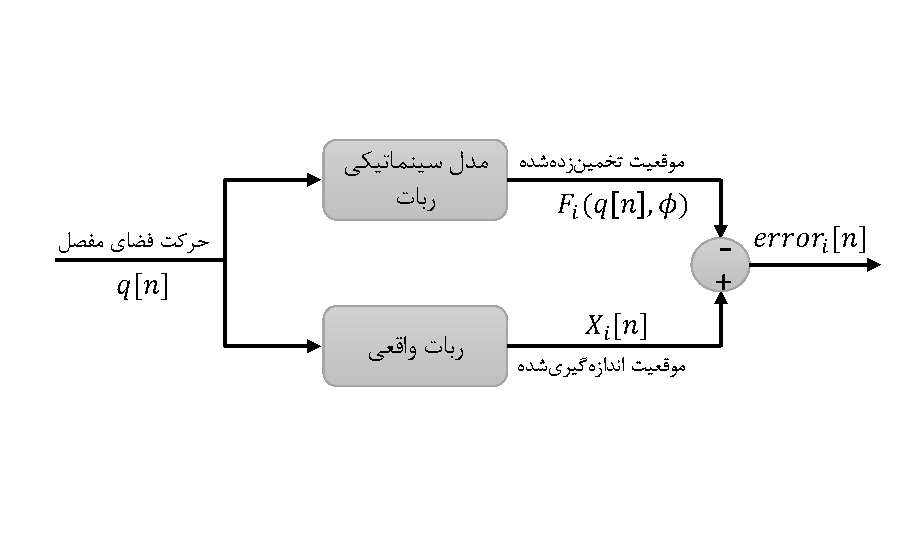
\includegraphics[width=0.8\linewidth, trim={0cm 2.2cm 0cm 2.2cm}, clip]{img/kinematic_model_error}
	\caption{دیاگرام کلی فرمول‌بندی یک مسئله کالیبراسیون}
	\label{fig:kinematicmodelerror}
\end{figure}


با نگاهی به آخرین تحقیقات بر روی مسئله کالیبراسیون ربات ها، ایجاد یک مسئله بهینه سازی غیرخطی و حل آن برای یافتن مقادیر دقیق این پارامتر های سینماتیکی و دینامیکی ربات مرسوم می باشد
\cite{elatta2004overview,ida2019automatic,ida2022identification,ida2021dynamics}.
مطابق این رویکرد های مروسم، برای ایجاد فرمول بندی مناسب مسئله مطرح شده در شکل \ref{fig:kinematicmodelerror} خواهیم داشت:

\begin{equation}\label{eq:optimization_equation_conventional}
	\tilde{\boldsymbol{\phi}} =  \arg\min_{\boldsymbol{\phi}} \sum_{n = 1 }^{N} \text{error}_i[n] = \arg\min_{\boldsymbol{\phi}} \sum_{n = 1}^{N} ||F_i(\boldsymbol{q}[n], \boldsymbol{\phi}) - X_i[n]||^2_{\Sigma}
\end{equation}

در این معادله، $\boldsymbol{\phi}$ بردار پارامتر های سینماتیکی و $\tilde{\boldsymbol{\phi}}$ تخمین آن است. علاوه بر این، $X_i[n]$، 
$iامین$
مقدار اندازه گیری شده توسط حسگر فضای کار ربات، و $\boldsymbol{q}[.]$ مقادیر اندازه گیری های متقابل حسگری در مفاصل می باشد. تابع مدل ربات $F[.]$ بیانگر مدل سینماتیک مستقیم ربات می باشد. تابع هزینه هدف، بر روی مجموعی از $N$ نمونه داده جمع آوری شده در فرآیند کالیبراسیون می باشد. افزون بر این، $\Sigma$ نیز بیانگر ماتریس کوواریانس اندازه گیری می باشد که به عنوان عامل نرمال سازی برای محاسبه هزینه عمل می کند. هر چه مقدار کوواریانس بیشتر باشد، میزان تاثیر گذاری خطای متقابل آن بر روی تابع هزینه کمتر خواهد بود. همچنین برای محاسبه نرم روش های زیادی ارائه شده است که آنچه بیشتر مورد استفاده قرار می گیرد نرم های هابر 
\footnote{\lr{Huber norms}}
می باشد
\cite{chang2015huber}.
معادله بهینه سازی غیر خطی بیان شده در 
\ref{eq:optimization_equation_conventional}
می تواند با روش های بازگشتی الگوریتم های غیر خطی حداقل مربعات
\footnote{\lr{Least-Square}}
همچون  لونبرگ-مارکوارت
\footnote{\lr{Levenberg Marquardt (LM)}}
و یا روش های گاوس-نیوتون
\footnote{\lr{Gauss-Newton(GN)}}
می باشد
\cite{dellart_robot_perception}.

با نگاهی دیگر به دیاگرام مطرح شده در 
\ref{fig:kinematicmodelerror}
و همچنین معادله 
\ref{eq:optimization_equation_conventional}،
مشاهده می‌شود که افزایش دقت اندازه‌گیری و همچنین برآورده کردن تمامی قیود مدل می‌تواند منجر به بهبود نتیجه کالیبراسیون شود. به منظور دستیابی به این هدف، رویکردهایی همچون ترکیب چندین حسگر و یا افزودن قیود جدید که از ساختار هندسی ربات استخراج می‌شود، معرفی می‌شوند. ترکیب این حسگرها باید به گونه‌ای باشد که علاوه بر کاهش خطای نهایی کالیبراسیون، خروج هر کدام از حسگرها منجر به توقف فرآیند کالیبراسیون نشود. همچنین واضح است که افزودن این قیود می‌تواند منجر به حل پیچیده‌تری از مسئله شود. در ادامه، نگاهی به فرمول‌بندی مسئله کالیبراسیون با در نظر گرفتن این ترکیب‌ها خواهیم داشت.

\subsection{ترکیب حسگر ها}
در معادله 
\ref{eq:optimization_equation_conventional}،
زیرنویس 
$i$
بیانگر وجود یک حسگر و خطایی که از مقادیر اندازه گیری حسگر در هر نمونه بوده می باشد. فرمول بندی ساختاری که به صورت همزمان از چندین حسگر در راستای ایجاد تابع هزینه استفاده نماید می تواند به صورت زیر تعریف شود:
\begin{equation}\label{eq:optimization_equation_conventional_multi_sensor}
	\tilde{\boldsymbol{\phi}} =  \arg\min_{\boldsymbol{\phi}} \sum_{n = 1 }^{N} \sum_{n = 1 }^{M} W_i~\text{error}_i[n] 
\end{equation}
در این معادله 
$W_i$
ها یک پارامتر وزن برای ترکیب چندین منبع اطلاعاتی با توجه به میزان کیفیت و اهمیت آنها می باشد.


\subsection{ترکیب شبه اندازه گیری ها}
اندازه گیری های حسگری تنها منبع اطلاعات برای حل مسئله نیستند. ساختار ربات و توحه به هندسه آن برای حل مسئله تعریف شده می تواند مفید واقع شود. برای مثال فاصله های بین برخی از نقاط می تواند با توجه به ساختار ربات می توانند ویژگی هایی نسبی و یا مطلق داشته باشند. این اطلاعات با عنوان داده های شبه اندازه گیری شناخته می شوند. این دسته از اطلاعات که از قبل مشخص هستند، می توانند به صورت قیود به مسئله اضافه شوند. بنابراین مسئله کلی بهینه سازی کالیبراسیون
\ref{eq:optimization_equation_conventional_multi_sensor}
در حضور این قیود به صورت زیر باز نویسی می شود. 
\begin{equation}
	\begin{aligned} \label{eq:optimization_equation_conventional_multi_sensor_measurement}
		&\tilde{\boldsymbol{\phi}} =  \arg\min_{\boldsymbol{\phi}} \sum_{n = 1 }^{N} \sum_{n = 1 }^{M} W_i~\text{error}_i[n] \\
		\quad &g_j(\boldsymbol{\phi}) = 0 \quad where \quad j = 1, \ldots, K
	\end{aligned}
\end{equation}
که در اینجا
$g_j(\boldsymbol{\phi}) = 0$ 
قیود هندسی معلوم بر روی پارامترهای سینماتیکی ربات می باشند.

\section{روش‌های مرسوم مسئله مکان‌یابی}
مکان‌یابی
\footnote{Localization}
 ربات فرآیند تعیین مکان ربات نسبت به محیط اطراف آن می باشد. دانستن مکان دقیق ربات در محیط، پیش‌نیازی اساسی برای اتخاذ تصمیمات صحیح و حرکت های بعدی مؤثر است. بدون اطلاعات مکانی دقیق، ربات نمی‌تواند مسیریابی
\footnote{motion planing}
  و یا ردیابی
\footnote{trakcing}
مناسبی را داشته باشد و ممکن است با موانع برخورد کند یا مسیر بهینه‌ای را طی نکند
\cite{ahmad2013cooperative}.
 علاوه بر این، سیستم‌های کنترلی ربات‌ها نیازمند اطلاعات دقیق و لحظه‌ای از مکان و جهت‌گیری ربات هستند تا بتوانند فرمان‌های مناسب را صادر کنند. بدون داده‌های دقیق مکانی، کنترلرها نمی‌توانند حرکات دقیقی را تولید کنند که منجر به عملکرد نامناسب و ناپایداری ربات می‌شود
\cite{guibas1997robot}.
فرآیند کالیبراسیون ربات که در بخش 
\ref{seq:conventional_calibration}
مورد بررسی قرار گرفت نیز یازمند داشتن اطلاعات دقیق از مکان ربات است. با داشتن داده‌های مکانی دقیق، می‌توان خطاهای سیستماتیک را شناسایی و تصحیح کرد و به این ترتیب دقت و کارایی ربات را بهبود بخشید. این امر به ویژه در ربات‌هایی که نیاز به انجام وظایف حساس و دقیق دارند، حیاتی است. 

مکان‌یابی دقیق ربات باعث کاهش عدم قطعیت در تصمیم‌گیری‌ها و عملیات ربات می‌شود. این امر نه تنها به افزایش اعتمادپذیری ربات در انجام وظایف محوله منجر می‌شود، بلکه احتمال بروز خطاها و حوادث ناشی از اشتباهات مکانی را نیز کاهش می‌دهد. همچنین در سیستم‌هایی که شامل چندین ربات هستند، اطلاعات دقیق مکانی هر ربات برای هماهنگی و همکاری بین ربات‌ها ضروری است. این اطلاعات به ربات‌ها کمک می‌کند تا از مکان یکدیگر آگاه باشند و بتوانند به صورت هماهنگ وظایف مشترک را انجام دهند. در این راستا توسعه و بهبود تکنیک‌های مکان‌یابی به منظور افزایش دقت و کارایی ربات‌ها، از اهمیت ویژه‌ای برخوردار است
\cite{aragues2011multi}.


روش های ارائه شده برای مکان‌یابی ربات را می توان به سه دسته اصلی مسافت پیمایی
\footnote{odometry}،
مکان‌یابی جهانی
\footnote{global localization}
و مکان یابی و نقشه یابی به صورت همزمان
\footnote{SLAM}
تقسیم کرد. این روش ها با توجه به نوع حسگرهای تعبیه شده بر روی ربات می تواند مورد استفاده قرار گیرد. ترکیب داده ها برای همانند آنچه در بخش
\ref{seq:conventional_calibration}
مورد توجه قرار گرفت، در مکان‌یابی و تخمین حالت ربات نیز می تواند نقش موثری را ایفا کند. حسگر های استفاده شده از نظر جنس داده ها و فرکانس داده برداری نیز می تواند متفاوت باشد که در ترکیب داده ها خصوصا زمانی که اجرای الگوریتم به صورت زمان واقعی می باشد، چالش برانگیز خواهد بود. طیف وسیعی از روش های مرسوم ارائه شده برای ترکیب داده ها در راستای تخمین حالت، رویکردهای بر مبنای فیلتر هستند. این روش ها که به رویکرهای آماری 
\footnote{stochastic}
نیز شناخته می شوند، در دو دهه اخیر فعالیت های زیادی را به خود اختصاص داده اند. پایه این روش ها بر قانون بیز
\footnote{Bayes law}
بنا نهاده شده است. مقاله
\cite{panigrahi2022localization} 
دسته بندی جامعی از روش های فیلتر مبنا برای تخمین مکان ارائه کرده است. از میان روش های بیان شده، کالمن فیلتر و فیلترهای ذرات
\footnote{particle filters}
به عنوان فراگیرترین رویکرد مورد استفاده قرار گرفته شده است. این فیلترها با استفاده از فرض مارکووی برای حالت ها و به کار گیری اطلاعات پیشین، تخمینی از حالت جدید ارائه می کنند. 

\section{رویکرد گراف مبنا برای حل مسئله کالیبراسیون و مکان‌یابی به صورت همزمان}
روش‌های مرسوم کالیبراسیون و مکان‌یابی ربات‌ها که تا به اینجا معرفی شده‌اند، فرمول‌بندی‌های مشخصی برای حل این دو مسئله ارائه داده‌اند. همانطور که در فصل قبل مشاهده شد، سادگی و سرعت بالای این روش‌ها باعث پیاده‌سازی گسترده آن‌ها گردیده است. با این حال، این روش‌ها دارای معایبی نیز هستند. 
اول اینکه برای هر مسئله کالیبراسیون و ربات، فرمول‌بندی مسئله باید از ابتدا توسعه داده شود. دوم اینکه  این روش‌ها از تنک بودن ذاتی مسئله‌ها برای سرعت بخشیدن به محاسبات استفاده نمی‌کنند.  بزرگ شدن و پیچیده شدن فرمول‌بندی این مسائل باعث می‌شود که از حل آن‌ها به صورت زمان واقعی فاصله گرفته شود.  همچنین، این روش‌ها برای حل مسائل غیرخطی نیاز به خطی‌سازی دارند که نه تنها به پیچیدگی‌های محاسباتی می‌افزاید، بلکه باعث کاهش دقت نیز می‌شود. 
سومین موضوع،  روش‌های مرسوم فیلتر مبنا از داده‌های جاری و لحظه‌ای استفاده می‌کنند که باعث می‌شود علاوه بر مشکلات در مدیریت داده‌هایی که با تأخیر به سیستم می‌رسند، نتوانند داده‌های تاریخی را به صورت کامل در یک مسئله بهینه‌سازی دسته‌ای وارد کنند. این مشکل در مسائل مکان‌یابی باعث ایجاد مشکلات جدی همچون لغزش
\footnote{drift}
و کاهش دقت تا حد قابل توجهی می‌شود. چهارمین عیب این روش‌ها، عدم انعطاف‌پذیری آن‌ها برای بسط دادن مسئله با افزودن قیود به سیستم یا داده‌های حسگری به آن است. با توجه به این معایب، روش‌های مرسوم ممکن است در برخی کاربردهای پیشرفته رباتیک کارایی لازم را نداشته باشند. 

در این فصل، رویکردی گراف مبنا برای حل مسئله کالیبراسیون و مکان‌یابی ربات بیان می‌گردد که با فرمول‌بندی یکپارچه، هر دو مسئله را به صورت همزمان در یک مسئله بهینه‌سازی حل می‌کند. ویژگی‌های ذاتی این رویکرد در حل این مسئله واحد به تمامی معایب مطرح شده در روش‌های مرسوم پاسخ می‌دهد و باعث ایجاد حلی کامل و قابل بسط می‌شود. این رویکرد گراف مبنا به دلیل استفاده از ساختارهای گرافی، قادر به مدیریت بهینه‌تر داده‌های مختلف است. با ادغام تمامی داده‌های تاریخی و جاری در یک مسئله بهینه‌سازی دسته‌ای، این روش از داده‌های ورودی به صورت کامل استفاده کرده و به مشکلات مدیریت داده‌های تأخیر دار و لحظه‌ای غلبه می‌کند. همچنین، به دلیل عدم نیاز به خطی‌سازی مکرر، دقت محاسبات افزایش یافته و پیچیدگی‌های محاسباتی کاهش می‌یابد. علاوه بر این، انعطاف‌پذیری بالای این رویکرد امکان افزودن قیود و داده‌های حسگری جدید را فراهم می‌کند، بدون آن که نیاز به بازتعریف کلی فرمول‌بندی باشد. این ویژگی‌ها، در کنار توانایی بهره‌گیری از تنک بودن ذاتی مسئله‌ها برای بهینه‌سازی محاسبات، این رویکرد گراف مبنا را به یک ابزار قدرتمند برای کالیبراسیون و مکان‌یابی ربات‌ها تبدیل می‌کند.

الگوریتم گراف مبنای استفاده شده برای این فرمول‌بندی در این پایان‌نامه، الگوریتم گراف عامل
\footnote{factor graph}
می‌باشد. در ادامه، ابتدا نگاهی بر ریاضیات مرتبط با الگوریتم گراف عامل خواهیم داشت و سپس گراف عامل یکپارچه‌ای را برای حل مسئله مطرح شده معرفی خواهیم کرد. گراف عاملی که در ادامه پیشنهاد خواهد شد، حلی سیستماتیک برای کنار هم قرار دادن بلوک‌های ساختاری (عامل‌ها) در راستای تعریف یک مسئله کالیبراسیون در کنار مسئله مکان‌یابی به صورت یکپارچه است، که قابلیت گسترش به حسگرهای بیشتر و قیود اضافی را نیز دارا می‌باشد. علاوه بر این، از آنجایی که پیاده‌سازی‌های منابع باز و بهینه‌سازی شده برای این روش وجود دارد، مسئله کالیبراسیون و مکان‌یابی همزمان مطرح شده می‌تواند بر روی سیستم‌های نهفته بر روی ربات نیز پیاده‌سازی گردد. در این پایان‌نامه برای پیاده‌سازی گراف عامل پیشنهاد داده شده، از کتابخانه GTSAM استفاده شده است. 

\subsection{بیان الگوریتم گراف عامل}
مسئله غیرخطی تعریف شده در 
\ref{eq:optimization_equation_conventional_multi_sensor_measurement}
می‌تواند به‌صورت یک مدل گرافی که متشکل از گره‌هایی است که بیانگر متغیرهای تصمیم‌گیری هستند و یال‌هایی که ارتباط بین قیود و این متغیرها را نشان می‌دهند، بیان شود. در جامعه رباتیک، گراف عامل نمونه‌ای از این بیان است. این گراف‌ها یک چارچوب قوی و قابل انطباق برای بیان مسائل متنوع از تخمین حالت
\footnote{state estimation}
 تا برنامه‌ریزی حرکت
\footnote{motion planning}
 ، ارائه می‌دهند.  این الگوریتم برای حل مسائل بهینه‌سازی که شامل متغیرهای مختلف و قیود پیچیده است، مناسب می‌باشد. یکی از روش‌های بیان این مدل، استفاده از نمودارهای دو بخشی
$\boldsymbol{F} = (\mathcal{U}, \mathcal{V}, \mathcal{E})$
است که  عامل‌ها 
$(\mathcal{U})$
با استفاده از یال‌ها
$(\mathcal{E})$
روابط و قیودی را بین گره‌ها 
$(\mathcal{V})$
 ایجاد می‌کنند. بدین ترتیب بخش اول، یعنی گره‌ها، نمایانگر متغیرهای ناشناخته یا پارامترهای مدل هستند که آنها را با
$\boldsymbol{\phi_i}$
نشان می‌دهیم. به عنوان مثال، در مسئله کالیبراسیون و مکان‌یابی، گره‌ها می‌توانند نمایانگر مکان‌های مختلف ربات یا پارامترهای کالیبراسیون باشند. همچنین بخش دوم، یعنی عامل‌ها، نشان‌دهنده قیود یا روابط بین متغیرها می‌باشد که آنها را با
$\psi_i$
نشان می‌دهیم. این قیود می‌توانند شامل معادلات غیرخطی یا روابط پیچیده‌ای باشند که باید در فرآیند بهینه‌سازی در نظر گرفته شوند. بدین ترتیب یک گراف عامل 
$\boldsymbol{F}$
بیان کننده نحوه ایجاد یک تابع انرژی کلی
$\boldsymbol{\psi}$
از تک تک اجزای سیستم می باشد:
\begin{equation} 
	\boldsymbol{\psi}(\boldsymbol{\phi}) = \prod_{i} \boldsymbol{\psi}_i(\boldsymbol{\phi}_i) 
\end{equation}
کمینه‌سازی لگاریتم تابع 
$\boldsymbol{\psi}(\boldsymbol{\phi})$
منجر به ایجاد یک مسئله غیرخطی معادل می‌شود که مسئله بهینه‌سازی مورد نظر را مشخص می‌کند.


\subsection{گراف عامل پیشنهادی برای کالیبراسیون و مکان یابی به صورت همزمان}
  
همانطور که بیان شد، استفاده از گراف‌های عامل در مکان‌یابی ربات‌ها مزایای متعددی دارد. یکی از مزایای اصلی این است که گراف عامل می‌تواند به طور مؤثری اطلاعات نامطمئن را مدیریت کرده و تخمین‌های دقیق‌تری ارائه دهد. همچنین، این روش به دلیل ساختار گرافی خود، قابلیت انعطاف‌پذیری و مقیاس‌پذیری بالایی دارد، به طوری که می‌توان به راحتی اندازه‌گیری‌های جدید را به گراف اضافه کرده و تخمین‌ها را به‌روزرسانی کرد. در مسئله‌ی مکان‌یابی ربات‌ها، هدف اصلی تخمین دقیق مکان و جهت ربات در محیط است. برای این منظور، از اطلاعات مختلفی مانند داده‌های حسگرها، اندازه‌گیری‌های فاصله و داده‌های اینرسی استفاده می‌شود. گراف عامل این اطلاعات را به شکلی یکپارچه و هماهنگ ترکیب می‌کند.

برای مدل‌سازی مسئله مکان‌یابی با گراف عامل، ابتدا باید متغیرهای حالت ربات و محدودیت‌های مرتبط با آنها تعریف شوند. متغیرهای حالت می‌توانند شامل مکان و جهت پنجه ربات در نقاط مختلف زمانی نسبت به یک چارچوب پایه مشخص باشند. برای تعریف این متغیرهای حالت در زمان $i$ با کمک ماتریس انتقال پنجه ربات در فضای
$SE(3)$
به صورت زیر خواهد بود:
\begin{equation} \label{eq:transformation matrix}
	\boldsymbol{X}_i = \begin{bmatrix}
							\mathbf{R}_i & \mathbf{t}_i \\
								0 & 1
				     	\end{bmatrix}
\end{equation}
که 
$\boldsymbol{X}_i^{4\times4}$
 بیانگر ماتریس انتقال شامل ماتریس چرخش 
$\mathbf{R}_i^{3\times3}$
 و بردار انتقال 
 $ \mathbf{t}_i^{3\times1}$ 
 نسبت به چارچوب پایه می‌باشد. علاوه بر تعیین چارچوب پایه در حل مسئله مکان‌یابی، محدودیت‌ها نیز می‌توانند
شامل اندازه‌گیری‌های حسگرهای متفاوت باشد. 
 ما در این فرمول بندی
 حسگر اندازه‌گیری‌های اینرسی
\footnote{IMU} 
 و یک حسگر فاصله‌پیمایی چشمی
\footnote{Visual Odometry}
را به عنوان داده‌های اندازه‌گیری سیستم با فرکانس‌های متفاوت در نظر می‌گیریم. 

شکل 
\ref{fig:localization}
نشان‌دهنده گراف عاملی است که برای حل مسئله مکان‌یابی با فرضیات در نظر گرفته شده می‌توان ارائه کرد. دایره‌ها نشان‌دهنده متغیرهای مسئله هستند که در اینجا مکان ربات می‌باشند و آن‌ها را با ماتریس
$\boldsymbol{X}_i$ 
در زمان $i$ نمایش می‌دهد. مربع‌های رنگی نشان‌دهنده محدودیت‌ها و داده‌های حسگری هستند که با گذر زمان به سیستم وارد می‌شوند و زنجیره مکان ربات را نیز امتداد می‌دهند. چارچوب پایه تعیین شده که می‌تواند نقطه شروع یا نقطه استراحت ربات باشد، توسط یک عامل واحد
\footnote{unary factor}
(در اینجا مربع قرمز رنگ)، مکان‌یابی ربات را مقید می‌کند. همچنین داده‌های حسگری با توجه به فرکانس داده‌برداری آن‌ها می‌توانند به صورت عامل‌های دودویی که بین دو یا چند متغیر قیدی را ایجاد می‌کنند، وارد مسئله شوند. در این گراف، عامل‌های مشخص شده با رنگ سبز نشان‌دهنده اندازه‌گیری‌های حسگر اینرسی و همچنین اطلاعات حسگر فاصله‌پیمایی چشمی با عامل‌هایی به رنگ آبی وارد مسئله می‌شوند. با توجه به نرخ اضافه شدن این اطلاعات به سیستم، می‌توان دریافت که فرکانس داده‌برداری از حسگر اینرسی دو برابر حسگر فاصله‌پیمایی است. 
\begin{figure}
	\centering
	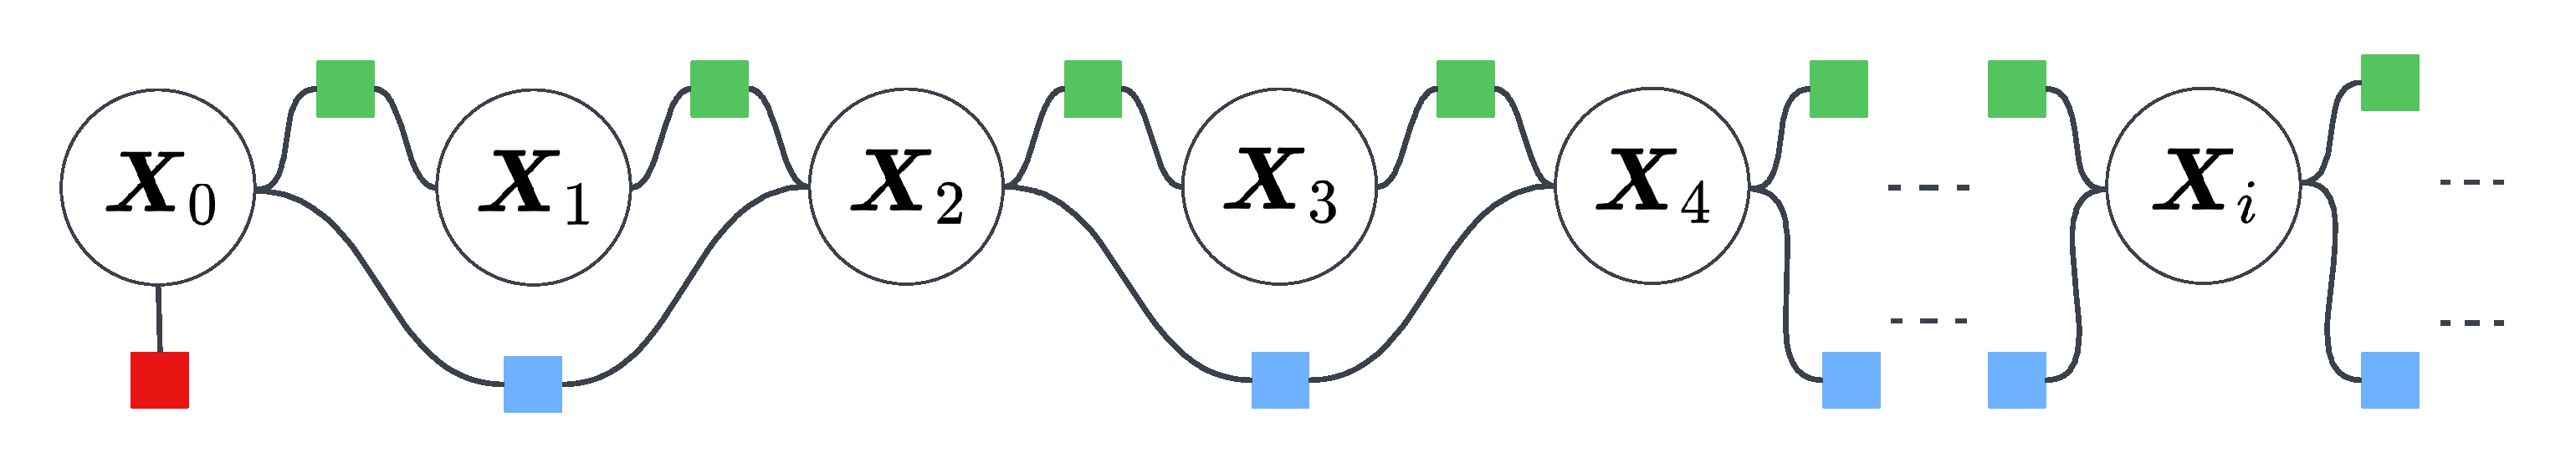
\includegraphics[width=0.7\linewidth]{img/Localization}
	\caption{گراف عامل پیشنهادی برای یک حل یک مسئله مکان‌یابی}
	\label{fig:localization}
\end{figure}

در این گراف، آنچه باعث حل یکپارچه و استفاده بهینه از تمامی اطلاعات مسئله می‌شود، زنجیره‌ای است که میان متغیرهای مسئله ایجاد شده است. با دریافت هر داده جدید از حسگر، یک متغیر مکان جدید برای ربات ایجاد می‌شود که حل مسئله بهینه‌سازی برای پیدا کردن این متغیر منجر به به‌روز رسانی تمامی گره‌ها به‌صورت یکجا می‌شود و این باعث ایجاد یک راه‌حل ارزشمند برای یک مسئله تنک می‌گردد. در این بخش، هدف تعریف پایه‌ای یک مسئله مکان‌یابی برای ربات است. گراف‌های متنوع و فرمول‌بندی‌شده برای اهداف خاص‌تر در
\cite{yang2022indoor}, 
\cite{song2021tightly}
و 
\cite{leitinger2017factor}
قابل مطالعه هستند. 

افزودن حسگرهای جدید با ایجاد گره‌های عامل با مدل نویزهای مناسب در فواصل زمانی منظم، می‌تواند نتیجه مکان‌یابی را بهبود بخشد. این ترکیب حسگرها می‌تواند در فواصل زمانی‌ای که حسگرها به‌دلیل شرایط محیطی از سیستم خارج می‌شوند، از توقف مکان‌یابی جلوگیری کند. به‌عنوان مثال، الگوریتم‌هایی که از داده‌های دوربین استفاده می‌کنند، زمانی که ویژگی‌های محیط برای پردازش تصاویر نامناسب است یا ربات وارد محدوده‌ای تاریک می‌شود، قادر به ارائه نتایج مناسبی نیستند. به عنوان نمونه‌ای دیگر، زمانی که سیستم مکان‌یابی جهانی
\footnote{GPS}
مورد استفاده قرار می‌گیرد، مکان‌هایی همچون تونل‌ها می‌توانند این سیستم جمع‌آوری داده را با مشکل مواجه کنند. بدین ترتیب، با خروج برخی از حسگرها مکان‌یابی با استفاده از داده‌های دیگر انجام می‌شود و با ورود مجدد حسگرها، نتایج رو به بهبود خواهند رفت. استفاده از این رویکرد محدود به نوع ربات و یا حسگرهای آن نبوده است.  
از ربات‌های خودران
\cite{wilbers2019localization}
تا ربات‌های پرنده
\cite{dai2022uav}
و یا ربات‌های جراح مورد استفاده در اتاق های عمل می توانند از این روش استفاده کنند. 


استفاده از گراف در مسئله مکان‌یابی برای ربات‌های چندعاملی می‌تواند کلیدی برای بهبود نتایج و فرمول‌بندی ساده‌تر باشد. سامانه آموزش جراحی چشم 
ARASH:ASiST 
در تیم آزمایشگاهی ارس توسعه یافته است
\cite{hassani2021kinematic}. این سامانه از دو دستگاه ربات مجزا برای تسهیل فرآیند آموزش جراحی تشکیل شده است. در این سامانه، ربات دوم باید حرکات ربات اول را دنبال کند تا آموزش جراحی با استفاده از این سامانه انجام پذیرد. پیدا کردن چارچوب این ربات‌ها در یک دستگاه مختصات می‌تواند یکی از ابزارهایی باشد که در پیاده‌سازی الگوریتم‌های متنوع کنترلی در فرآیند یادگیری مهارت مورد استفاده قرار گیرد. یکی از روش‌های پیشنهادی برای این هدف می‌تواند استفاده از گراف شکل 
\ref{fig:arashasistlocalization}
باشد. در این گراف، مکان‌یابی برای هر کدام از این ربات‌ها با به‌روز رسانی
$\boldsymbol{X}_{i}$
و
$\boldsymbol{X}_{i}^{'}$
برای هر یک از ربات‌ها به صورت مجزا، انجام می‌شود. هم‌چارچوب‌سازی این دو ربات می‌تواند توسط قیود عاملی که در اینجا با رنگ نارنجی نشان داده شده است، انجام شود. دیگر عامل‌ها با رنگ‌های مشخص شده همانند تعاریف بیان شده در شکل 
\ref{fig:localization}
می‌باشند. 

\begin{figure}
	\centering
	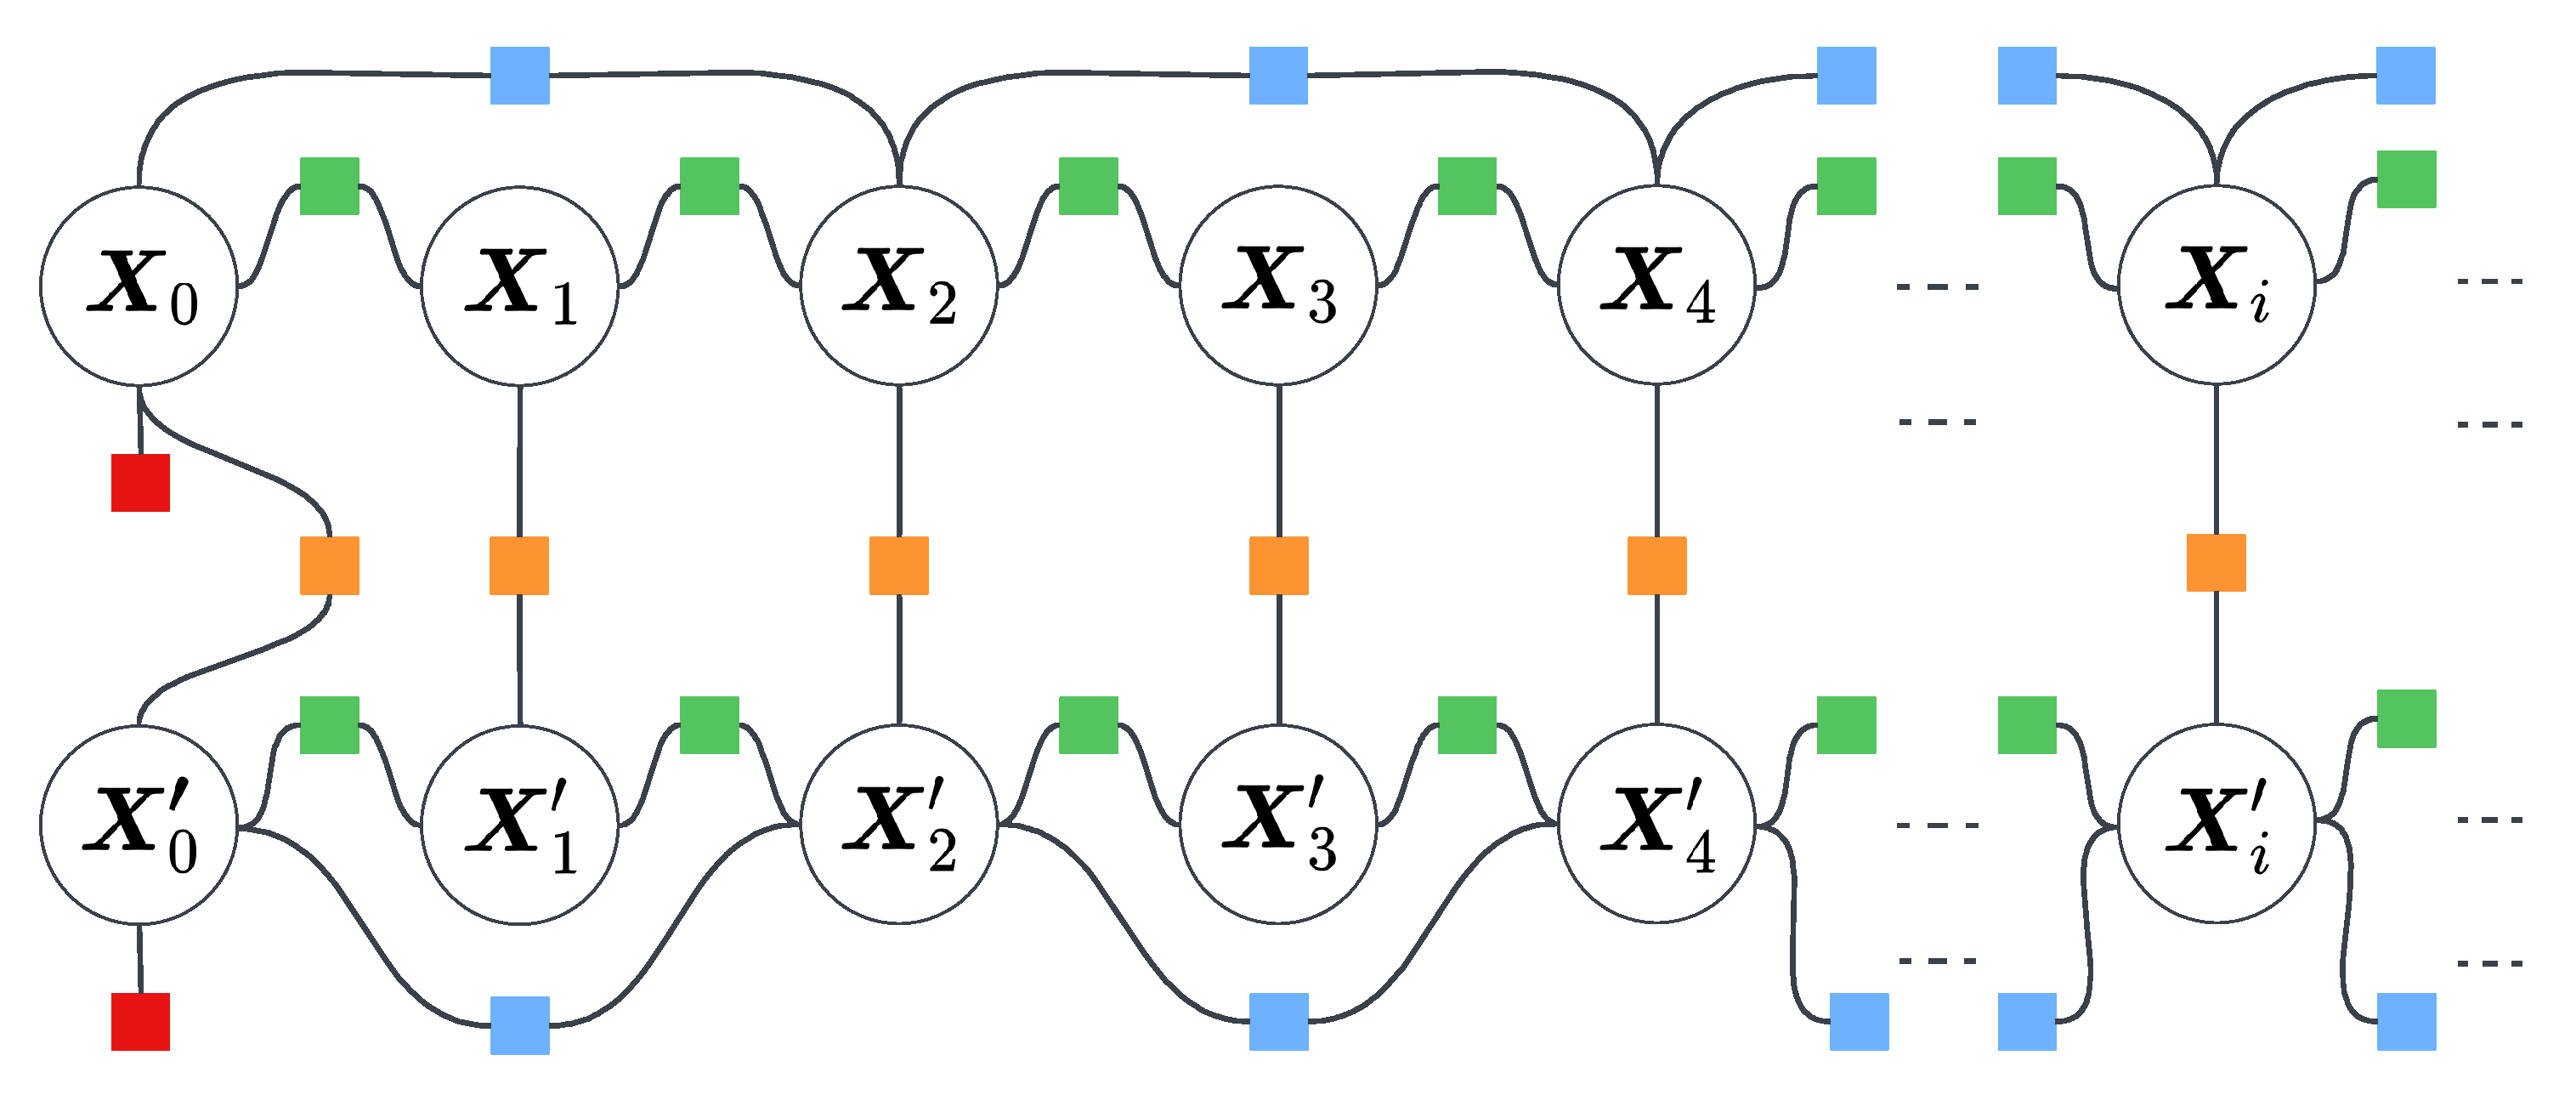
\includegraphics[width=0.7\linewidth]{img/Arash_Asist_localization}
	\caption{گراف عامل پیشنهادی برای یک حل یک مسئله مکان‌یابی ربات‌های چند عاملی}
	\label{fig:arashasistlocalization}
\end{figure}


آنچه تا بدین جای حل مسئله مشاهده شده است، توانایی بالای الگوریتم گراف عامل در ایجاد مسئله‌ای انعطاف‌پذیر بوده است. مقیدسازی این مسئله می‌تواند از قیود فضای کار ربات فراتر رفته و مسئله را در فضای مفصلی و ساختار سینماتیک ربات نیز مقید کند. وجود پارامترهای سینماتیکی در فرمول‌بندی می‌تواند با در نظر گرفتن آنها به‌عنوان متغیرهایی که همواره در ربات ثابت هستند یا متغیرهایی که با گذر زمان تغییر می‌کنند، به‌عنوان پارامترهای کالیبراسیون، مقادیر بهینه آنها را به‌دست آورد. به عبارتی، در حالی که مسئله مکان‌یابی در حال انجام است، مسئله کالیبراسیون نیز حل شود. همچنین اضافه شدن این قیود سینماتیکی می‌تواند مکان‌یابی ربات را بهبود بخشد.

مطابق فرمول‌بندی‌های مرسوم ارائه شده، معادلات سینماتیک نگاشت‌های غیرخطی بین فضای مفصل و فضای کار ربات ایجاد می‌شوند. بدین ترتیب:
\begin{equation} \label{eq:IK_FK_genral_equations}
	\boldsymbol{X} = FK(\boldsymbol{q}, \boldsymbol{\phi}), ~~ \boldsymbol{q} = IK(\boldsymbol{X}, \boldsymbol{\phi})
\end{equation}
که
$\boldsymbol{X}$
مکان ربات در فضای کار و
$\boldsymbol{q}$
بردار مقدار زاویه‌ای/طولی مفصل‌های ربات هستند. در این معادله
$\boldsymbol{\phi}$
بردار پارامترهای سینماتیکی ربات است که به هندسه ساختاری ربات مربوط می‌شود.

در ادامه، با فرض آنکه ربات مسیری تصادفی را در فضای کاری خود طی می‌کند و همچنین داده‌های سنسوری در هر دو فضای معرفی شده در حال جمع‌آوری هستند، قصد داریم گراف
\ref{fig:localization}
را به گونه‌ای بسط دهیم که کالیبراسیون سینماتیکی ربات در کنار مکان‌یابی در یک گراف یکپارچه حل شود. برای این کار از قیود سینماتیکی
\ref{eq:IK_FK_genral_equations}
استفاده کرده و آنها را به‌صورت عامل به مسئله می‌افزاییم. ابتدا فرض کالیبراسیون را بر ثابت بودن پارامترهای سینماتیکی و عدم تغییر آنها در طول زمان می‌گذاریم. شکل
\ref{fig:kinematiclocalizationbasic}
بیانگر یک گراف برای حل این مسئله با این فرض بیان شده می‌باشد. در این گراف، قسمت مکان‌یابی همانند آنچه پیشتر بیان شد می‌باشد. همچنین عامل‌های مشخص شده با مربع‌های سیاه رنگ بیانگر روابط سینماتیکی ربات هستند که تابعی از مقادیر متغیرهای مفصل، مکان ربات در فضای کار و بردار پارامترهای سینماتیکی ربات
 $\boldsymbol{\phi}$
 می‌باشند. همچنین عامل‌های خاکستری رنگ بیانگر مقادیر اندازه‌گیری شده در فضای مفصل ربات از حسگرهای آن می‌باشند. 
\begin{figure}
	\centering
	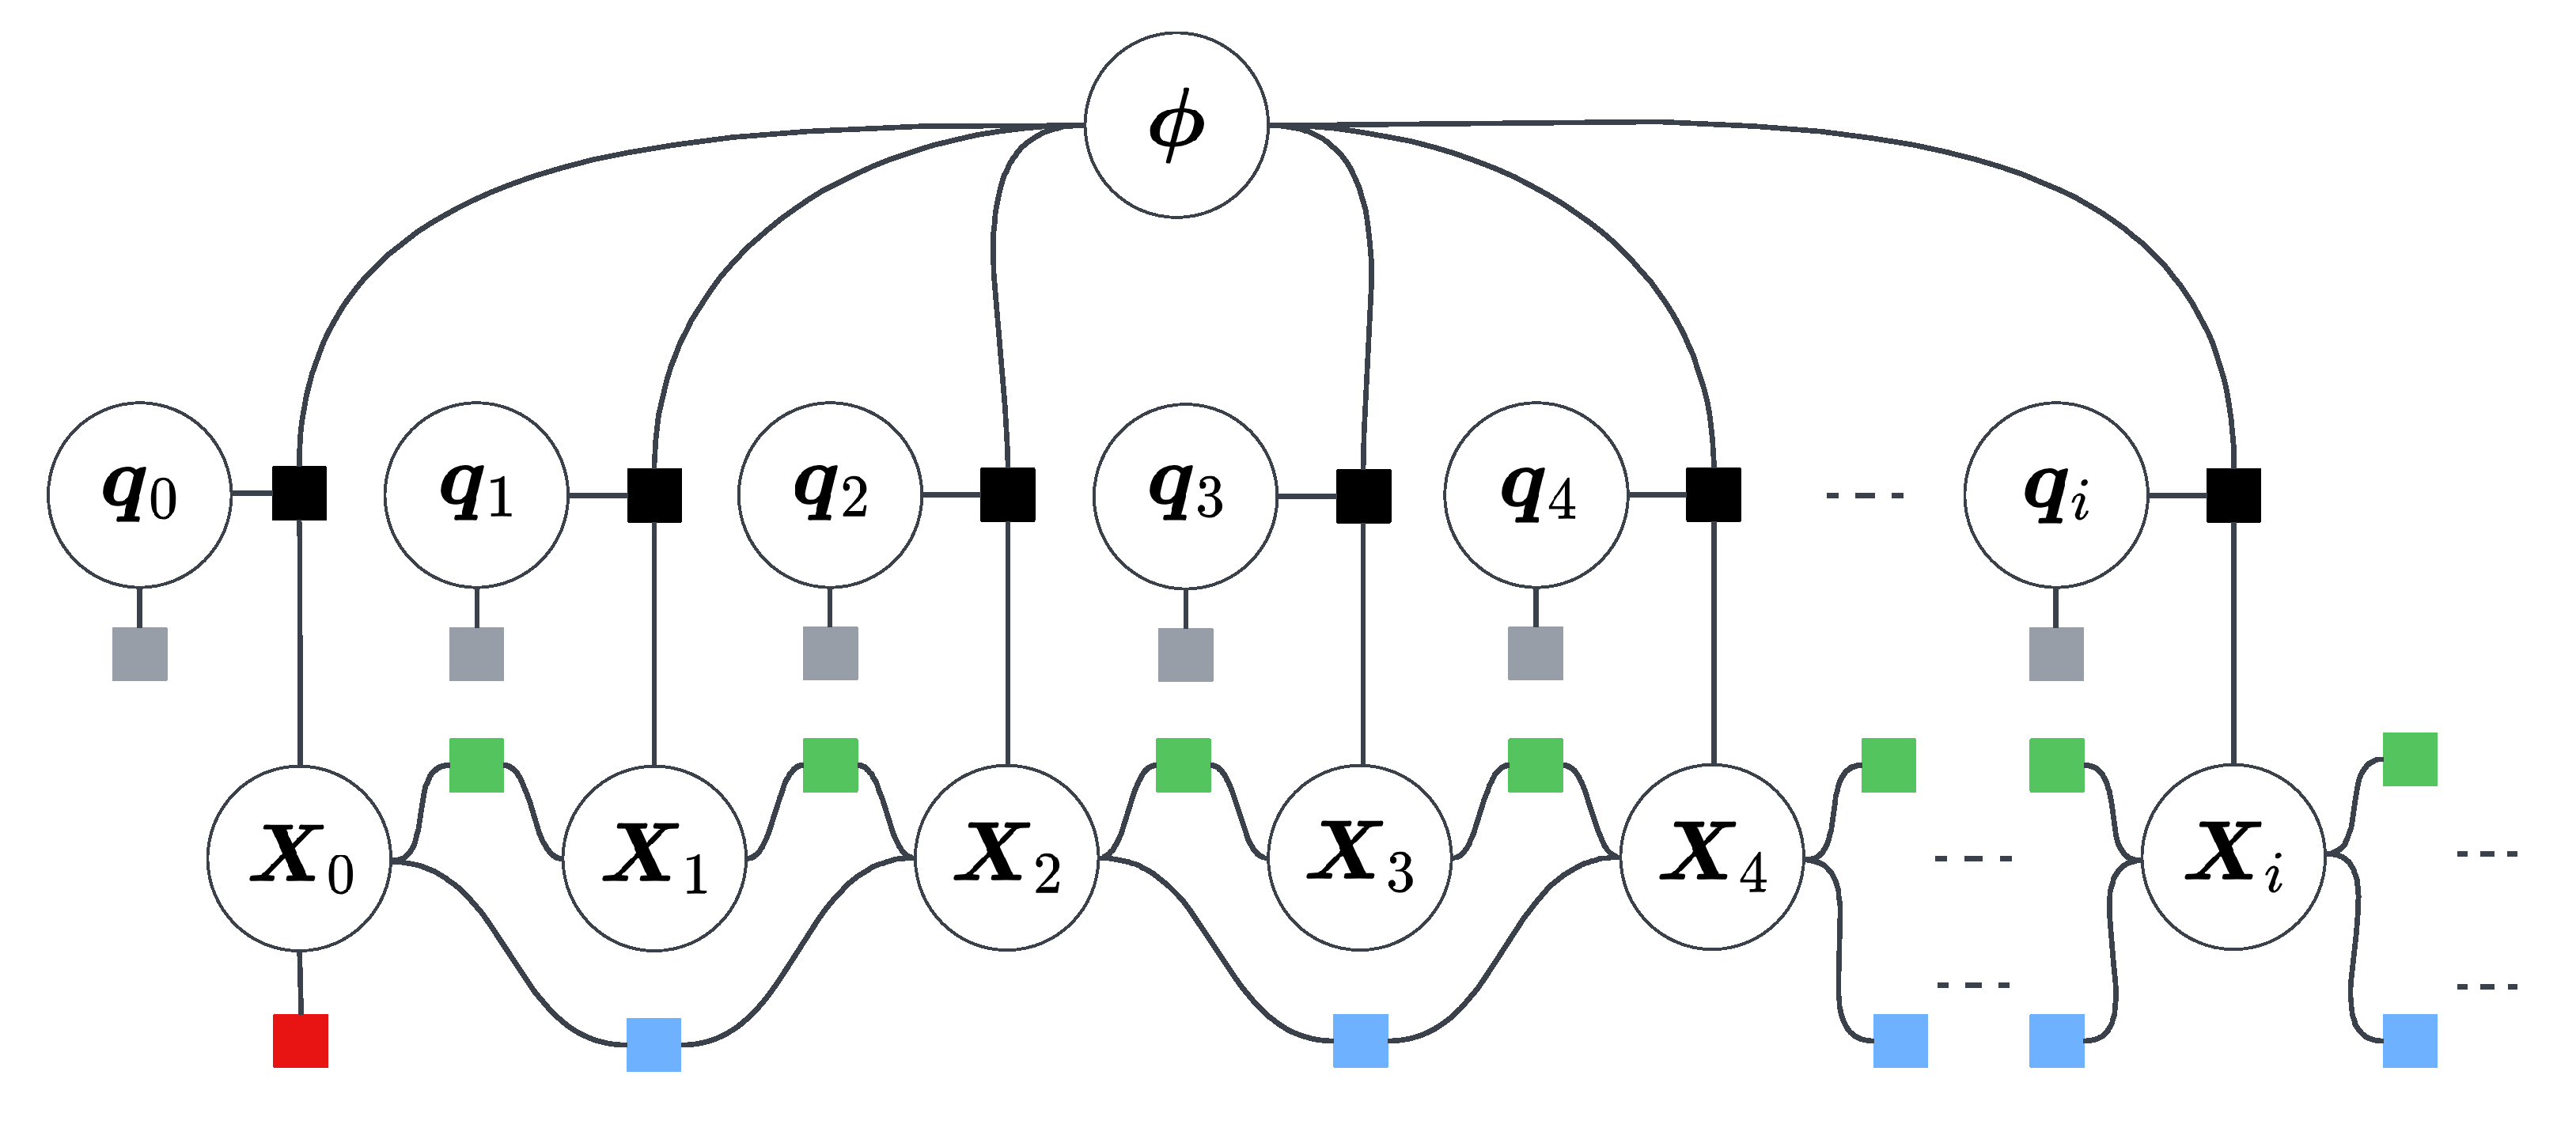
\includegraphics[width=0.7\linewidth]{img/Kinematic_localization_basic}
	\caption{گراف عامل پیشنهادی برای مسئله مکان‌یابی و کالیبراسیون همزمان با پارامتر‌های نامتغیر با زمان}
	\label{fig:kinematiclocalizationbasic}
\end{figure}

فرمول‌بندی سینماتیک بیان‌شده در 
\ref{eq:IK_FK_genral_equations}
می‌تواند طیف وسیعی از ربات‌ها را در بر داشته باشد. به عنوان نمونه، برای روشن‌سازی بهتر مسئله، نمونه موردی ربات
ARASH:ASiST
را باری دیگر در نظر می‌گیریم. شکل
\ref{fig:arashasiststructure}
شمایی از هندسه با ساختاری متوازی‌الاظلاع از این ربات را نشان می‌دهد. پارامترهای سینماتیک این ربات با بردار
$\boldsymbol{\phi} = \{ \alpha, \theta , l_{1234} \} $
مطابق اندازه‌های بیان‌شده بر روی این شکل تعریف می‌شود. همچنین با توجه به مقادیری که بردار مفاصل ربات 
$ \boldsymbol{q}=\{ \phi, \psi, d \} $
دارند، مکان پنجه ربات
$\boldsymbol{X}$
در نقطه دوران از راه دور مشخص شده‌است. با استفاده از این بیان، ساختار سینماتیکی این ربات می تواند به فرمول‌بندی سینماتیک  مستقیم زیر مطابق آنچه در
\cite{hassani2021kinematic}
استخراج شده است، منجر شود:
\begin{equation} \label{eq:arash_asist_fk}
		\begin{aligned}
			\left( \begin{array}{c}
				x \\
				y \\
				z 
			\end{array} \right)
			&=
			\left( \begin{array}{c}
				c_{\theta}(l_{1234} + dc_{\alpha + \psi}) - ds_{\theta}c_{\phi}s_{\alpha + \psi} \\
				s_{\theta}(l_{1234} + dc_{\alpha + \psi}) + d c_{\theta}c_{\phi}s_{\alpha + \psi} \\
				ds_{\phi} s_{\alpha + \psi}
			\end{array} \right)
		\end{aligned}
\end{equation}
که $s$ و $c$ به ترتیب بیانگر توابع 
$\sin(.)$
و
$\cos(.)$
هستند. تفسیر مکان‌یابی و کالیبراسیون سینماتیکی بیان شده در گراف
\ref{fig:kinematiclocalizationbasic}،
استفاده از معادله
\ref{eq:arash_asist_fk}
در عامل‌های بیان شده به عنوان قیود سینماتیکی ربات (عامل‌های سیاه) است. 

\begin{figure}
	\centering
	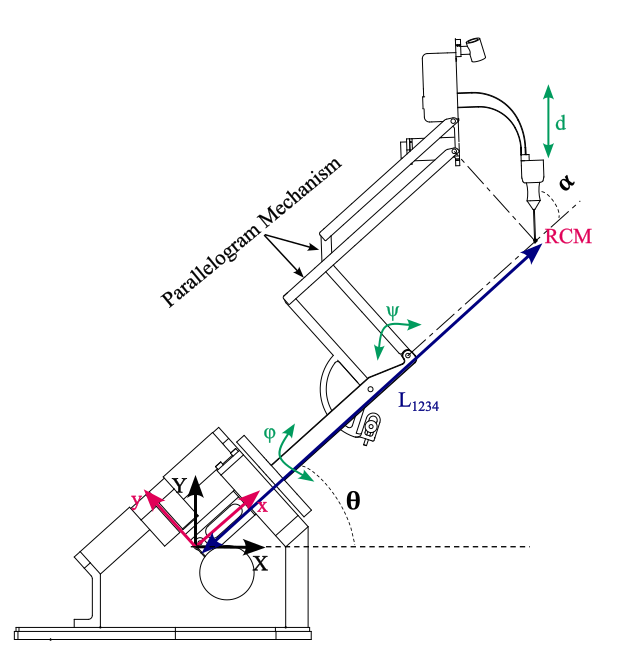
\includegraphics[width=0.5\linewidth]{img/ARASH_ASIST_Structure}
	\caption{نمایی از ساختار ربات ARASH:ASiST}
	\label{fig:arashasiststructure}
\end{figure}

شکل 
\ref{fig:kinematiclocalizationbasicnonstationatyparam}
نشان دهنده گراف قابل استفاده دیگری می باشند که عاری از فرض ثابت بودن پارامترهای کالیبراسیون سینماتیکی بوده و این پارامترها با گذر زمان تغییر می کند و در مسائل زمان واقعی چالش برانگیز هستند. عامل های زرد ایجاد شده در بین پارامترهای کالیبراسیون در زمان های متوالی قیودی هستند که از نوسانات و تغیرات ناگهانی و زیاد این پارامتر های جلوگیری کنند. وجود این قید از آنجایی است که در دنیای واقع انتظار بر تغیر آهسته و منطقی این پارامترهای هندسی می باشد. 
با این بیان صورت گرفته، افزودن قیود متفاوت به مسئله بدون نیاز به تغییر فرمول‌بندی دیگر بخش‌ها قابل انجام خواهد بود. در نهایت، این گراف‌های عامل می‌توانند با استفاده از حل‌کننده‌های افزایشی که کتابخانه GTSAM در اختیار ما قرار می‌دهد، به‌صورت زمان واقعی حل شوند. 

\begin{figure}[b]
	\centering
	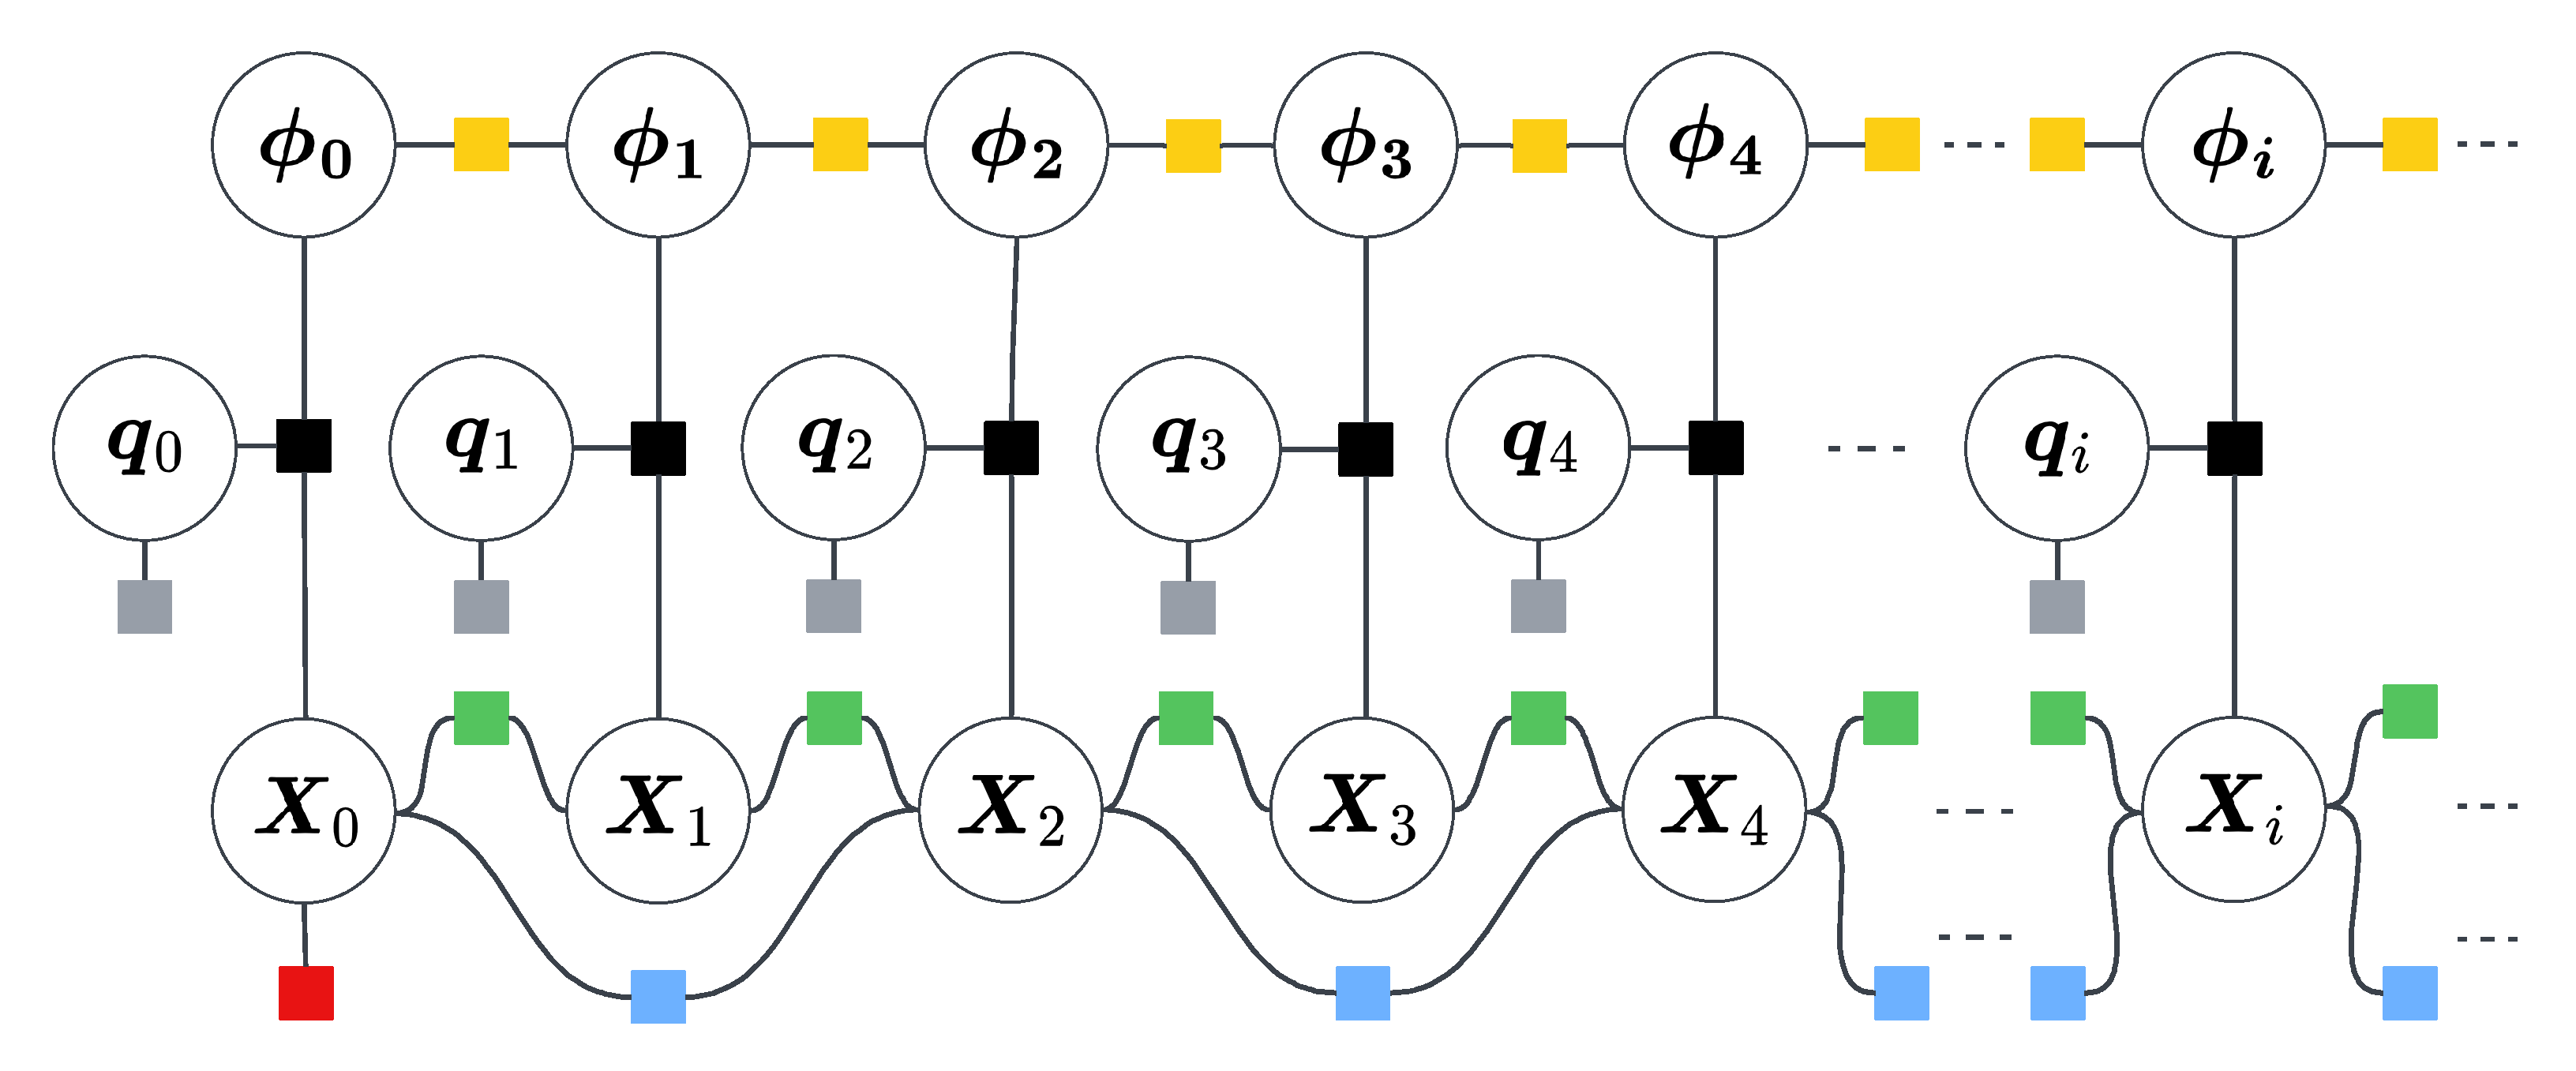
\includegraphics[width=0.7\linewidth]{img/Kinematic_localization_basic_nonstationaty_param}
	\caption{گراف عامل پیشنهادی برای مسئله مکان‌یابی و کالیبراسیون همزمان با پارامتر‌های متغیر با زمان}
	\label{fig:kinematiclocalizationbasicnonstationatyparam}
\end{figure}


\section{نتیجه‌گیری}

در این فصل، رویکرد گراف مبنا برای حل همزمان مسئله کالیبراسیون و مکان‌یابی ربات‌ها مورد بررسی قرار گرفت. این روش با استفاده از گراف‌های عامل، امکان مدیریت بهینه داده‌ها و افزایش دقت محاسبات را فراهم می‌آورد و به راحتی قابل گسترش با قیود و حسگرهای جدید است.

ابتدا مروری بر روش‌های مرسوم مکان‌یابی و کالیبراسیون انجام شد. این روش‌ها، اگرچه ساده و سریع هستند، اما نیاز به بازتعریف مکرر فرمول‌بندی‌ها و خطی‌سازی‌های پیچیده دارند که باعث کاهش دقت و افزایش پیچیدگی محاسبات می‌شود. سپس، رویکردی جدید، بر مبنای گراف‌ها، برای حل این مسئله با توانایی رفع معایب روش‌های مرسوم، مطرح شد.

در معرفی این رویکرد گراف مبنا، مفاهیم پایه‌ای گراف‌های عامل و کاربرد آنها در مدل‌سازی روابط پیچیده بین متغیرها و قیود بیان شد. سپس، با استفاده از معادلات سینماتیکی ربات و داده‌های حسگری، گراف‌های عامل یکپارچه‌ای برای حل مسئله طراحی گردید. این گراف‌ها با توانایی فرمول‌بندی همزمان کالیبراسیون و مکان‌یابی نتایج مطلوبی در بهبود دقت و کارایی ربات را به دست می آورند.



 
 
 
 		% فصل سوم: معرفی معماری 
% !TeX root=../main.tex
\chapter{پیاده سازی رویکرد مبتنی بر گراف جهت مکان‌یابی و کالیبراسیون همزمان برای ربات‌های کابلی منعطف}

در فصل قبل رویکردی بر مبنای ساختار گراف برای انجام مسئله کالیبراسیون و مکان‌یابی ربات به صورت زمان واقعی ارائه شد. ویژگی‌هایی برای این رویکرد ارائه شد که حل این مسئله پیچیده و پرکاربرد رباتیکی را تسهیل کرده و باعث بهبود نتایج بهینه‌سازی شده است. در این فصل پیاده‌سازی کاملی از گراف‌های معرفی شده بر روی یک ربات خواهیم داشت. سعی بر آن بوده که ربات انتخاب شده برای این پیاده‌سازی از نظر سینماتیک و دینامیک دارای معادلاتی نسبتاً پیچیده باشد تا قدرت و سرعت این الگوریتم را مورد بررسی کافی قرار دهیم.


\section{انتخاب ربات مناسب جهت توسعه الگوریتم}

ربات نمونه انتخاب شده برای ارائه این فرمول‌بندی، یک ربات چهار کابلی فروتحریک آسان نصب می‌باشد. علت انتخاب این نوع ربات آسان نصب به عنوان موضوع مورد بررسی، قابلیت استفاده زیاد آنها در کارکردهای متنوع رباتیکی می‌باشد، به شرطی که هر بار پس از نصب در هر محیط دلخواه فرآیند کالیبراسیون بدون زمان‌بر و با کمترین زحمت انجام شود. فرمول‌بندی انجام شده برای این ربات به نحوی است که منجر به یک کالیبراسیون خودکار در کنار مکان‌یابی تنها با همان حسگرهایی که در ربات برای مکان‌یابی تعبیه شده است، بدون زحمت اضافی برای کاربر انجام می‌شود. نتیجه این رویکرد علاوه بر افزایش دقت نهایی این فرآیندها، مفهومی حقیقی‌تر به آسان نصب بودن به این دسته از ربات‌های کابلی می‌بخشد.

آنچه تا کنون بیشتر مورد بررسی قرار گرفته حل مسئله کالیبراسیون برای ربات‌هایی است که کابل آنها به عنوان جسمی صلب در نظر گرفته می‌شود. این فرض اساسی حل مسئله را آسان‌تر می‌کند. در ادامه‌ی این فصل ما با استفاده از رویکرد بیان شده، کالیبراسیون و مکان‌یابی را برای یک ربات کابلی با فرض یاد شده انجام می‌دهیم و نتایج را مورد بررسی قرار می‌دهیم. علی‌رغم اینکه این فرض حل مسئله را ساده‌تر می‌کند، زمانی که نسبت جرم کابل‌ها به جرم پنجه ربات زیاد شود، این فرض قابل قبول نخواهد بود. نشان خواهیم داد که با افزایش این میزان شکم‌دهی که معمولاً در ربات‌هایی با ابعاد بزرگتر دیده می‌شود، کالیبراسیون و مکان‌یابی با مشکل مواجه خواهد شد. راه حل ارائه شده برای حل این مشکل، ایجاد مسئله‌ای شامل قیدهای دینامیکی پیچیده کابل ها هستند. در این فصل سعی بر ایجاد گرافی خواهیم‌داشت که مسئله تعریف شده برای ربات کابلی بدون در نظر گرفتن جرم کابل و دارای انعطاف در راستای طول کابل را حل کند. در فصل بعد، با مقید‌سازی این گراف، مسئله‌ای کامل‌تر  را فرمول‌بندی خواهیم کرد که مشکل مطرح شده را نیز حل کند.


\section{توسعه گراف عامل برای یک ربات چهار کابلی با فرض کابل منعطف}
در این بخش، انجام فرآیند کالیبراسیون و مکان‌یابی به صورت همزمان برای یک ربات کابلی با در نظر گرفتن فرض منعطف بودن کابل‌ها با رویکرد گراف-مبنا انجام می‌شود. برای این فرآیند، ابتدا ربات چهار کابلی ARASCam معرفی می‌گردد. سپس فرضیاتی بر روی ساختار ربات ایجاد شده و با در نظر گرفتن این فرضیات، فرمول‌بندی جامعی برای ربات ارائه می‌شود. در نهایت، از این فرمول‌بندی برای پیاده‌سازی گراف عامل معرفی شده استفاده می‌شود و نتایج مورد بررسی قرار می‌گیرد. 

\subsection{معرفی ربات کابلی ARASCam}
ربات \lr{ARASCam} که در گروه تحقیقاتی رباتیک \lr{ARAS} توسعه یافته است، یک ربات معلق فروتحریک موازی با کابل‌های محرک و با شش درجه آزادی می‌باشد. شکل 
\ref{fig:arascam}
 نسخه اولیه این  ربات که برای یک فضای کاری نسبتا کوچک آزمایشگاهی طراحی شده است را نشان می دهد. همانطور که در تصویر مشاهده می شود، پنجه ربات که مجهز به یک دوبین تعبیه شده بر روی پردازنده 
\lr{Raspberry PI} 
می باشد، توسط چهار کابل در فضا معلق شده است. $\boldsymbol{B}$ بیانگر دستگاه مختصات پایه و همچنین $\boldsymbol{E}$ نشاه دهنده دستگاه مختصات پنجه ربات می باشد. $i$ امین کابل در نقطه ${}^B\!\boldsymbol{b}_i$ در مختصات پنجه به ربات و در نقطه ${}^E\!\boldsymbol{a}_i$ در مختصات پایه به پولی متناظر آن متصل می شود. ماتریس انتقال از دستگاه مختصات پایه به پنجه با 
$\boldsymbol{T}^{\boldsymbol{B}}_{\boldsymbol{E}}$
نشان داده شده است.


در این ربات، کابل‌ها با استفاده از یک سیستم مکانیکی درام جمع و باز می‌شوند. هر یک از کابل‌ها پس از خروج از درام، توسط مکانیزم مکانیکی از روی سنسور نیرو عبور کرده و سپس به پولی منتقل می‌شود. در نهایت، از نقطه مشخصی در پولی به ربات متصل می‌شود. همچنین از آنجایی که در این ربات نسبت جرم پنجه به جرم کابل‌های ربات مقدار زیادی است، می توان از شکم‌دهی کابل های آن صرف نظر کرد و کابل های آن را به عنوان اجسام بدون جرم که در راستای طول خود دارای انعطاف‌پذیری هستند، مدل کرد.

\begin{figure}
	\centering
	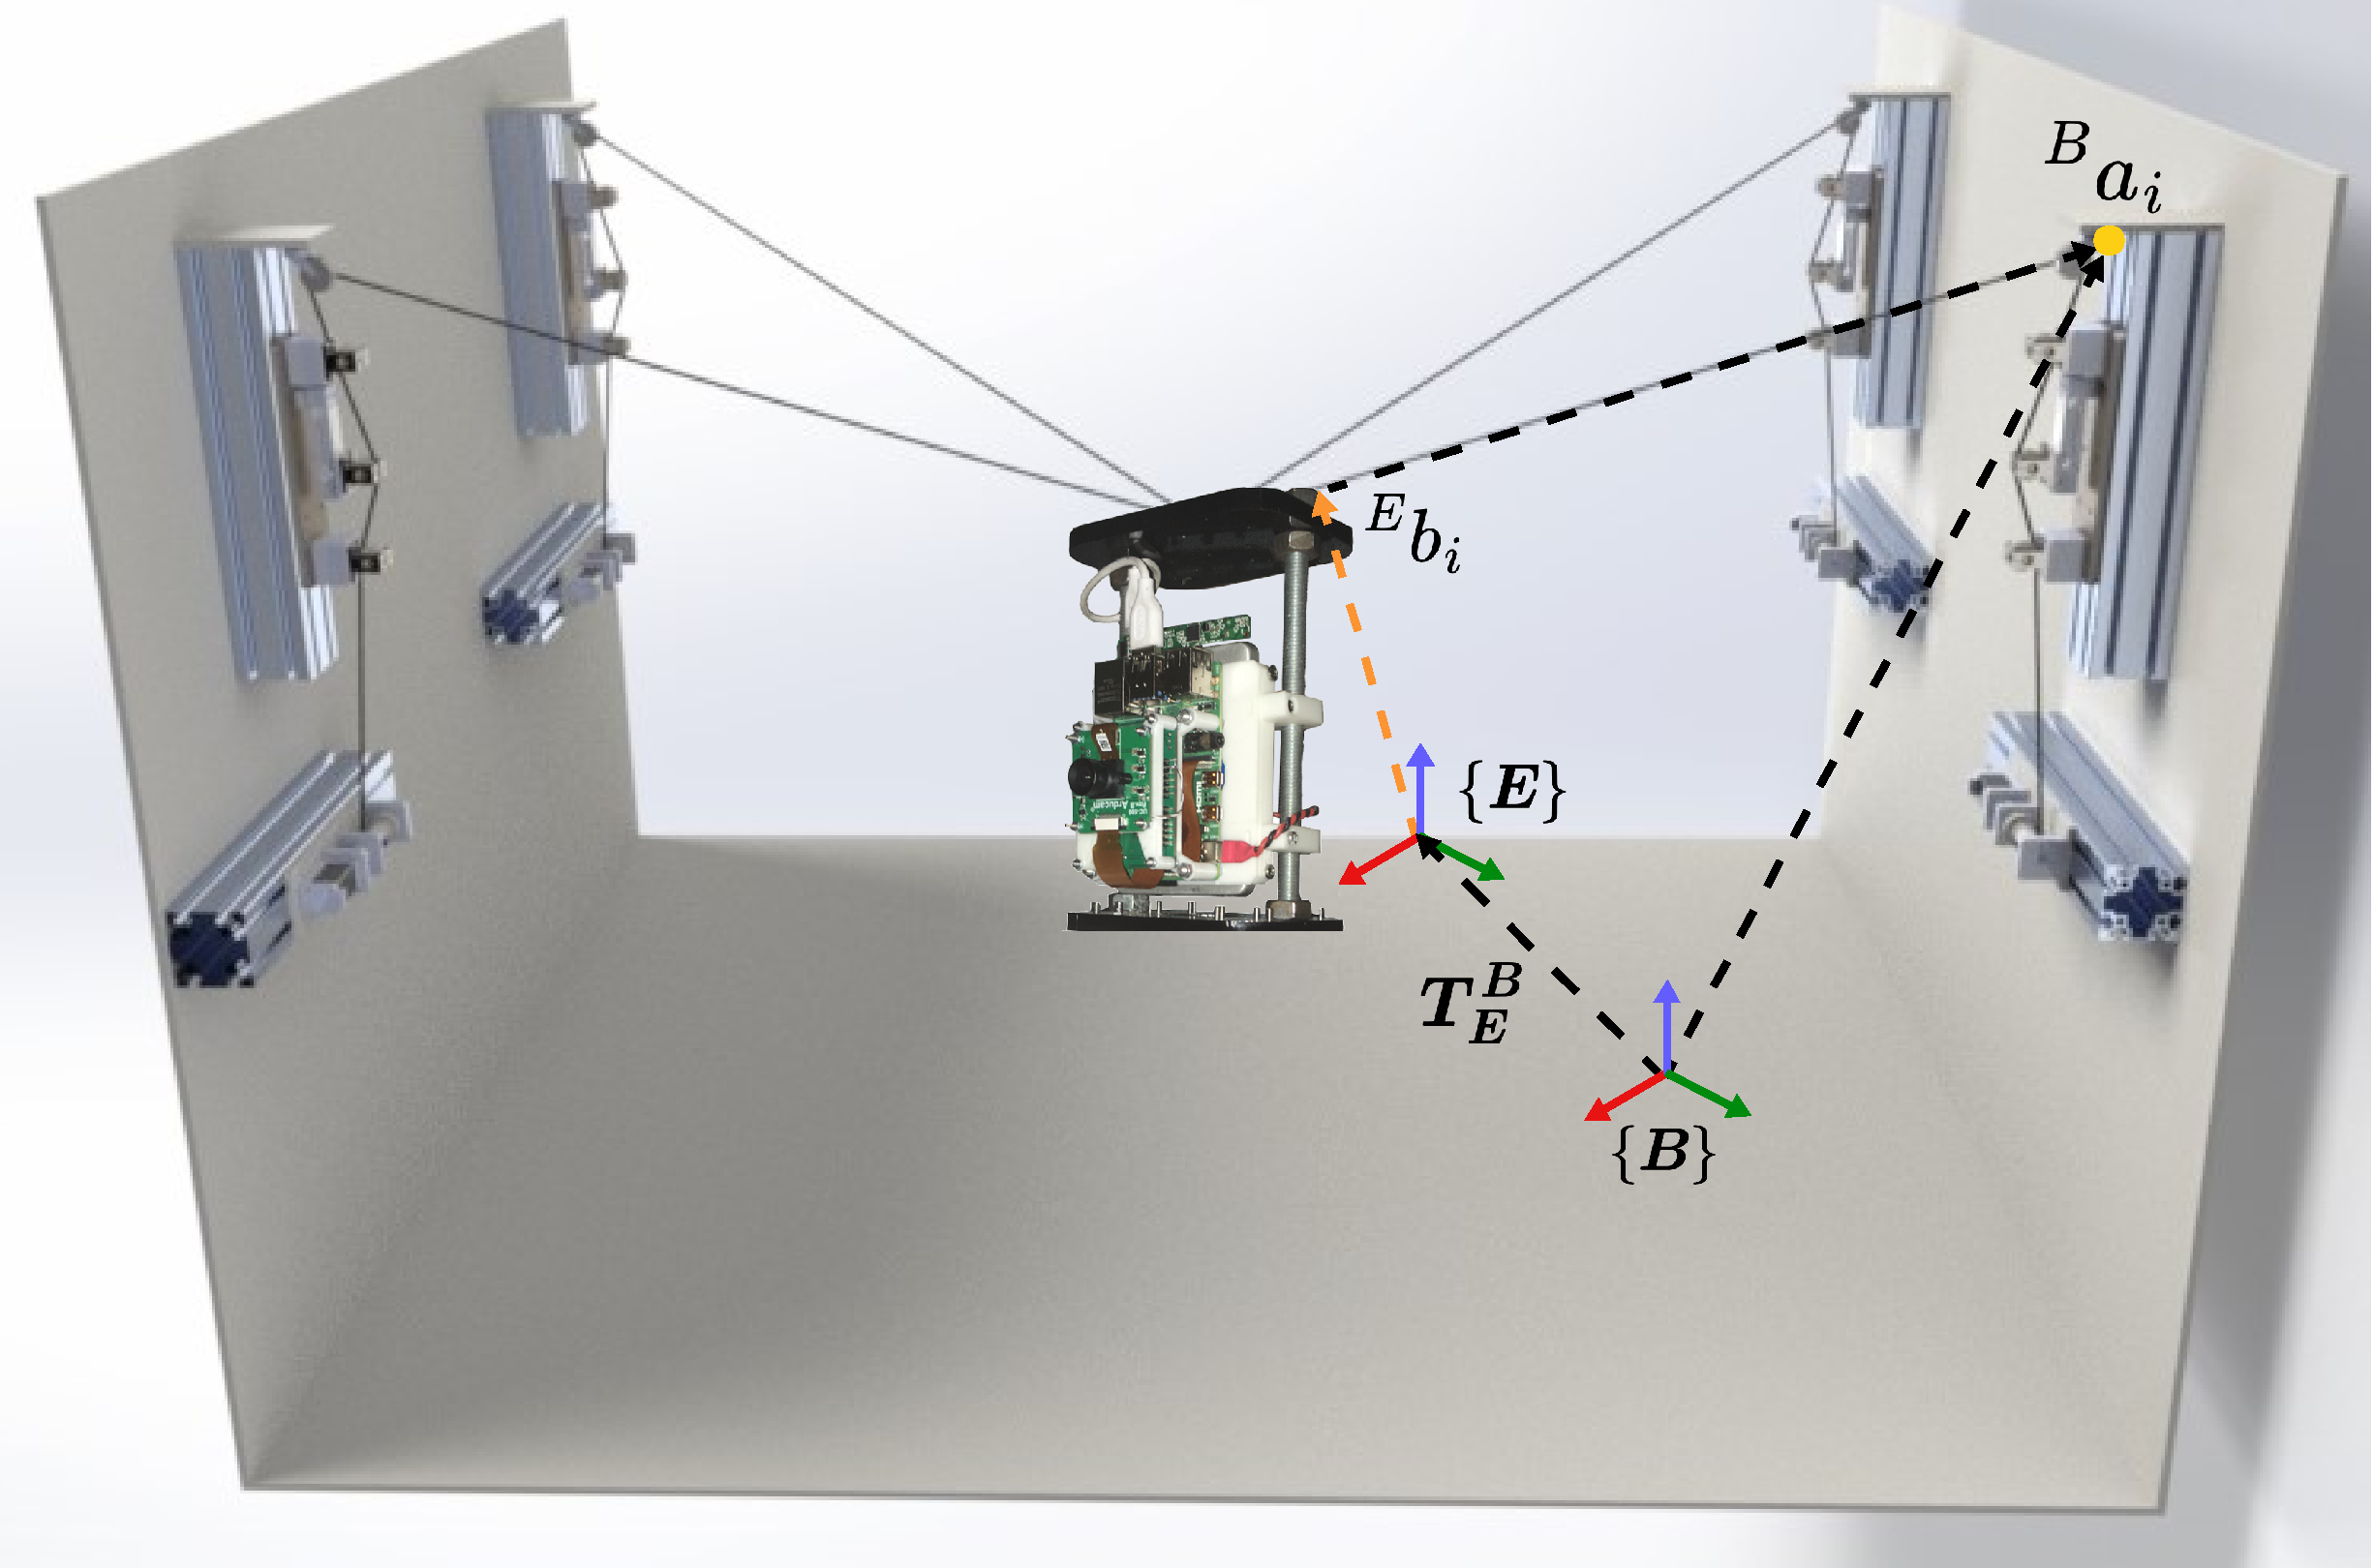
\includegraphics[width=0.5\linewidth]{img/arascam}
	\caption{نمایی از ربات چهار کابلی فروتحریک معلق ARAS-CAM}
	\label{fig:arascam}
\end{figure}

\subsection{بیان فرمول‌بندی مسئله و فرضیات} \label{seq:formulation_rigid}
برای فرمول‌بندی مسئله از هندسه بیان شده در شکل 
\ref{fig:arascam}
استفاده می کنیم. برای یک ربات با کابل‌های صلب، مدل اندازه‌گیری طول کابل \( \hat{z}_i \) با استفاده از حسگر انکودر روی ربات برای نمونه $k$، به صورت زیر می تواند فرمول‌بندی ‌شود:
\begin{equation}\label{eq:cable_length_without_young_module}
	\begin{split}
		l^\star_i [k] &\triangleq \| \boldsymbol{R}^B_E ~ {}^B\!\boldsymbol{b}_i + {}^B\!\boldsymbol{t}_E^B - {}^B\!\boldsymbol{a}_i \|_2 \\
		\hat{z}_i [k] &= l^\star_i [k] + l_{i}^0 + w_{\text{enc}} [k]
	\end{split}
\end{equation}


که در آن
\( (\boldsymbol{R}^B_E, {}^B\!\boldsymbol{t}_E^B) \)
 نشان‌دهنده ماتریس جهت‌گیری و بردار انتقال پنجه در دستگاه مختصات پایه،
\(l_{i}^0  \)
نشان‌دهنده مقدار جابجایی اولیه انکودر، و 
\( w_{\text{enc}} [k] \)
 نشان‌دهنده نویز اندازه‌گیری طول است. اگر انعطاف‌پذیری کابل نیز در نظر گرفته شود، نیروی
\( T_i \)
 در کابل، طول اندازه‌گیری شده کابل را به صورت زیر تغییر می‌دهد:
\begin{equation} \label{eq:cable_length_with_young_module}
	\hat{z}_i [k] = \left(1 - \frac{T_i [k] + w_T [k]}{EA} \right) l^\star_i [k] + l_{i}^0 + w_{\text{enc}} [k]
\end{equation}


که در آن \( E \) مدول یانگ کابل، \( A \) سطح مقطع کابل، و \( w_T [k] \) نویز اندازه‌گیری نیرو است. چنانچه نیروی کابل صفر باشد،
\( T_i [k] = 0 \)، 
در معادله 
\ref{eq:cable_length_with_young_module}
 طول اندازه‌گیری شده توسط انکودر با فاصله واقعی بین \( a_i \) و \( b_i \) مطابقت دارد. با این حال، در پیکربندی‌ای که موتور در محل قفل شده و انکودر مقدار ثابتی را می‌خواند، جابجایی طول به دلیل کشیدگی توسط انکودر دیده نمی‌شود اما نسخه مقیاس‌شده وابسته به نیرو از فاصله واقعی \( l^\star_i [k] \) اندازه‌گیری می‌شود. با افزایش \( E \) (کابل‌های سفت)، اهمیت این مقیاس‌بندی وابسته به نیرو به صفر کاهش می‌یابد و معادله 
\ref{eq:cable_length_with_young_module}
به معادله
\ref{eq:cable_length_without_young_module}
 ساده می‌شود. در مورد ربات‌ با کابل‌های انعطاف‌پذیر، فرض می‌کنیم که حسگرهای نیروی کابل در نزدیکی عملگرها قرار گرفته‌اند. با این حال، برای بسیاری از کاربردها که به ربات‌های کابلی با اندازه متوسط نیاز دارند، انعطاف‌پذیری کابل ممکن است با انتخاب مناسب کابل‌ها قابل صرف نظر باشد.

علاوه بر فرمول‌بندی سینماتیک، مطابق شکل
\ref{fig:arascam}
 ربات با یک دوربین روی انتهای ربات، متصل به پنجه، تجهیز شده است. در اینجا ما تصاویر دریافتی از این دوربین را با استفاده از الگوریتم SVO
\cite{Forster2014ICRA}
  برای تولید اندازه‌گیری‌های مکان ربات در فضای
$SE(3)$
به سیستم وارد می کنیم که بدین‌ترتیب برای مکان‌یابی ربات زنجیره‌ای از تغیرات مسافت‌پیمایی با فرمول بندی زیر به هم وصل می‌شوند:
\begin{equation}
	\Delta \boldsymbol{T}^k_{k-1} = \begin{bmatrix} \boldsymbol{R}^k_{k-1} & \boldsymbol{t}^k_{k-1} \\ \boldsymbol{0} & s^{-1} \end{bmatrix}
\end{equation}

در طول مرحله کالیبراسیون و مکان‌یابی با استفاده از این الگوریتم، فرض می‌کنیم محیط‌ دارای نور خوب با بافت‌های غنی از ویژگی بوده و دوربین به آرامی حرکت می‌کند.  مسئله کالیبراسیون و مکان‌یابی به تخمین مشترک مکان‌های ربات
$\boldsymbol{T}^B_E [k]$,
مکان‌های نقاط اتصال کابل‌ها به پولی‌های متناظر
$\boldsymbol{a}_i$،
 طول‌های اولیه کابل‌ها
$l_{i}^0$،
و مقیاس الگوریتم مسافت‌پیمایی
$s$
با استفاده از اندازه‌گیری‌های الگوریتم مسافت‌پیمایی
 \( \Delta \boldsymbol{T}^k_{k-1} \)،
انکودرهای طول کابل
$z_i [k]$،
و برای ربات‌ها با کابل‌های انعطاف‌پذیر، اندازه‌گیری‌های نیرو 
$T_i$ 
کاهش می‌یابد. این تصویر از تخمین مشترک به حل یک مسئله بهینه‌سازی منجر می‌شود که مدل سینماتیکی را به اندازه‌گیری‌های انجام شده نزدیک‌تر کند. به عبارتی دیگر، فرمول‌بندی که در
 \ref{eq:optimization_equation_conventional_multi_sensor_measurement} 
 ایجاد شد، در اینجا به فرمول‌بندی زیر بازنویسی می‌شود:
\begin{equation}
	\min_{\boldsymbol{a}_i, l_{i}^0, \boldsymbol{T}^B_E [k], s} \sum_k \| h(\boldsymbol{a}_i, l_{i}^0, \boldsymbol{T}^B_E [k], s) - z_i [k] \|^2_2
\end{equation}

که مدل اندازه‌گیری، \( h(.) \)، به صورت زیر تعریف می‌شود:
\begin{equation} \label{eq:mathmatic_model_rigid_cable}
	h(\boldsymbol{a}_i, l_{i}^0, \boldsymbol{T}^B_E [k], s) = s \left( 1 - \frac{T_i [k] + w_T [k]}{EA} \right) l^\star_i [k] + l_{i}^0 + w_{\text{enc}} [k] 
\end{equation}
با این فرمول‌بندی، مقادیر بهینه نقاط پولی‌های ربات
$a_i^*$
و مکان‌های پنجه ربات
$\boldsymbol{t}^{B^{*}}_{E}$
با پارامتر بزرگنمایی
$s$
به دست می‌آید.


\subsection{رویت‌پذیری}
برای تحلیل مشاهده‌پذیری، از روش ارائه شده در
\cite{blueml2021bias}
الهام گرفته‌ایم که از سیستم‌های مکان‌یابی  UWB\footnote{\lr{Ultra Wide Band (UWB)}}
برای مقادیر اولیه الگوریتم بهینه‌سازی خود استفاده کرده‌است. با توجه به مدل اندازه‌گیری در معادله
\ref{eq:cable_length_with_young_module}
، می‌توان مسئله حداقل مربعات را به صورت خطی زیر بازنویسی کرد:
\begin{equation}\label{eq:observibility}
	\begin{bmatrix}
		-2t_x[1]\alpha[1] & \cdots & -2t_x[k]\alpha[k] \\
		-2t_y[1]\alpha[1] & \cdots & -2t_y[k]\alpha[k] \\
		-2t_z[1]\alpha[1] & \cdots & -2t_z[k]\alpha[k] \\
		d^2_t[1]\alpha[1] & \cdots & d^2_t[k]\alpha[k] \\
		2z_i[1] & \cdots & 2z_i[k] \\
		\alpha[1] & \cdots & \alpha[k]
	\end{bmatrix}^T
	\begin{bmatrix}
		s^2 a_x \\
		s^2 a_y \\
		s^2 a_z \\
		s^2 \\
		l_{0_i} \\
		s^2 (d^2_a - l_{0_i}^2)
	\end{bmatrix}
	=
	\begin{bmatrix}
		z_i[1]^2 \\
		z_i[2]^2 \\
		\vdots \\
		z_i[k]^2
	\end{bmatrix}
\end{equation}

که در آن \( d_a \)، \( d_t[k] \) و \( \alpha[k] \) به صورت زیر تعریف می‌شوند:
\begin{equation}
	\begin{split}
		\alpha[k] &\triangleq \left(1 - \frac{\tau_i[k]}{EA}\right) \\
		d^2_t[k] &\triangleq t^2_x[k] + t^2_y[k] + t^2_z[k], \quad d^2_a \triangleq t^2_x + a^2_y + a^2_z
	\end{split}
\end{equation}

همان‌طور که در 
\cite{blueml2021bias}
اشاره شده است، سیستم خطی در معادله 
\ref{eq:observibility}
معمولاً در عمل خوش تعریف\footnote{\lr{well-pose}}
و منجر به پاسخ‌های ضعیف خواهد شد. ما به جای این روش معرفی شده برای نقطه شروع، از چارچوب احتمالی استفاده می‌کنیم تا راه‌حل‌های با کیفیت بالاتری به دست آوریم. با این حال، وجود یک پاسخ برای این سیستم خطی، مشاهده‌پذیری پارامترهای سینماتیکی را با توجه به مجموعه اندازه‌گیری‌های تعریف شده در بخش قبلی اثبات می‌کند.









\section{بهینه‌سازی پارامترها با استفاده از گراف‌های عاملی} \label{seq:factor_graph_for_rigid_cable}

برای حل مسئله مکان‌یابی و کالیبراسیون ربات کابلی ارائه شده در شکل
\ref{fig:arascam}
در ساختار گراف، ما یک گراف عامل با گره‌های متغیر 
$\boldsymbol{X}(k) \in SE(3)$,
$l_{i}^0$,
$T_i(k), S \in \mathbb{R}$ 
و
$\boldsymbol{a}_i, \boldsymbol{b}_i(k) \in \mathbb{R}^3$ 
تعریف می‌کنیم که به ترتیب نمایانگر وضعیت دوربین، انحراف طول کابل (یا طول اولیه کابل)، نیرو‌های کابل، مکان نقاط پولی و نقاط اتصال کابل‌ها بر روی پنجه ربات هستند. شکل 
\ref{fig:rigidcable_factorgraph}
نشان‌دهنده این گراف می باشد. 
\begin{figure}
	\centering
	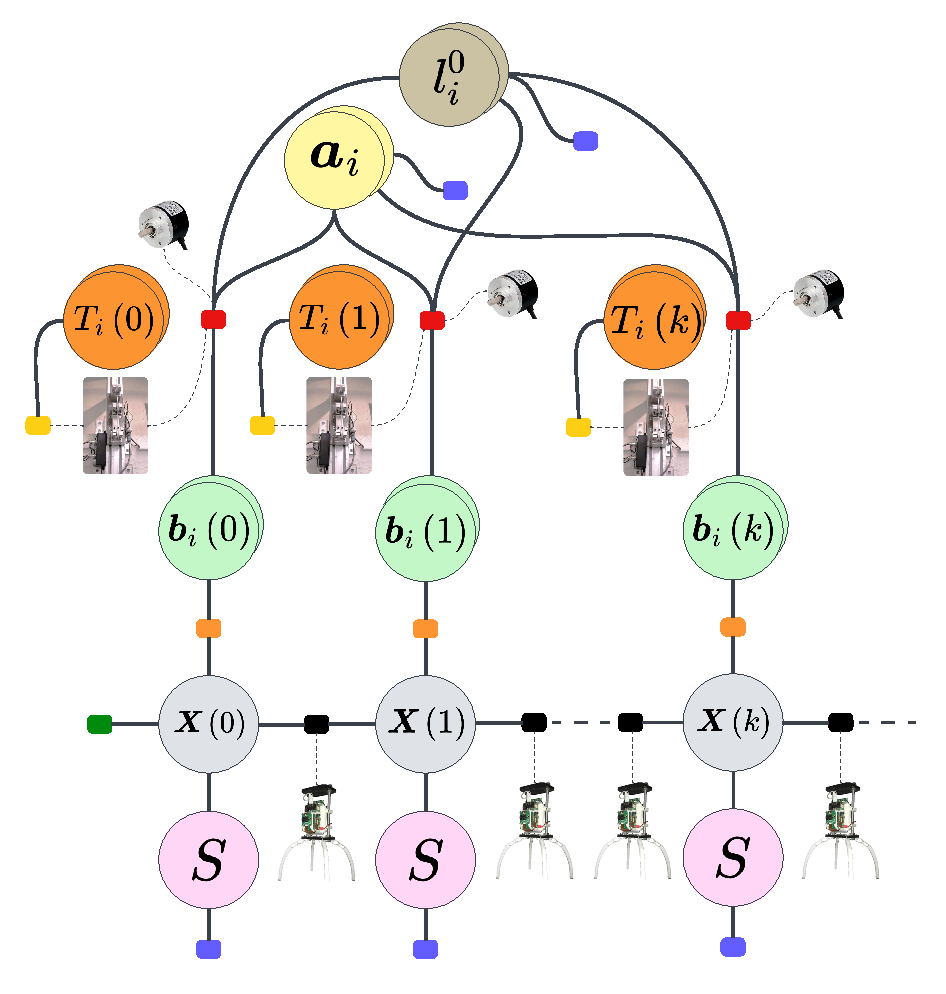
\includegraphics[width=0.6\linewidth]{img/rigidcable_factorgraph}
	\caption{گراف عامل پیشنهادی برای حل مسئله کالیبراسیون و مکان‌یابی ربات کابلی منعطف}
	\label{fig:rigidcable_factorgraph}
\end{figure}


همانطور که در شکل 2 نشان داده شده است، گره‌های
$\boldsymbol{X}(k)$
با عامل‌های مسافت‌پیمایی مقیاس‌بندی شده (نشان داده شده با رنگ سیاه) که نشان‌دهنده مکان‌های نسبی و مقیاس‌دهی مسیر براساس مقدار گره مقیاس 
$S$
 است، به هم متصل می‌شوند. از سوی دیگر، هر وضعیت دوربین 
$\boldsymbol{X}(k)$
 به چهار نقطه اتصال کابل‌های در پنجه ربات
$\boldsymbol{b}_i(k)$
از طریق عامل‌های مکان نسبی (نشان داده شده با رنگ نارنجی) که با تبدیل‌های تعریف شده در مدل CAD پنجه ربات اولیه‌سازی شده‌اند، متصل می‌شود (که مشمول پارامترهای کالیبراسیون در این کار نیستند). هر یک از گره‌های
$\boldsymbol{b}_i(k)$
به نقاط اتصال پولی
$\boldsymbol{a}_i(k)$
از طریق عامل‌های سینماتیکی (نشان داده شده با رنگ قرمز) که طبق بخش 
\ref{seq:formulation_rigid}
 و با استفاده از مدل اندازه‌گیری
\ref{eq:mathmatic_model_rigid_cable}
تعریف شده‌اند، متصل می‌شوند.

همچنین، این عامل‌های سینماتیکی نیز به گره‌های نیروی کابل
$T_i(k)$
و پارامتر متغیر طول اولیه کابل
$l_{i}^0$
 متصل هستند. هر یک از این گره‌های نیرو کابل، توسط عامل‌های پیشین (نشان داده شده با رنگ زرد) با اندازه‌گیری‌های حسگر نیروسنج، محدود شده‌اند. همچنین، با استفاده از عامل پیشین متصل شده به اولین مکان پنجه ربات (نشان داده شده با رنگ سبز)، نقطه صفر مکان‌یابی ربات را می‌توان معین کرد. توجه داشته باشید که برای ربات‌های کابلی که کابل‌های با کیفیت بالا توسعه پیدا کرده‌اند، نیاز به اندازه‌گیری نیروی کابل ممکن است حذف شود و گره‌های
$T_i(k)$
از گراف عاملی حذف شوند. در این حالت، عوامل سینماتیکی باید براساس معادله
\ref{eq:cable_length_without_young_module}
تعریف شوند. 

در نهایت، با انتخاب مقادیر مناسبی برای میانگین و ماتریس‌های گوسی مقادیر اولیه عامل‌های متصل به گره‌های مقایس دهی (در بخش 
\ref{seq:monte_carlo}
روشی برای این انتخاب مناسب ارائه خواهد شد)، محل پولی‌ها و مقادیر اولیه طول کابل‌ها (نشان‌ داده شده با رنگ آبی) که به عنوان پارامترهای کالیبراسیون نقش بازی می کنند، گراف نهایی را تشکیل می‌دهیم. با استفاده از یک حل‌کننده مناسب می‌توان تابع بهینه‌ احتمالاتی نهایی را بهینه کرد. مقادیر گره‌های سینماتیکی بهینه شده و عدم قطعیت‌های به حاشیه رفته مربوطه خروجی نهایی چارچوب ما هستند.

\section{نتایج پیاده‌سازی}
این بخش به ارزیابی کاربردی بودن گراف پیشنهادی در تخمین مشترک پارامترهای سینماتیک و مکان‌های پنجه ربات، مستقل از دستگاه‌های اندازه‌گیری خارجی یا مقادیر اولیه پارامترها می‌پردازد. علاوه بر این، مزایای ترکیب بینایی-سینماتیک\footnote{\lr{Visual-Kinematic Fusion (VK-F)}}
 نیز در این بخش مورد بررسی قرار می‌گیرد.

\subsection{راه‌اندازی سیستم و فرضیات}
ما آزمایشات خود را با استفاده از ربات ARAS-CAM، یک ربات کابلی با اندازه متوسط و مساحت کاری 7 × 3 × 4 مترمکعب که توسط گروه رباتیک ARAS در دانشگاه صنعتی خواجه نصیرالدین طوسی توسعه داده شده است، انجام می‌دهیم.این ربات، به یک مجموعه کامل از حسگرهای سینماتیک و بینایی-اینرسی\footnote{\lr{Visual-Inertial (VI)}}
 مجهز شده است تا تحقیقات برآورد حالت برای ربات‌های کابلی را ممکن سازد. به طور خاص، هر واحد عملگر کابلی به یک حسگر نیرو و یک انکودر اندازه‌گیری طول نسبی مجهز شده است. از سوی دیگر، پنجه ربات دارای یک سیستم تعبیه شده با دوربین تک‌چشمی OV9281\footnote{\lr{monocular camera}}
 و واحد اندازه‌گیری اینرسی BMI088 است. برای پیش‌برد اهداف تحقیقات، 12 رشته داده با اندازه‌گیری‌های داده مرجع سه‌بعدی با استفاده از سیستم ردیابی مکانی توسعه یافته در این آزمایشگاه، از این ربات با عنوان مجموعه داده ARAS-CAM ضبط کرده‌ایم. برای پیاده‌سازی‌های انجام شده، ما از رشته داده 01 این مجموعه به عنوان نماینده حرکات پویاتر و از رشته داده 12 به عنوان یک همتای هموارتر استفاده می‌کنیم.

به دلیل اندازه متوسط ARAS-CAM و انتخاب کابل‌های کولار بسیار سخت، تقریب کابل بدون جرم که پیش‌تر مورد بحث قرار گرفت، در تمام آزمایشات ما حفظ می‌شود. علاوه بر این، فرض می‌کنیم که تقریب طول کابل اولیه در محدوده 
$\pm~50$
سانتی‌متر مقدار واقعی قرار دارند که در عمل با آزاد کردن کابل‌ها از یک پیکربندی اولیه شناخته شده قابل دستیابی است.

برای تولید اندازه‌گیری‌های بینایی حرکتی، از الگوریتم SVO
\cite{Forster2014ICRA}
استفاده شده است که از نظر محاسباتی کارآمد بوده و به طور گسترده در کاربردهایی از جمله پرواز خودران تا واقعیت مجازی مورد استفاده قرار می‌گیرد. ما از اندازه‌گیری‌های مرجع برای اندازه‌گیری عدم قطعیت بینایی حرکتی الگوریتم SVO در پیاده‌سازی خود استفاده می‌کنیم.

\subsection{کالیبراسیون خودکار بدون پارامترهای اولیه} \label{seq:monte_carlo}
برای راه‌اندازی گراف فرمول‌بندی شده، باید حدس نسبتا مناسبی از مقادیر اولیه پارامتر‌های شناسایی و ماتریس‌های کوواریانس نویز در دست داشته باشیم.روشی که برای دستیابی به این موارد معرفی می کنیم، الگوریتمی مبتنی بر روش مونت-کارلو می باشند. این الگوریتم و نحوه کارکرد آن به صورت مفصل در 
\cite{khorrambakht2023graph}
توضیح داده شده است. در این بخش، ما از این الگوریتم ابتدایی مونت-کارلو برای شناسایی مکان‌های نقاط پولی، مقادیر اولیه طول کابل، و مقیاس بینایی حرکتی استفاده می‌کنیم. پس از شروع کارکرد SVO، کاربر یک چارچوب مختصات صفر اختیاری با قرار دادن انتهای ربات در آن حالت و شروع الگوریتم انتخاب می‌کند. سپس، انتهای ربات بر اساس جهت عدم قطعیت بیشتر یا با دنبال کردن هنجار حرکت انتهای ربات در امتداد سه محور انتقالی و پوشش حجم بزرگ حرکت می‌کند.

\begin{figure}
	\centering
	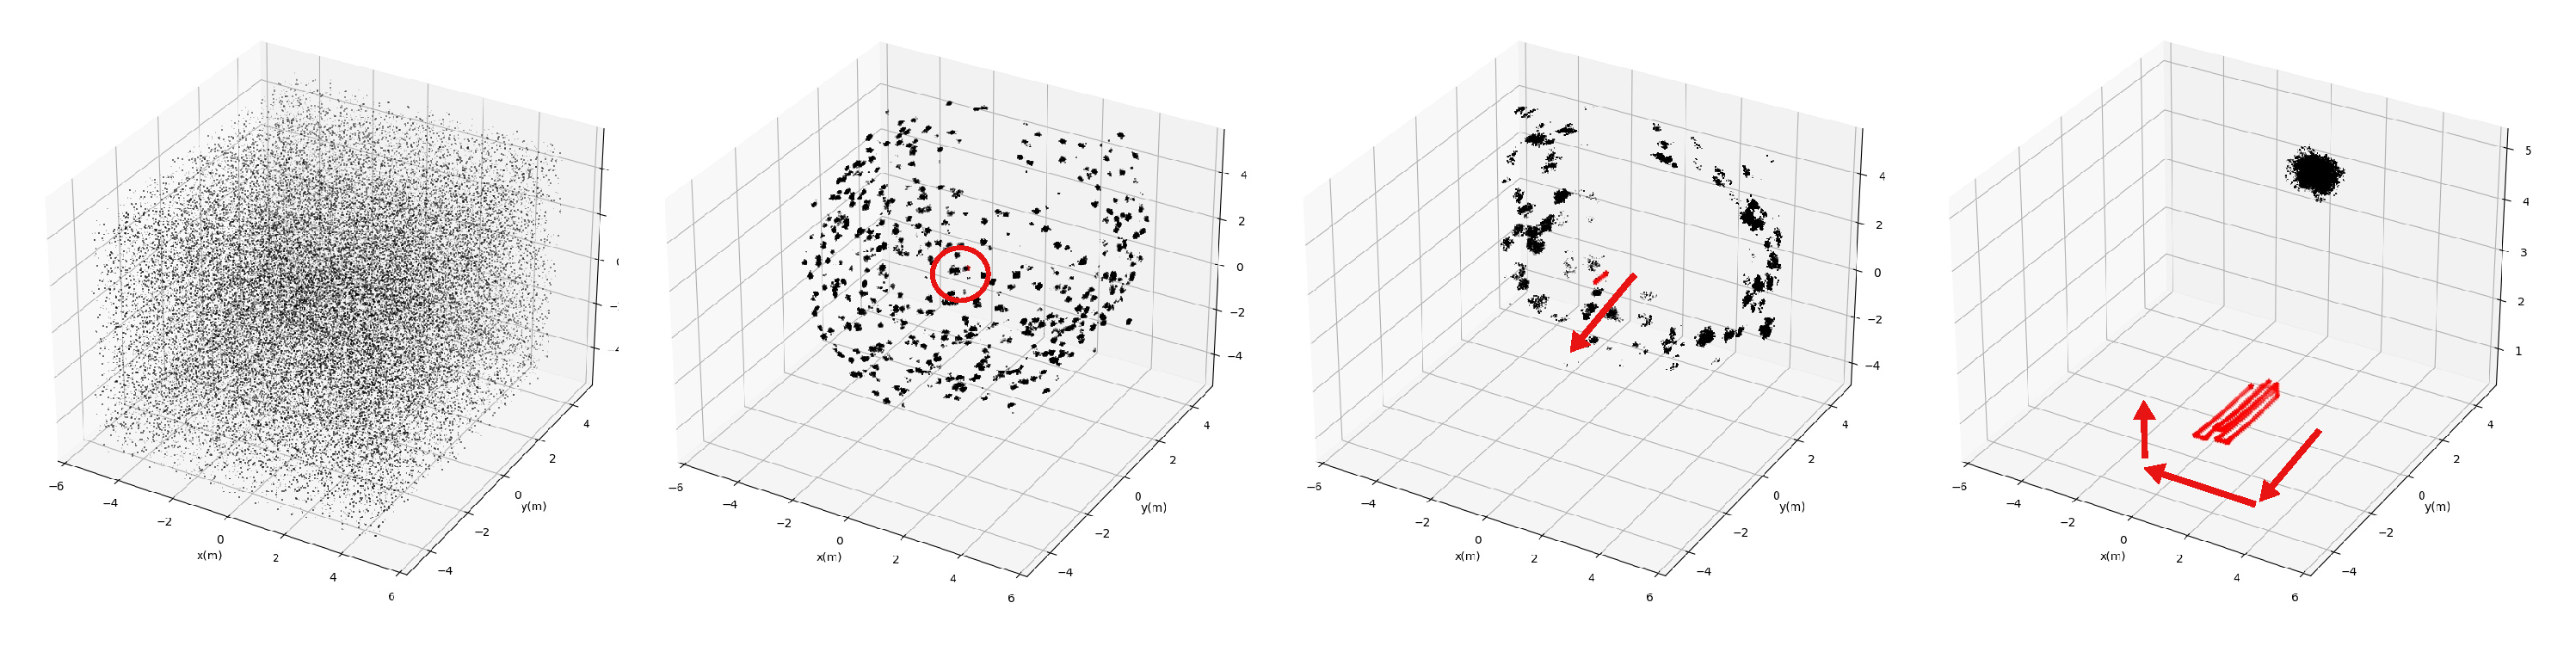
\includegraphics[width=1\linewidth]{img/monte_carlo}
	\caption{پالایش متوالی یک باور یکنواخت بر روی پارامترهای سینماتیکی از طریق الگوریتم مونت-کارلو}
	\label{fig:montecarlo}
\end{figure}

همانطور که در شکل 
\ref{fig:montecarlo}
نشان داده شده است، در ابتدا وقتی اطلاعاتی به فیلتر تزریق نمی‌شود، ذرات به طور یکنواخت در منطقه پخش می‌شوند(اولین نمودار از چپ). اما، همانطور که در شکل (نمودار دوم از چپ) نشان داده شده است، پس از کمی حرکت دادن دوربین در طول یک خط مستقیم، توزیع یکنواخت به یک پوسته کروی تبدیل می‌شود که تمامی مکان‌های ممکن برای مکان پولی را نشان می‌دهد و ضخامت آن عدم قطعیت بر طول اولیه کابل را نشان می‌دهد. به تدریج، با حرکت طولانی‌تر انتهای ربات و در امتداد جهت‌های دیگر، کره به یک حلقه تبدیل می‌شود همانطور که در شکل (نمودار سوم از چپ) نشان داده شده است. در نهایت به یک خوشه بیضوی از ذرات که مکان شناسایی شده نقطه پولی و عدم قطعیت مربوطه آن را نشان می‌دهد تبدیل می‌شود که در شکل (نمودار چهارم از چپ) نشان داده شده است.

\subsection{ترکیب بینایی-سینماتیک و استفاده از گراف عامل معرفی شده}
در این بخش، ما گراف عامل را که در بخش 
\ref{seq:factor_graph_for_rigid_cable}
 بیان شده است، پیاده‌سازی می‌کنیم تا پارامترهای مراحل قبل را با در نظر گرفتن تأثیر متقابل تمام حالت‌ها بهبود دهیم. ما این گراف عامل را با استفاده از کتابخانه GTSAM
\cite{dellaert2012factor}
 که یک حل‌کننده معروف در جامعه SLAM است و حالت‌های اجرای افق متحرک و افزایشی بسیار کارآمدی دارد، پیاده‌سازی می‌کنیم. گراف‌های عامل این گراف به صورت دستی در کلاس‌های C++ نوشته شده و به حل‌کننده این کتابخانه متصل شده‌است. 
 
\begin{table}[!t]
	\small
	\centering
	\caption{خطای مکان‌یابی با روش‌های مختلف (واحد متر)}
	\label{tab:calibration_results}
	\renewcommand{\arraystretch}{1.0} % Increase row spacing Me?
	\footnotesize
	\begin{tabular}{c|c|c|c}
		\toprule
		\rowcolor{gray!10}
		\hline
		\text{رشته} & \rl{خطای MSE سیتنماتیک مستقیم} & \rl{خطای MSE بینایی حرکتی} &  \rl{خطای MSE روش پیشنهادی}\\
		\midrule
		$01$ &  $0.036$ &  $0.05$  &   $0.029$ \\
		\hline
		$12$ &  $0.035$  &  $0.03$  &   $0.028$ \\
		\hline
		$\textbf{میانگین}$ &  $0.0355$ & $0.04$ & $0.0285$ \\
		\bottomrule
	\end{tabular}
\end{table}
 
 
مزایای ترکیب سینماتیک و حسگر بینایی در بهبود نتایج نقش موثری داشته است.جدول 
\ref{tab:calibration_results}
خلاصه‌ای از این نتیجه را در هر حالت ارائه می‌دهد. همانطور که انتظار می‌رود، دقت کلی با ترکیب این دو حالت بهبود می‌یابد. به ویژه برای رشته داده 01، ترکیب بینایی-سینماتیک به بهبود دقت 23 درصدی در مقایسه با سینماتیک مستقیم و 72 درصدی در مقایسه با بینایی حرکتی منجر می‌شود. این اعداد به ترتیب برای رشته داده 12 برابر با 25 درصد و 7 درصد است. بهبود عملکرد در رشته داده 01 بیشتر است، که با این واقعیت همخوانی دارد که انتهای ربات در این رشته داده حرکات پویاتری دارد و در نتیجه بینایی حرکتی در معرض تخریب بیشتری قرار می‌گیرد. از سوی دیگر، این حرکات پویا نوسانات بزرگی ایجاد می‌کنند که از حالت‌های سینماتیک قابل مشاهده نیستند و منجر به خطاهای نسبتاً بزرگی می‌شوند که در
\cite{allak2022kinematics}
نیز نشان داده شده است.







در ادامه، کاهش خطای پنجه ربات را پس از بهبود پارامترهای اولیه بررسی می‌کنیم. این خطا را به عنوان میانگین مربع خطا بین طول کابل محاسبه شده از معادله 
\ref{eq:cable_length_without_young_module}
 و مقادیر داده‌های انکودر از ربات تعریف می‌کنیم. ما از این خطا به عنوان یک معیار جانشین برای مکان‌های نقاط پولی استفاده می‌کنیم زیرا در پیاده‌سازی ما، قرقره‌ها در خارج از میدان دید سیستم ردیابی ما (سیستم داده‌های مرجع\footnote{\lr{Ground Truth (GT)}}
 ) قرار دارند و بنابراین مقادیر واقعی متناظر در نسخه فعلی مجموعه داده در دسترس نیستند. 
 
 \begin{figure}
 	\centering
 	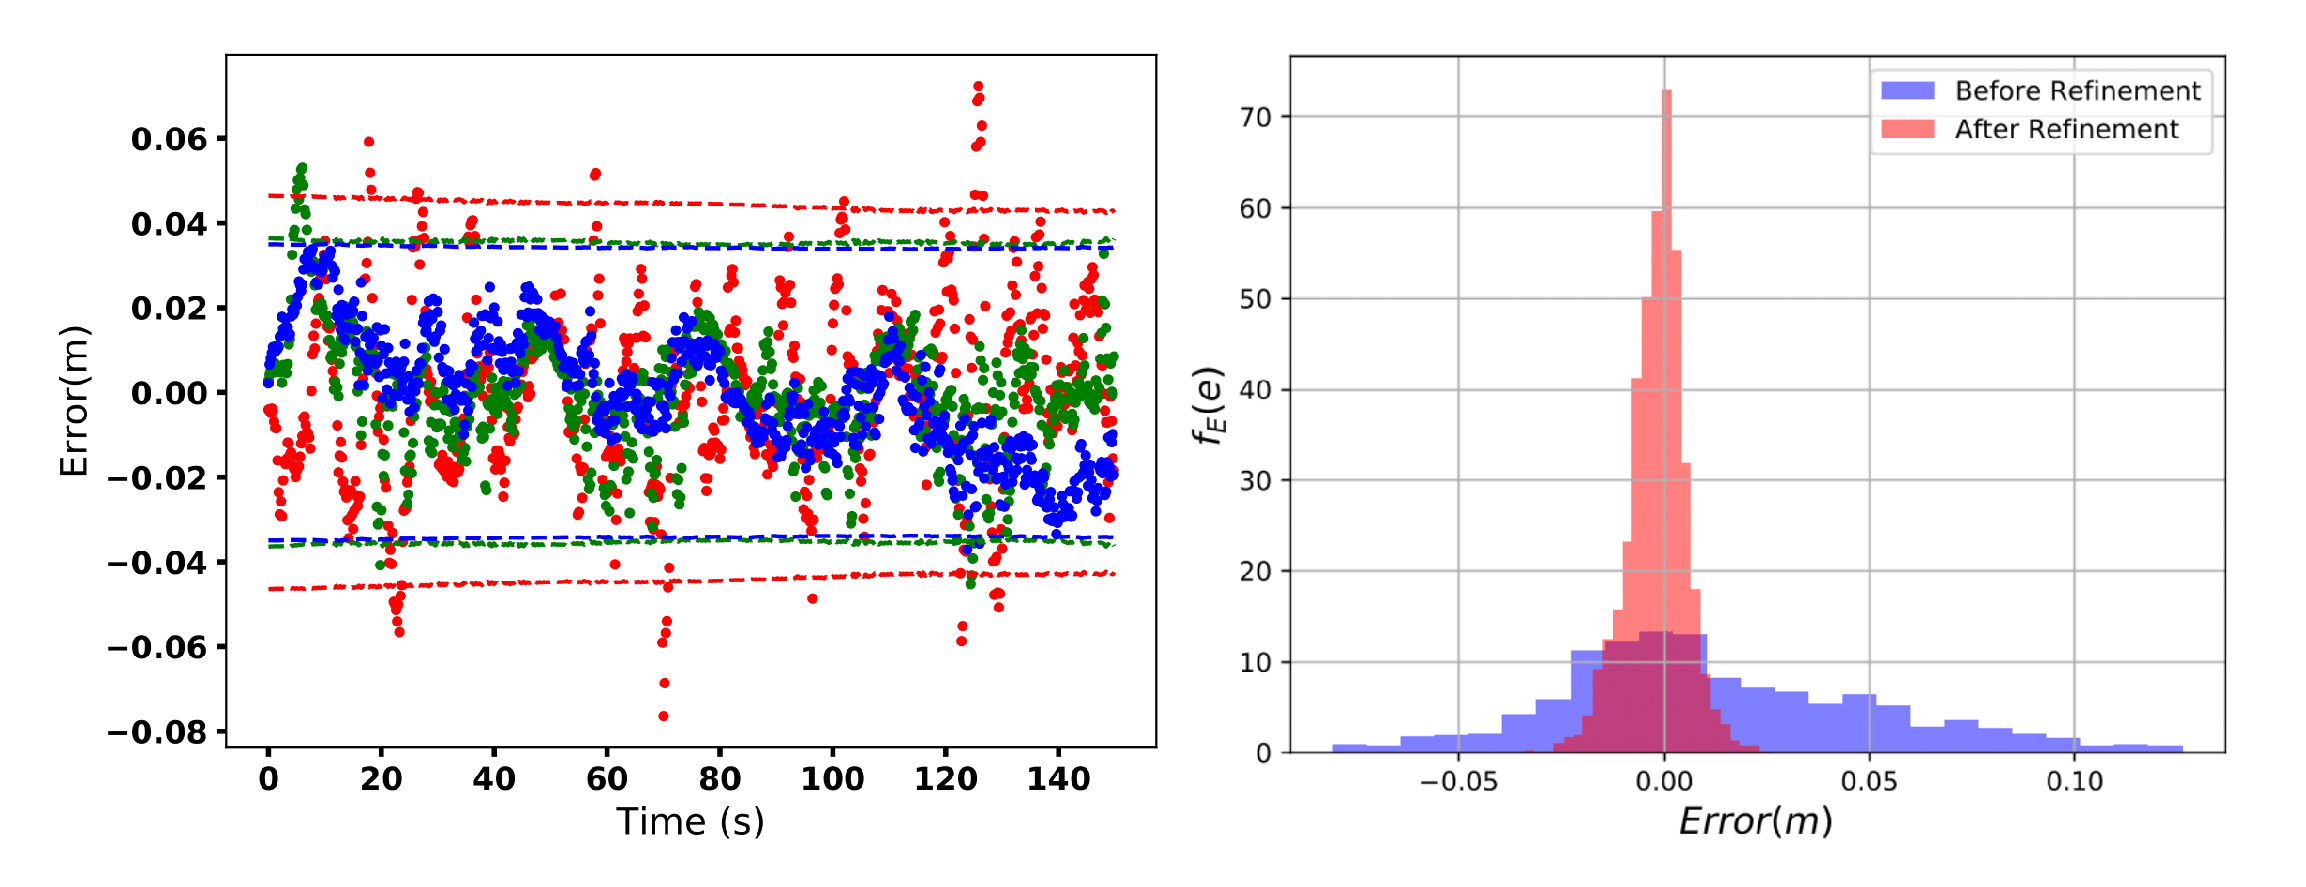
\includegraphics[width=0.9\linewidth]{img/calibration_result_rigid}
 	\caption{ راست: توزیع خطای پنجه قبل و بعد از بهبود پارامترها، چپ: خطای مکان‌یابی در دستگاه کارتزین}
 	\label{fig:calibrationresultrigid}
 \end{figure}
 
 شکل 
 \ref{fig:calibrationresultrigid}
 (نمودار سمت راست)
 توزیع خطای پنجه ربات را قبل و بعد از بهبود پارامترها نشان می‌دهد. همان‌طور که دیده می‌شود، میانگین و واریانس این خطا به طور قابل‌توجهی پس از بهبود کاهش یافته است. به طور خاص، برای رشته داده 01، مقدار خطا قبل از بهبود $0.043$ متر و پس از بهبود $0.0049$ متر است که نشان‌دهنده یک کاهش مرتبه‌ای در خطا است. این مقادیر برای رشته داده 12 به ترتیب $0.03$ متر قبل و $0.0053$ متر بعد از بهبود هستند. همچنین شکل 
  \ref{fig:calibrationresultrigid}
  (نمودار سمت چپ)
  نشان‌دهنده خطای مکان‌یابی پنجه ربات در دستگاه کارتزین در واحد متر می‌باشد. این خطا بیانگر اختلاف مقادیر مکان پنجه در سه جهت از حل گراف عامل نسبت به مقادیر داده‌های مرجع می‌باشد.

در نهایت، نتایج کیفی اجرای الگوریتم ما بر روی رشته داده 01 در شکل 
\ref{fig:trajectoryandpullyinrigidcable} 
نشان داده شده است. در این شکل، مسیر سیاه رنگ نمایانگر داده‌های مرجع و نقاط قرمز نشان‌دهنده مکان‌های اصلاح شده ربات توسط الگوریتم ما هستند. علاوه بر این، ستاره‌های آبی در شکل مکان‌های پولی قبل از بهبود و دایره‌های قرمز، آن‌ها را پس از بهینه‌سازی مشترک گراف عامل را نشان می‌دهند.

\begin{figure}
	\centering
	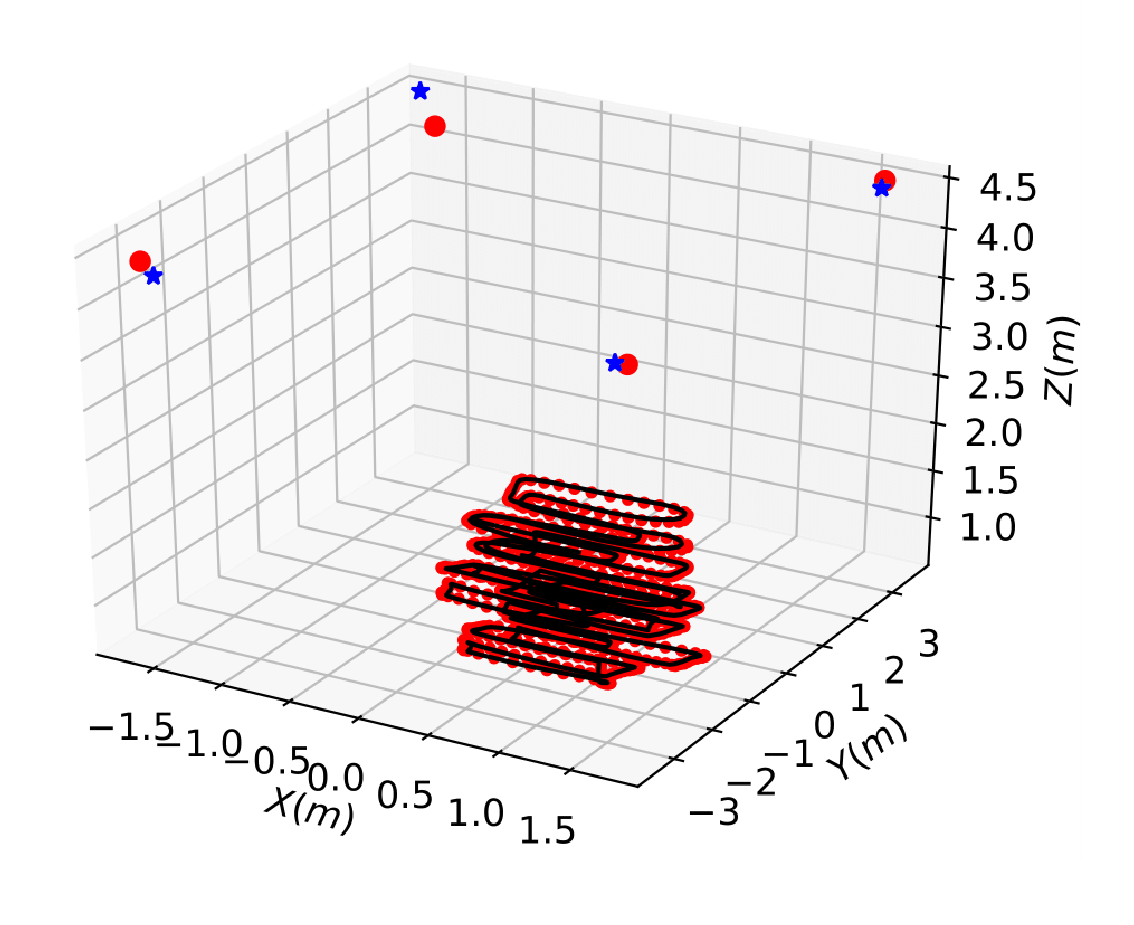
\includegraphics[width=0.5\linewidth]{img/trajectory_and_pully_in_rigid_cable}
	\caption{مسیر طی شده توسط ربات در کنار مکان اولیه و نهایی(بهبودیافته) پولی‌ها}
	\label{fig:trajectoryandpullyinrigidcable}
\end{figure}


\subsection{انتشار عدم قطعیت}
یکی از مزایای چارچوب پیشنهادی، توانایی آن در حفظ و در نظر گرفتن عدم قطعیت و نویز حسگر در طول فرآیند تخمین است. در پیاده‌سازی‌های ما، از مقادیر میانگین و ماتریس‌های کواریانس از برای راه‌اندازی الگوریتم با مقید کردن گراف عامل با استفاده از عامل‌های پیشین استفاده می‌کنیم. نتیجه این کار شباهت عدم قطعیت نهایی گراف عامل به توزیع خطای واقعی است.
ما این سازگاری را با تعیین درصد مقادیر خطا در محدوده‌های $\sigma$، $2\sigma$ و $3\sigma$ بررسی می‌کنیم.

 همانطور که در جدول 
\ref{tab:uncertainty_consistency}
 نشان داده شده است، تقریباً 60 درصد از خطاها در محدوده $\sigma$، 90 درصد در محدوده $2\sigma$ و تقریباً 98 درصد در محدوده $3\sigma$ قرار دارند.
نتایج جدول 
\ref{tab:uncertainty_consistency}
 نزدیک به محدوده‌های تئوریکی $\sigma$ هستند اما نشان‌دهنده یک پاسخ کمی بیش از حد مطمئن است. باید توجه داشت که سازگاری به شدت به مدل‌های حسگر مفروض و همچنین عدم قطعیت بینایی حرکتی تجربی برای الگوریتم SVO وابسته است. ما بررسی دقیق‌تر سازگاری عدم قطعیت را به کارهای آینده موکول می‌کنیم.

\begin{table}[!t]
	\small
	\centering
	\caption{سازگاری آماری عدم قطعیت‌های تخمین زده شده}
	\label{tab:uncertainty_consistency}
	\renewcommand{\arraystretch}{1.0} % Increase row spacing Me?
	\footnotesize
	\begin{tabular}{c|c|c|c}
		\toprule
		\rowcolor{gray!10}
		\hline
		\text{محور} & \rl{$\sigma$} & \rl{$2\sigma$} & \rl{$3\sigma$} \\
		\midrule
		$x$ &  $53\%$ &  $82\%$  &   $95\%$ \\
		\hline
		$y$ &  $71\%$  &  $92\%$  &   $97\%$ \\
		\hline
		$z$ &  $51\%$ & $88\%$ & $99\%$ \\
		\bottomrule
	\end{tabular}
\end{table}


\section{بحث و گفت‌وگو}
روش پیشنهادی در این فصل یک دیدگاه منعطف و یکپارچه در مورد کالیبراسیون و برآورد حالت برای ربات‌های کابلی منعطف در راستای طول کابل، ارائه می‌دهد. این یکپارچگی در جامعه SLAM به شکل اجرای موازی تنظیم مجموعه\footnote{\lr{Boundle Adjustment (BA)}}
 و ردیابی دوربین\footnote{\lr{camera tracking}}
 به خوبی شناخته شده است. به ویژه برای عملکرد بلادرنگ\footnote{\lr{real time}}
 ، مرحله گراف عامل الگوریتم ما ممکن است به صورت افق متحرک حل شود و حالت‌های قدیمی به فاکتورهای پیشین حاشیه‌سازی شوند. از سوی دیگر، کالیبراسیون اولیه ممکن است بدون محدودیت بلادرنگ و با استفاده از اجرای دسته‌ای گراف روی رشته داده طولانی‌تری انجام شود.

پیاده‌سازی فعلی ما در Python روی یک لپ‌تاپ شخصی با پردازنده Intel Core-i7 و 16 گیگابایت RAM کمتر از یک دقیقه برای هر کابل زمان می‌برد تا روش ابتدایی مونت-کارلو را اجرا کند (برای 750 وضعیت دوربین و 5000 ذره) و حدود 30 ثانیه زمان برای بهبود آن‌ها توسط گراف عامل. حالت‌های اجرای افق متحرک حل‌کننده‌های بسیار کارآمد برای گراف‌های عامل مانند 
\cite{dellaert2012factor} و \cite{martiros2022symforce}
 از جامعه SLAM می‌توانند فرکانس برآورد مکان را به نرخ فریم دوربین افزایش دهند که برای بیشتر کنترل‌کننده‌های حلقه خارجی مناسب است. ما بررسی بیشتر عملکرد بلادرنگ الگوریتم خود را به کارهای آینده موکول می‌کنیم.

یکی دیگر از جنبه‌های مهم الگوریتم پیشنهادی، ماژولار بودن آن است. به ویژه، این فرمول‌بندی اجازه می‌دهد تا دیگر حالت‌ها از جمله اما نه محدود به IMU UWB، و حسگرهای سیستم به راحتی به گراف عامل اضافه شوند. علاوه بر این، اندازه‌گیری‌های شبه‌هندسی مانند هم‌سطحی نقاط پولی (به عنوان مثال دو پولی در همان دیوار) یا فاصله بین مکان‌های پولی (قابل اندازه‌گیری با استفاده از ابزارهای اندازه‌گیری کم‌هزینه) به راحتی در مسئله گنجانده ‌شوند که به طور قابل‌توجهی به دقت کلی تخمین کمک می‌کند.

در نهایت، سیستم پیشنهادی ممکن است به طور مستقیم برای کالیبراسیون سیستم‌های مکان‌یابی UWB استفاده شود. در این سیستم‌ها، مدل اندازه‌گیری فاصله بین تگ و لنگرها دقیقاً با مدل کابل بدون جرم منعطف در نظر گرفته شده در این فصل یکسان است. ما قصد داریم این موضوع را به عنوان کارهای آینده بیشتر بررسی کنیم.


\section{نتیجه‌گیری}

در این فصل، ما پیشنهاد دادیم که از ترکیب داده‌های دوربین و حسگرهای سینماتیکی موجود در ربات به منظور ایجاد یک چارچوب تلفیق آماری برای کالیبراسیون و مکان‌یابی ربات‌های کابلی استفاده شود. این هدف با فرمول‌بندی یک الگوریتم مونت-کارلو که نمایشی از مسئله در ساختار گراف عامل را مقداردهی اولیه می‌کند، محقق شد. رویکرد ما نیازی به استفاده از نشانگرهای خاص نداشت و به جای آن، از راه‌حل‌های عمومی‌تر SLAM برای تخمین حرکت پنجه ربات استفاده کرد. از طریق آزمایش‌های عملی با استفاده از یک مجموعه داده واقعی که توسط ربات \lr{ARAS-CAM} ضبط شده بود، ما عملکرد این رویکرد را ارزیابی کردیم و نشان دادیم که تلفیق داده‌ها باعث افزایش دقت شده و همچنین امکان شناسایی پارامترهای سینماتیکی بدون نیاز به فرضیات اولیه قوی را فراهم می‌کند. 
		% فصل چهارم: نتایج
% !TeX root=../main.tex
\chapter{پیاده سازی رویکرد مبتنی بر گراف جهت مکان‌یابی و کالیبراسیون همزمان برای ربات هایی با کابل های شکم داده}
%\thispagestyle{empty} 
این پایان‌نامه به بررسی دقیق رویکردهای مختلف در حوزه رباتیک برای فرمول‌بندی ریاضی یک مسئله بهینه‌سازی مقید پرداخته است. از تحلیل مزایا و معایب روش‌های مرسوم تا رویکردهای جدید مبتنی بر گراف، روشی جامع برای فرمول‌بندی و حل مسئله بهینه‌سازی کالیبراسیون و مکان‌یابی همزمان ربات‌ها ارائه شده است. در فصل گذشته، عملکرد این روش بر روی یک ربات کابلی مقید که کابل‌های آن به صورت منعطف در نظر گرفته شده بود، ارزیابی شد. پس از معرفی فرمول‌بندی سینماتیکی، گراف مربوط به آن ساخته و نتایج پیاده‌سازی بررسی شد. آنچه از ابتدای این پایان‌نامه به عنوان هدفی مهم معرفی گردید، ماژولاریتی و انعطاف‌پذیری روش، با قیدهای متفاوت و گسترده بود. انتخاب ربات کابلی به عنوان مورد مورد مطالعه، نیز به دلیل امکان پیاده‌سازی و ارزیابی همین هدف بوده است.

در این فصل، بدون تغییر در فرمول‌بندی‌های ارائه شده در فصل قبل، به مسئله قیدهای دینامیکی کابل افزوده خواهد شد. علیرغم پیچیدگی این مدل‌ها، حل‌کننده همچنان با دقت و سرعت بالا به نتایج مطلوب دست خواهد یافت. تاکنون تحقیقات بسیاری بر مدل‌سازی کابل‌های شکم‌دار انجام شده است که نتایج دقیقی به دست داده‌اند. ما نیز برای حل مسئله کالیبراسیون و مکان‌یابی نیازمند افزودن این قیدها به مسئله هستیم. با این حال، پیچیدگی‌های این مدل‌ها باعث شده است که در برخی کارهای اخیر به جای حل مستقیم مسئله با این معادلات، از شبکه‌های عمیق استفاده شود که به دلیل مشکلات خاص خود، دقت و اطمینان کافی ندارند.

روش ما برای حل این چالش، استفاده از همان مقیدسازی‌هایی است که برای کابل‌های منعطف انجام شده بود. در پایان، با حل این مسئله، مزایای این رویکرد را بار دیگر خواهیم دید؛ رویکردی که با دقت و قدرت بالا، مسئله کالیبراسیون و مکان‌یابی همزمان ربات‌ها را، حتی در شرایطی که کابل‌ها بدون جرم نیستند، به نحوی که حل آنها در روش‌های مرسوم دشوار است، به سرانجام می‌رساند.



\section{نمادها و تعاریف} \label{subsec:Assm}
این فصل یک ربات موازی کابلی معلق با شش درجه آزادی ($m=6$) و چهار کابل فعال ($n=4$) را مورد بررسی قرار می‌دهد. از آنجایی که $m>n$، این ربات فروتحریک\footnote{underactuated}
 است و یک ساختار نامقید\footnote{under-constrained}
تشکیل می‌دهد~\cite{ida2021natural}. 
شکل~\ref{fig:frame_robot} ساختار این ربات را نشان می‌دهد که برای وضوح بیشتر تنها یک کابل در آن نمایش داده شده است. 
دستگاه‌مختصات $\mathcal{L}$ به بدنه متحرک ربات متصل است، در حالی که دستگاه‌مختصات جهانی $\mathcal{G}$ به طور ثابت به پایه ربات متصل شده است. مکان پنجه ربات نسبت به دستگاه‌مختصات جهانی با
 $(\bm{p},\bm{R}) \in SE(3)$
نشان داده می‌شود، که در آن
 $\bm{p} \in \mathbb{R}^3$
بردار انتقال از $\mathcal{G}$ به $\mathcal{L}$ است و
 $\bm{R} \in SO(3)$
جهت‌گیری $\mathcal{L}$ نسبت به $\mathcal{G}$ است. کابل $i$ از پایه ربات در نقطه $\bm{p}_{a_i}$ که در دستگاه‌مختصات جهانی تعریف شده است، جدا می‌شود و به پنجه ربات در نقطه $\bm{p}_{b_i}$ که در دستگاه‌مختصات بدنه محلی بیان شده است، متصل می‌شود.

\begin{figure}[t]
	\centering
	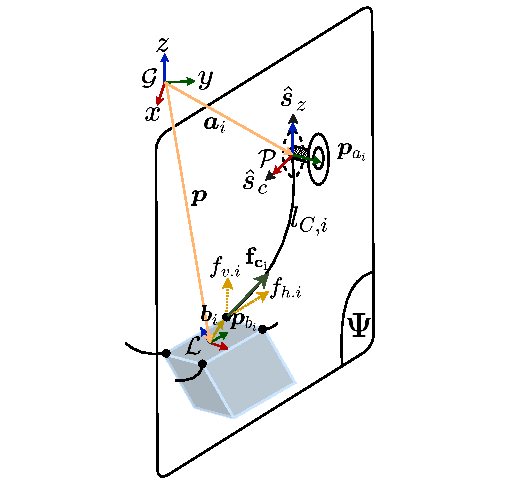
\includegraphics[width=0.6\textwidth]{img/robot_frame.pdf}
	\caption{دیاگرام پنجه ربات متصل به یک کابل  شکم‌دار}
	\label{fig:frame_robot}
\end{figure}

ما تغییر شکل کابل را در یک صفحه عمودی دو بعدی $\Psi$ مدل‌سازی می‌کنیم که پولی $\bm{p}_{a_i}$ و نقطه اتصال $\bm{p}_{b_i}$ در پنجه ربات را در بر می‌گیرد. دستگاه‌مختصات
$\mathcal{P}$
روی این صفحه در نقطه $\bm{p}_{a_i}$ قرار دارد و با بردارهای واحد $\hat{\bm{s}}_z$ که موازی با محور $z$ جهانی است و $\hat{\bm{s}}_c$ که در جهت کابل بر روی صفحه $x_{\mathcal{P}}-y_{\mathcal{P}}$  دستگاه‌مختصات $\mathcal{P}$ قرار دارد، تعریف می‌شود.
به طور خاص،  $\hat{\bm{s}}_c = \frac{\bm{b}_{xy_i} - \bm{a}_{xy_i}}{\|\bm{b}_{xy_i} - \bm{a}_{xy_i}\|}$، که در آن $\bm{b}_{xy_i}$ و $\bm{a}_{xy_i}$ به ترتیب اجزای $x-y$ بردارهای $\bm{b}_{i}$ و $\bm{a}_{i}$ در دستگاه‌مختصات جهانی هستند.

\section{معادلات مدل کابل شکم‌داده} \label{seq:modeling}

معادلات زنجیره‌ای اثر شکم‌یافته کابل غیرقابل ارتجاع با جرم غیر قابل اغماض را همانطور که در~\cite{pott2013cable, irvine1978free} توصیف شده است، به صورت زیر است:

\begin{equation} \label{eq:z(cx)}
	z_i(x_c) = \frac{f_{h,i}}{g_c} \cdot \left( \cosh \left( \frac{g_c}{f_{h,i}} \cdot (x_c + C_{1,i}) \right) - C_{2,i} \right)
\end{equation} 

در این معادله، شکل خمیده کابل با تابع $z_i(x_c)$ تعریف شده است. ثابت‌های زنجیره‌ای، $C_{1,i}$ و $C_{2,i}$ با توجه به شرایط مرزی نقطه انتهایی $z_i(0)=(\bm{p}_{a})_z$ و $z'_i(L_i)=-\frac{f_v}{f_h}$ تعیین می‌شوند، که در آن $z'_i(L_i)$ شیب معادله (\ref{eq:z(cx)}) در \(x_c = L_i = \|(\bm{b})_{xy_i} - (\bm{a})_{xy_i}\|\) است و به صورت زیر دارای ‌حل بسته هستند:

\begin{equation}  \label{eq:C1}
	C_{1,i} = \frac{f_{h,i}}{g_c} \cdot \operatorname{asinh} \left( \frac{-f_{v,i}}{f_{h,i}} \right) - L_i  
\end{equation}

\begin{equation}  \label{eq:C2}
	C_{2,i} = \cosh \left(C_{1,i} \cdot \frac{g_c}{f_{h,i}} \right) - \frac{g_c}{f_{h,i}} \cdot (\bm{p}_a)_z
\end{equation}

همانطور که در شکل~\ref{fig:frame_robot} نشان داده شده است، $f_{h,i}$ و $f_{v,i}$ اجزای افقی و عمودی نیروی کابل $\mathbf{f}_{c_i}$ در دستگاه‌مختصات $\mathcal{P}$ هستند. علاوه بر این، $g_c=g.\rho_c$ است که در آن $g$ و $\rho_c$ به ترتیب شتاب گرانشی و جرم در واحد طول کابل هستند. در نهایت، طول منحنی معادله (\ref{eq:z(cx)}) به عنوان طول واقعی کابل $l_{C,i}$ تعریف می‌شود و به صورت زیر محاسبه می‌شود:

\begin{equation}  \label{eq:lcat}
	\begin{aligned}
		l_{C,i} &= \int_0^{L_i} \sqrt{1 + \left(\frac{dz}{dx}\right)^2} \, dx \\ &= \frac{f_{h,i}}{g_c} \cdot \left( \sinh \left( \frac{g_c}{f_{h,i}} (L_i + C_{1,i}) \right) - \sinh \left( \frac{g_c}{f_{h,i}} \cdot C_{1,i} \right) \right) 
	\end{aligned}
\end{equation}


\section{سینماتیک ربات}   
تحلیل سینماتیکی یک ربات موازی کابلی فروتحریک شامل هر دو معادلات هندسی و حالت ایستای آن است، که به طور معروف به تحلیل سینماتیک-ایستا معروف است~\cite{carricato2013direct}. نیروی پیچشی\footnote{wrench}
 پنجه ربات
 $\mathbf{w}_{ee} \in \mathbb{R}^6$ 
به نیروهای کابل $\mathbf{f}_c \in \mathbb{R}^4 $ از طریق ماتریس ژاکوبی $\bm{J} \in \mathbb{R}^{4\times6}$ مرتبط می‌شود:
\begin{equation} \label{eq:static}
	\mathbf{w}_{ee} = \bm{J}^T \mathbf{f}_{c}  
\end{equation}


در این اینجا، فرض می‌کنیم که $\mathbf{w}_{ee}$ تنها توسط گرانش ایجاد شده است و به صورت زیر محاسبه می‌شود:
\begin{equation} \label{eq:example}
	\mathbf{w}_{ee} = m_{e}g \begin{bmatrix} \hat{\bm{s}}_z \\ \bm{b}_{\text{com}} \times \hat{\bm{s}}_z \end{bmatrix}
\end{equation}

که در آن $m_e$ جرم پنجه ربات و $\bm{b}_{com}$ جابجایی بین مبدا دستگاه‌مختصات $\mathcal{L}$ و مرکز جرم (CoM) انتهای ربات است. 
برای پیوند دادن این معادلات حالت ایستا با مدل زنجیره‌ای در معادله \eqref{eq:lcat}، هر جزء نیروی کابل به عنوان یک جفت افقی و عمودی نمایش داده می‌شود:  
\begin{equation}
	\mathbf{f}_{c_{i}}= \begin{bmatrix} f_{h,i} & f_{v,i} \end{bmatrix} ^T 
\end{equation}

برای هر $\mathbf{f}_{c_{i}}$، ستون $i^{ام}$ مربوطه از ماتریس ژاکوبی $\bm{J}^T$ به صورت زیر بیان می‌شود:
\begin{equation}
	\bm{J}^T_i= \begin{bmatrix} -\hat{\bm{s}}_{c,i} & \hat{\bm{s}}_{z} \\ -\bm{R}\bm{b}_{i} \times \hat{\bm{s}}_{c,i} & \bm{R}\bm{b}_{i} \times \hat{\bm{s}}_{z}  \end{bmatrix}
\end{equation}

که در آن، ماتریس چرخش $\bm{R}$، بردارهای واحد $\hat{\bm{s}}_{c,i}, \hat{\bm{s}}_{z}$، و بردار اتصال پنجه $\bm{b}_i$ در مختصات محلی، در بخش
\ref{subsec:Assm} 
تعریف شده‌اند. توجه داشته باشید که معادلات حالت ایستا در 
\ref{eq:static}
 یک مسئله نامعین\footnote{underdetermined}
است که در آن تعداد معادلات کمتر از تعداد متغیرها است. همانطور که در \cite{allak2022kinematics} پیشنهاد شده است، ما تمام نیروهای کابل را بر اساس یک کابل مرجع بیان می‌کنیم. همانطور که در بخش~\ref{sec:calib_factor} مشاهده خواهد شد، این انتخاب، تعداد حسگرهای نیرو مورد نیاز را به تنها یک عدد کاهش می‌دهد که برای ما نیز از اهمیت بالایی برخودار است. همانطور که در~\cite{borgstrom2009nims, allak2022kinematics} ارائه شده است، با تقسیم ماتریس ژاکوبین و بردار نیرو، می‌توان
 \ref{eq:static} 
 را به صورت زیر نوشت:
\begin{equation} \label{eq:wrench-jac-force}
	\mathbf{w}_{ee} = \begin{bmatrix} \bm{J}^T_{\text{ref}} & \bm{J}^T_{\text{res}} \end{bmatrix} \cdot \begin{bmatrix} \mathbf{f}_{c_{\text{ref}}} \\ \mathbf{f}_{c_{\text{res}}} \end{bmatrix} 
\end{equation} 

که نتیجه می‌دهد:
\begin{equation} \label{eq:jacobian-distribution}
	\mathbf{w}_{ee} = \bm{J}_{\text{ref}}^T \cdot \mathbf{f}_{c_{\text{ref}}} + \bm{J}_{\text{res}}^T \cdot \mathbf{f}_{c_{\text{res}}} 
\end{equation}

که در آن، $\bm{J}^T_{\text{ref}}$ نمایانگر یک زیرماتریس $6\times2$ شامل دو ستون اول $\bm{J}^T$ است که مربوط به نیروی کابل مرجع $\mathbf{f}_{c_{\text{ref}}}$ است. به دنبال آن، $\bm{J}^T_{\text{res}}$ به عنوان زیرماتریس باقی‌مانده $6\times6$ تعریف می‌شود و $\mathbf{f}_{c_{\text{res}}}$ نمایانگر نیروهای کابل باقی‌مانده است. ما می‌توانیم $\mathbf{f}_{c_{\text{res}}}$ را در معادله~\eqref{eq:jacobian-distribution} به صورت زیر بازنویسی کنیم:

\begin{equation} \label{eq:force_base_cable_one}
	\mathbf{f}_{c_{\text{res}}} = (\bm{J}_{\text{res}}^T)^{-1} \left( \mathbf{w}_{ee} - \bm{J}_{\text{ref}}^T \cdot \mathbf{f}_{c_{\text{ref}}} \right)
\end{equation}

با این فرمول‌بندی، تعداد متغیرها از 8 به 2 کاهش می‌یابد، در حالی که معادلات حالت ایستا به‌طور ضمنی در معادله \eqref{eq:static} نهفته می‌شود و نیاز افزودن یک قید جداگانه را حذف می کند~\cite{borgstrom2009nims}.




\section{گراف عامل کالیبراسیون و مکان‌یابی همزمان سینماتیک-ایستا} \label{sec:calib_factor}

در این بخش، با استفاده از روابط استخراج شده در قسمت قبل، و همچنین فرمول‌بندی سینماتیکی تعریف شده در فصل پیشین، رویکردی با یک فرمول‌بندی یکپارچه ایجاد می‌شود. رویکرد ما یک گراف عامل با گره‌های متغیر
$\bm{X}(k) \in SE(3)$، $l^0_i$، $\bm{p}_{a_i} \in \mathbb{R}^3$، $\Delta\mathcal{\bm{R}}(k) \in SO(3)$، و $f^{ref}_{h}(k), \ f^{ref}_{v}(k) \in \mathbb{R}$
تعریف می‌کند. این گره‌ها به ترتیب، نمایانگر مکان‌های پنجه ربات، مقادیر اولیه طول کابل‌ها، مکان‌های نقاط پولی، و تغییرات در جهت‌گیری ربات، و همچنین نیروی کابل مرجع در محورهای افقی و عمودی در حالت‌های ایستا ربات هستند. در ساختار فروتحریک ما، همه ترکیب‌های مکانی و جهت‌گیری قابل اجرا نیستند. در اینجا، $\Delta\mathcal{\bm{R}}(k)$ متغیری است که مقدار اولیه چرخش پنجه ربات را تغییر می‌دهد. علاوه بر این، کابل مرجع به عنوان کابلی که کاربر حسگر نیرو برای مقاصد کالیبراسیون بر روی آن تعبیه شده است، تعیین می‌شود.

\begin{figure} [t]
	\centering
	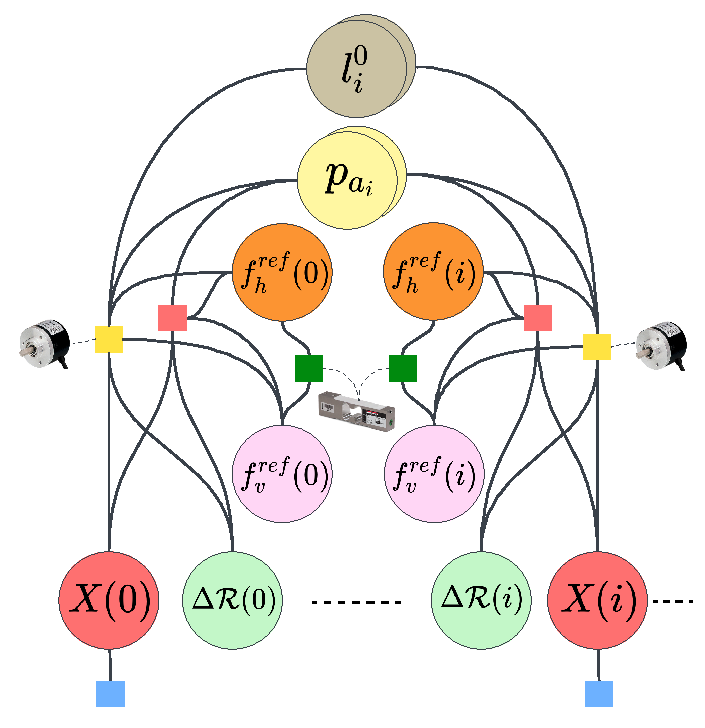
\includegraphics[width=0.55\textwidth]{img/CALIBRATION_GRAPH.pdf}
	\caption{گراف عامل کالیبراسیون و مکان‌یابی همزمان ربات کابلی با کابل‌های شکم‌دار}
	\label{fig:calibration_FG}
\end{figure}

شکل~\ref{fig:calibration_FG} ساختار این گراف عامل در راستای کالیبراسیون خودکار و همچنین مکان‌یابی همزمان برای ساختار تعریف شده را که برای دو نمونه از وضعیت‌های ایستا $0$ و $i$ نمایش داده شده است، نشان می‌دهد. متغیرهای بهینه‌سازی در این گراف با دایره‌های برچسب‌خورده با نام‌های پارامتر‌ها در رنگ‌های مختلف نمایان شده‌اند.
علاوه بر این، عامل‌ها با مربع‌های رنگی به تصویر کشیده شده‌اند، که عامل انکودر و یا همان طول کابل شکم‌دار به رنگ زرد، عامل مکان اتصال کابل به پولی به رنگ قرمز، عامل اندازه‌گیری نیرو به رنگ سبز، و عامل پیشین مکان به رنگ آبی است. هر عامل بر اساس معادلات سینماتیک و مدل ریاضی تعریف شده برای کابل توصیف‌شده در بخش
\ref{seq:modeling}
 فرمول‌بندی شده و به شرح زیر تعریف می‌شوند:

\subsection{عامل طول کابل شکم‌دار}
این عامل رابطه‌ای بین اندازه‌گیری‌های انکودر و طول واقعی کابل از معادله
\ref{eq:lcat}
 ایجاد می‌کند. این قید اندازه‌گیری برای کابل $i^{ام}$ به صورت زیر فرمول‌بندی می‌شود:
\begin{equation}
	f(z^{enc}_{i}, \bm{\zeta})[k] = l_{C,i}[k] + l^0_i - z^{enc}_{i}[k]
\end{equation}

که در آن $l_{C,i}$ نمایانگر طول واقعی کابل در اثر شکم‌دهی از نیروی وزن آن  به‌طوریکه در معادله~\ref{eq:lcat} تعریف شده است، می‌باشد. همچنین $l^0_i$ نشان‌دهنده مقدار طول اولیه کابل است، و $z^{enc}_{i}$ نمایانگر اندازه‌گیری نسبی انکودر مربوط به کابل $i^{ام}$ است. علاوه بر این، $k$ بیان‌کننده شاخص نمونه داده‌های زمانی است.

\subsection{عامل مکان اتصال کابل به پولی}
این عامل تضمین می‌کند که ارتفاع محاسبه‌شده نقطه اتصال کابل روی پنجه ربات، که از مکان پنجه ربات استنتاج شده، با ارتفاع کابل شکم‌دار پیش‌بینی‌شده از پولی مربوطه مطابقت داشته باشد. تابع خطا برای پولی $i^{ام}$ به صورت زیر بیان می‌شود:
\begin{equation}
	f(\bm{\zeta})[k] = (p_{b,i})_z [k] - z_i(L_i)[k]
\end{equation}
که در آن، $(p_{b,i})_z$ به ارتفاع نقطه اتصال کابل $i^{ام}$ در مختصات جهانی اشاره دارد، و $z_i(L_i)$ نمایانگر شکل شکم‌دهی کابل در $L_i$ به‌طوریکه در معادله~\ref{eq:z(cx)} توصیف شده است.

\subsection{عامل اندازه‌گیری نیرو}
این عامل نرم نیروی افقی و عمودی را به‌گونه‌ای محدود می‌کند که نزدیک به اندازه‌گیری نیرو از حسگر تعبیه‌شده روی کابل مرجع، در نزدیکی پنجه ربات باشد. توجه داشته باشید که این محدودیت تنها برای کابل مرجع با یک تابع هزینه به صورت زیر مورد نیاز است:
\begin{equation}
	f(f^{m}, \bm{\zeta})[k] = \| [f^{ref}_{h}[k]~~f^{ref}_{v}[k]]^T \| - f^{m}[k]
\end{equation}
در اینجا، $f^{ref}_{h}$ و $f^{ref}_{v}$ به ترتیب نمایانگر نیروهای مرجع کابل در جهت‌های افقی و عمودی هستند، $\|.\|$ نشان‌دهنده نرم اقلیدسی است، و $f^{m}$ مقدار  نیروی کابل مرجع است که توسط حسگر نیرو اندازه‌گیری شده است.

\subsection{عامل پیشین مکان}
عوامل انکودر و اندازه‌گیری نیرو با گره‌های متغیر مکان $\bm{X}(k)$ مرتبط هستند که نمایانگر وضعیت‌های ایستا ربات در فرآیند کالیبراسیون به‌طوریکه توسط یک سیستم محلی‌سازی مبتنی بر بینایی اندازه‌گیری شده است. 
هر مکان به حالات تعادلی مربوط می‌شود که در آن ربات از طریق چهار کابل خود ثابت است. نمونه‌هایی از وضعیت‌های ایستا در شکل~\ref{fig:calibration_FG} با نشانگرهای $0$ و $i$ برچسب‌گذاری شده‌اند. این عامل پیشین  مکان نیز برای تعریف صفر ربات مورد استفاده قرار می‌گیرد.



\section{نتایج شبیه سازی} \label{sec:results}
این بخش به منظور اعتبارسنجی مدل و روش کالیبراسیون پیشنهادی از طریق شبیه‌سازی اجزای محدود\footnote{\lr{Finite Element (FE)}}
 سیستم ارائه شده است. ابتدا اعتبار فرمول‌بندی‌های سینماتیک-ایستا بررسی می‌شود و سپس نتایج کالیبراسیون برای دو ربات کابلی کوچک مقیاس و بزرگ مقیاس نشان داده می‌شود. برای شبیه‌سازی‌های اجزای محدود از نرم‌افزار RecurDyn~\cite{functionbay} استفاده خواهیم کرد، مدل گراف عامل خود را با استفاده از کتابخانه GTSAM~\cite{dellaert2012factor} پیاده‌سازی می کنیم و همچنین از SymForce~\cite{Martiros-RSS-22} برای استخراج مشتق عامل‌ها و ژاکوبین‌های مربوطه استفاده می‌کنیم.


نرم‌افزار \lr{RecurDyn} یک نرم‌افزار مهندسی به کمک رایانه\footnote{\lr{Computer-Aided Engineering (CAE)}}
است که توسط شرکت \lr{FunctionBay} توسعه داده شده و در شبیه‌سازی دینامیک چندجسمی\footnote{\lr{Multibody Dynamics (MBD)}}
 سیستم‌های مکانیکی که از اجسام سخت یا انعطاف‌پذیر متصل به هم تشکیل شده‌اند، تخصص دارد. این نرم‌افزار به مهندسان اجازه می‌دهد حرکت و تعاملات این سیستم‌ها را شبیه‌سازی و تحلیل کنند تا رفتار آن‌ها در شرایط واقعی را پیش‌بینی کنند. \lr{RecurDyn} با ابزارهای تحلیل اجزا محدود\footnote{\lr{Finite Element Analysis (FEA)}}
  برای تحلیل اجسام انعطاف‌پذیر که تحت تنش ها تغییر شکل می‌دهند، یکپارچه شده و از هم‌زمان‌سازی با سایر ابزارهای \lr{CAE} و سیستم‌های کنترلی پشتیبانی می‌کند. همچنین این نرم‌افزار امکان سفارشی‌سازی از طریق برنامه‌نویسی را فراهم می‌کند. \lr{RecurDyn} به طور گسترده در صنایع مختلفی مانند خودروسازی، رباتیک، هوافضا و ماشین‌آلات صنعتی برای بهینه‌سازی عملکرد و طراحی سیستم‌ها استفاده می‌شود. ما نیز از این نرم‌افزار برای شبیه‌سازی اجزا محدود کابل استفاده می‌کنیم.

\subsection{صحت‌سنجی مدل}
برای صحت‌سنجی دقت مدل سینماتیک-ایستا، همان‌طور که در بخش 
\ref{seq:modeling}
توضیح داده شده است، گراف عامل سینماتیک-ایستا توسعه داده شده را با استفاده از عامل‌های پیشین بر روی متغیرهای استخراج شده از شبیه‌ساز مقید می‌کنیم. دو سناریوی ربات کابلی معلق کوچک و بزرگ مقیاس برای صحت‌سنجی این مدل انجام شده است. هدف از طراحی این دو سناریوی مجزا، بررسی دقت الگوریتم برای طیف وسیعی از پیاده‌سازی‌ها می‌باشد. شکل~\ref{fig:recurdyn_small} و شکل~\ref{fig:recurdyn_large} این سناریوهای ربات‌ها را در محیط شبیه‌ساز RecurDyn نشان می‌دهند. هر دو ربات چهار کابل را به چهار گوشه بالای یک جعبه مستطیلی  متصل کرده‌اند. همچنین ابعاد ربات که از فواصل بین پولی ها که در شکل مشخص شده‌اند به دست آمده، $(12.5, 4.5, 28.5)$ متر برای ربات کوچک و $(240, 220, 50)$ متر برای ربات بزرگ‌تر در نظر گرفته شده است. همان‌طور که در جدول~\ref{tab:Model_verification} ذکر شده است، جرم پنجه برای ربات بزرگ $34 \text{ Kg}$ و برای ربات کوچک $4.4 \text{ Kg}$ تنظیم شده است. چگالی طول کابل‌ها برای ربات کوچک $10.2 \text{ g/m}$ و برای ربات بزرگ‌تر $72.4 \text{ g/m}$ است، که به نسبت جرم پنجه ربات به کابل $4.14$ برای ربات کوچک و $0.62$ برای ربات بزرگ‌تر نتیجه می‌دهد. همان‌طور که در~\cite{pott2013cable} پیشنهاد شده است، این شرایط نشان‌دهنده تأثیر قابل توجه شکم‌دهی برای ربات بزرگ‌تر است.

\begin{figure} [t]
	\centering
	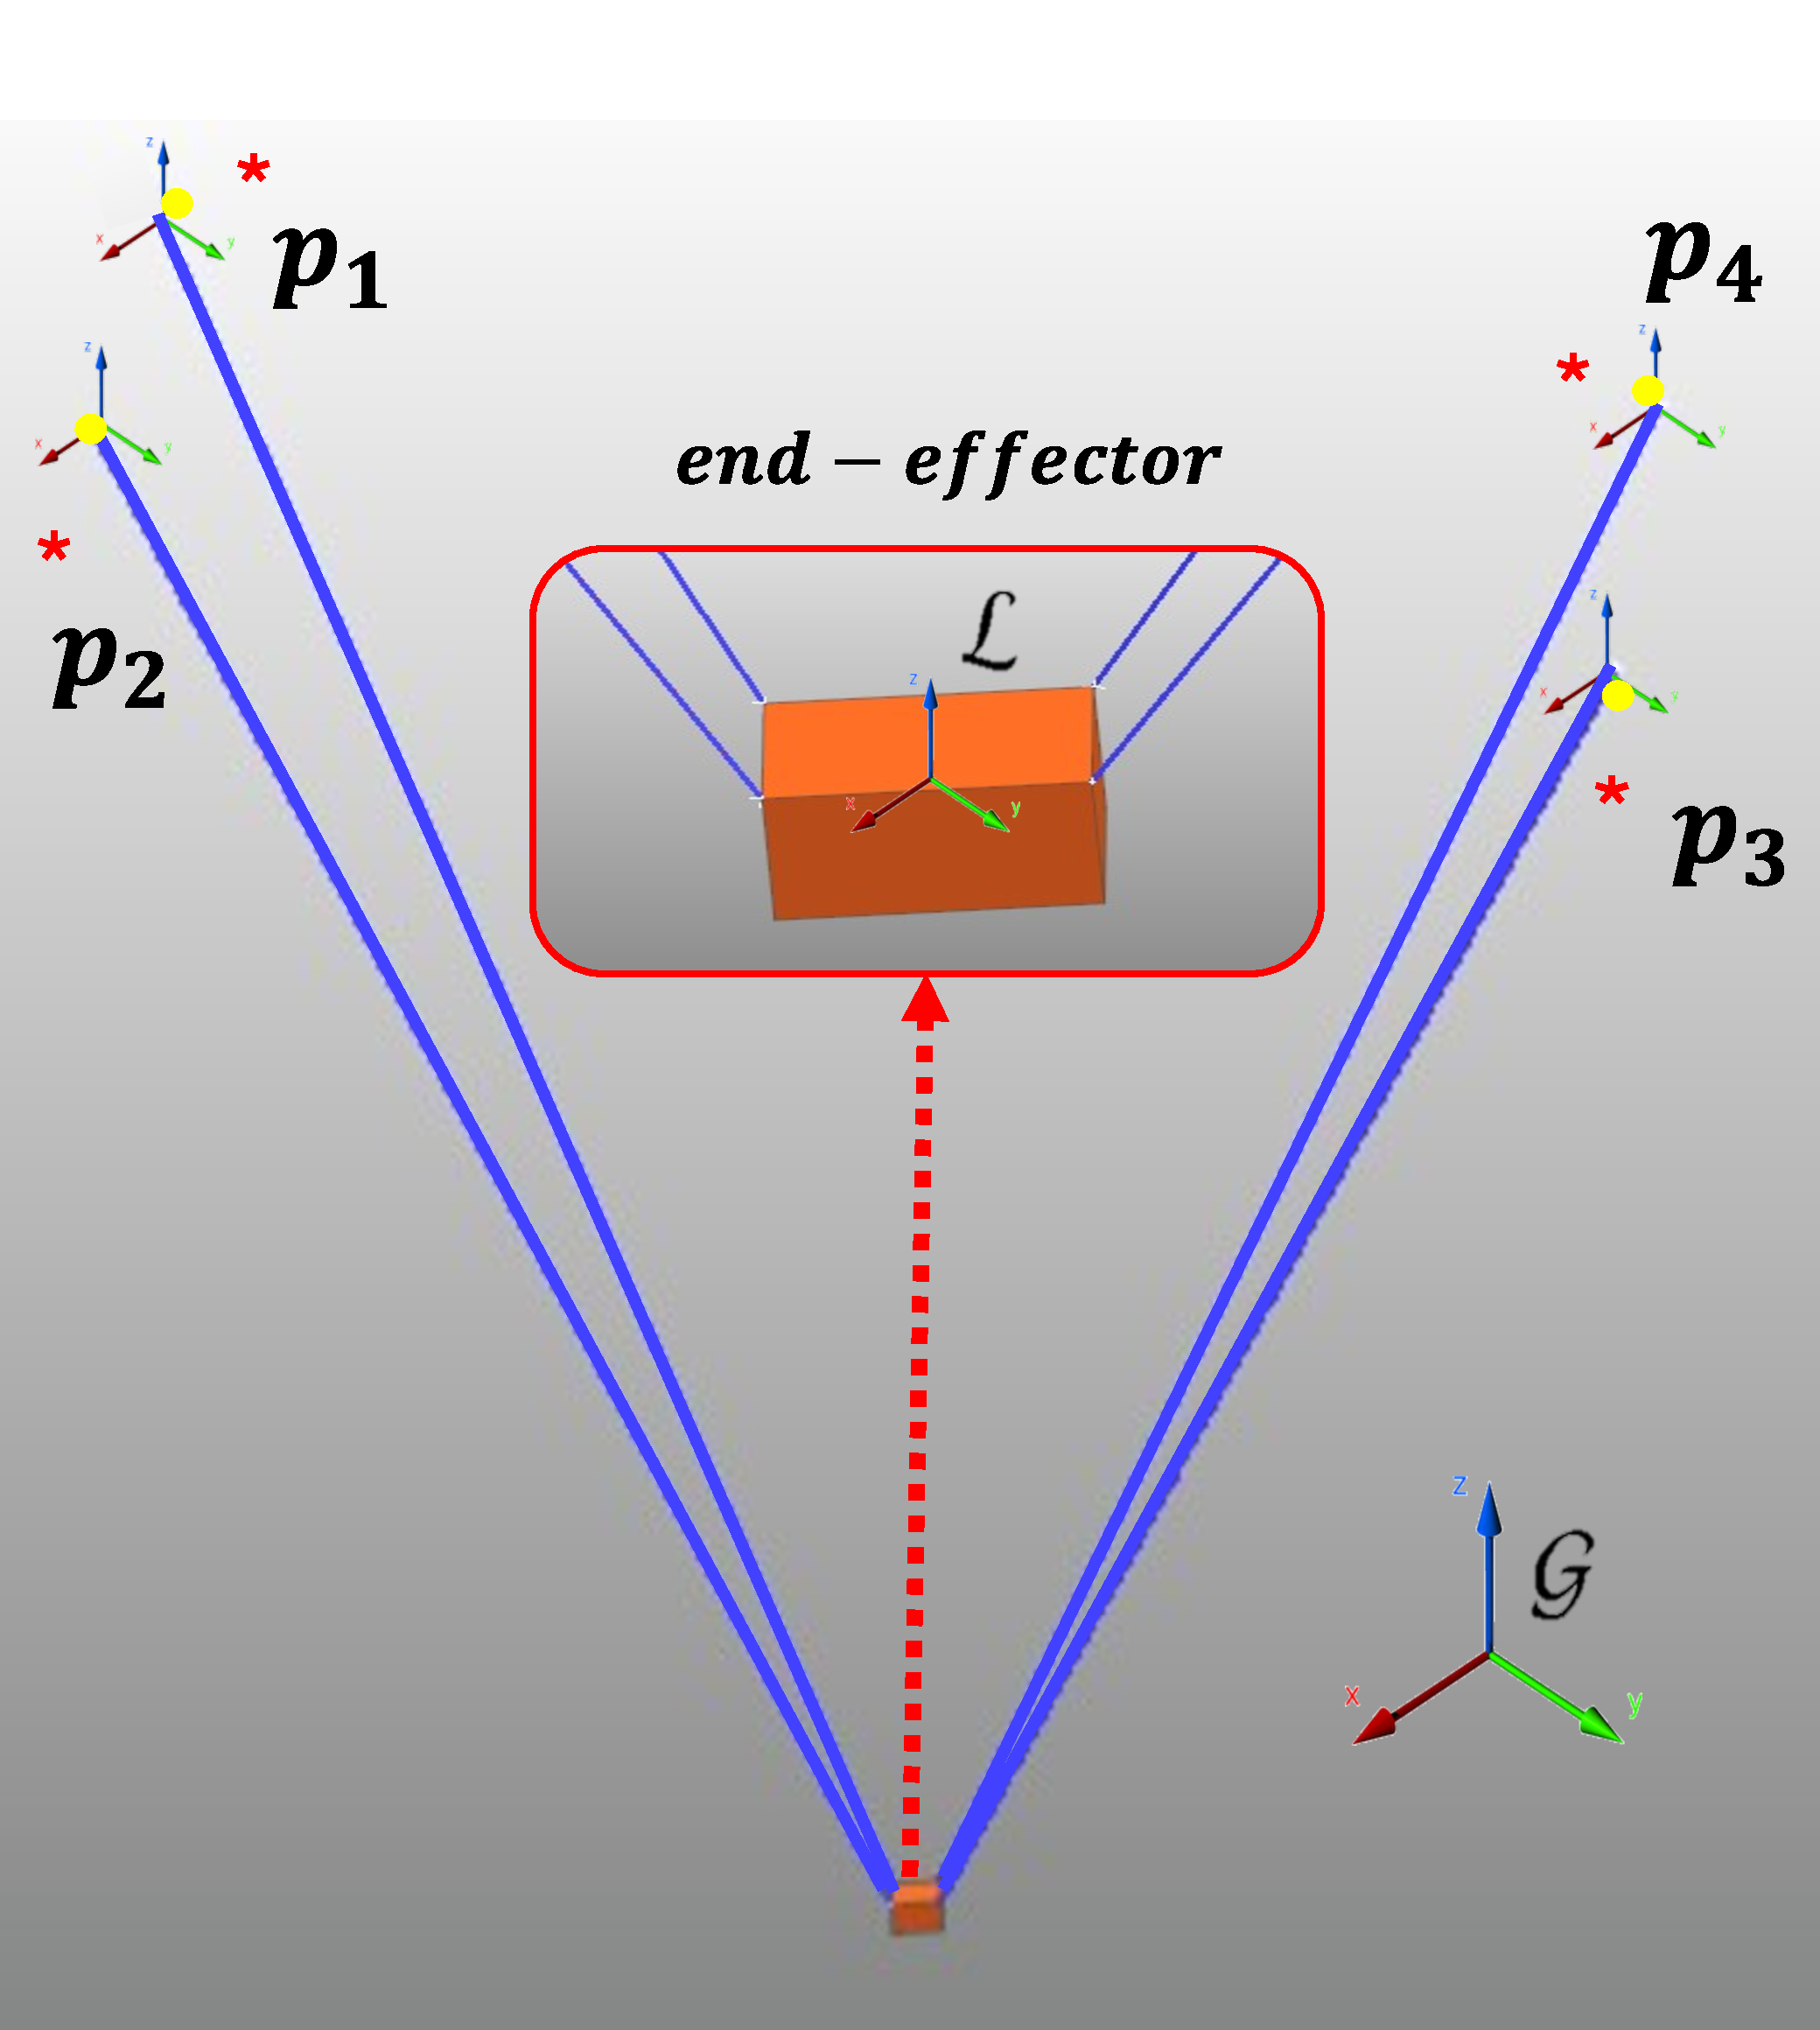
\includegraphics[width=0.45\textwidth]{img/E2_small.pdf}
	\caption{سناریوی ربات کوچک‌مقیاس در محیط شبیه‌ساز RecurDyn}
	\label{fig:recurdyn_small}
\end{figure}

\begin{figure} [b]
	\centering
	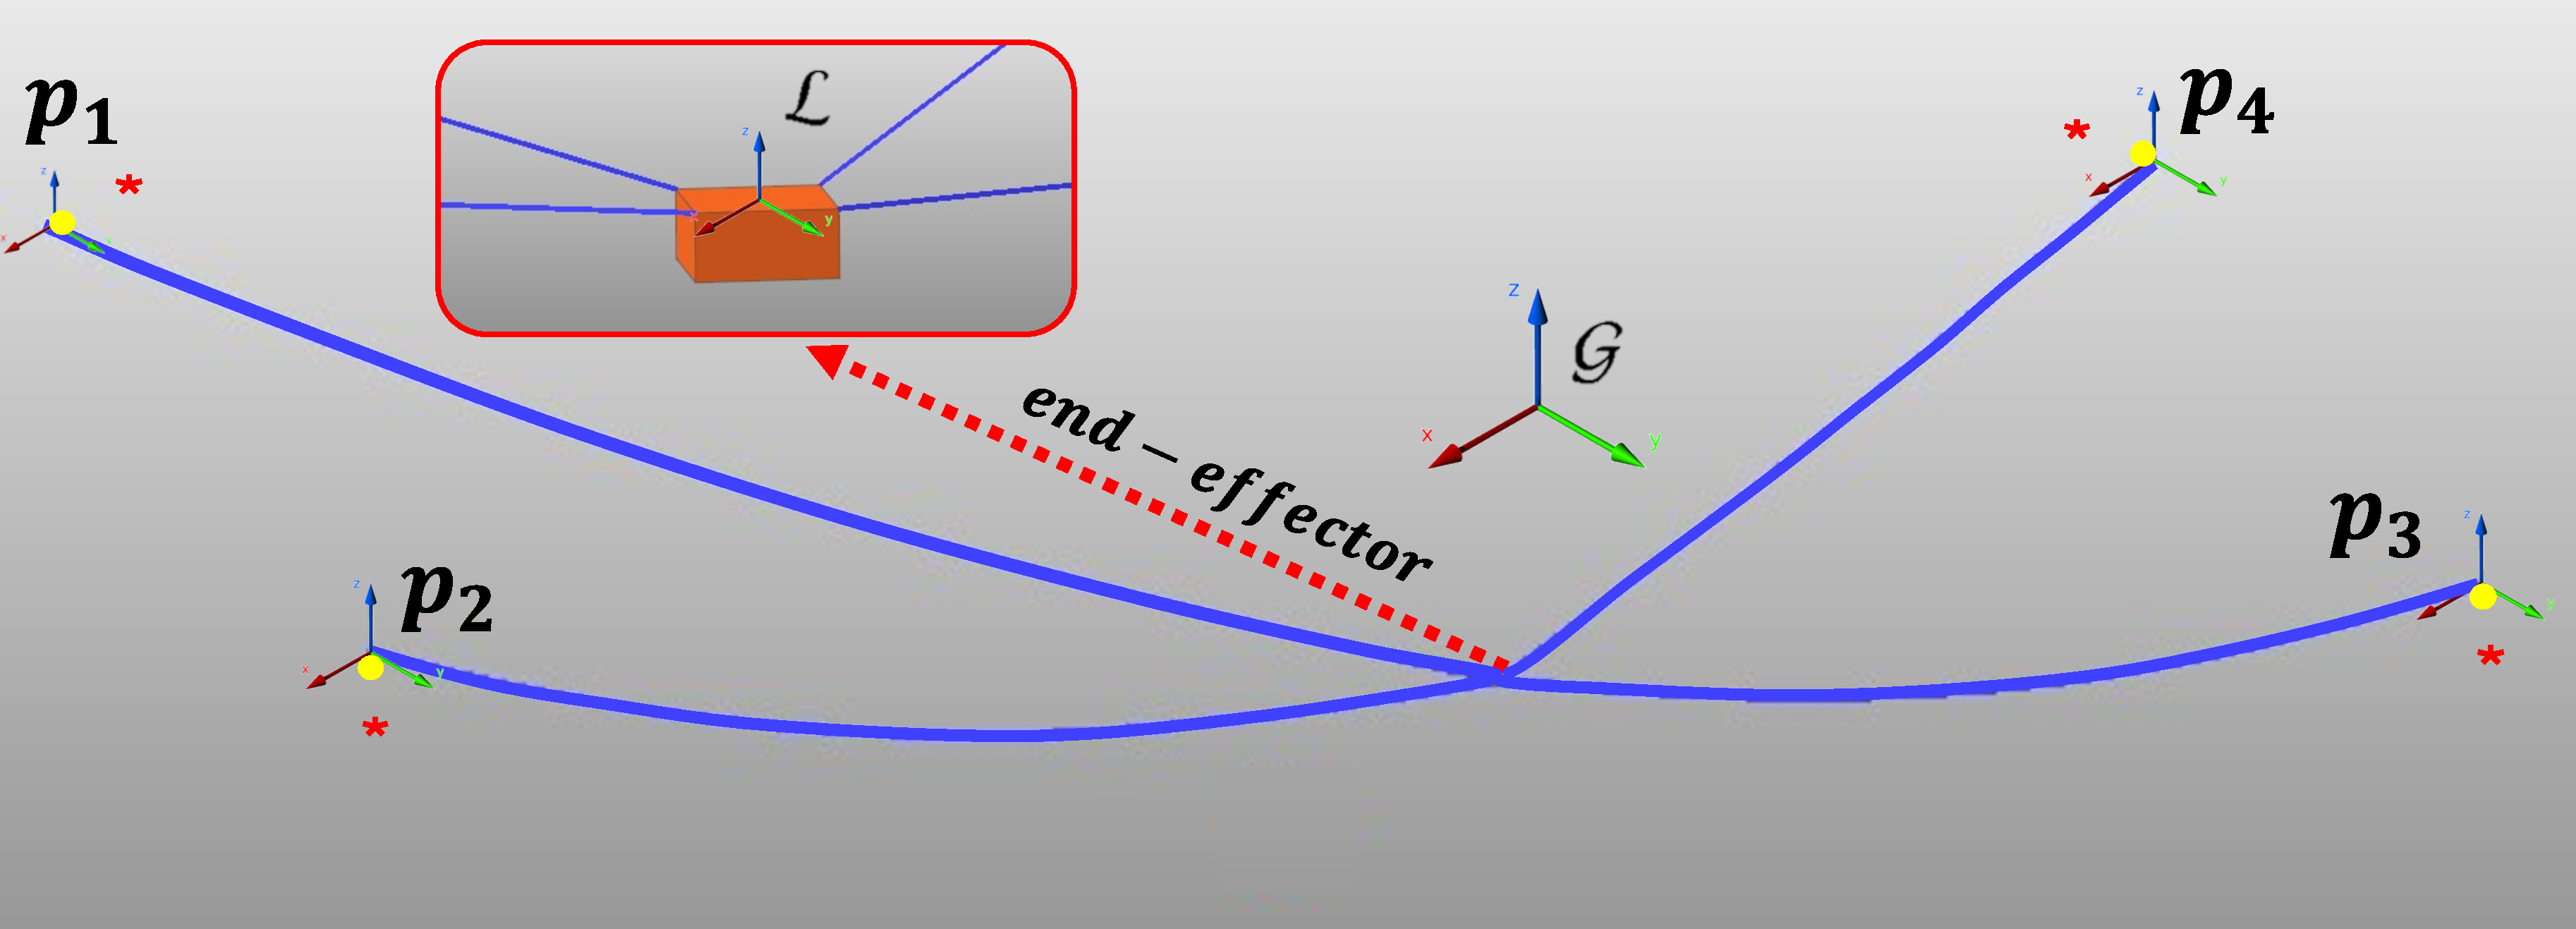
\includegraphics[width=0.8\textwidth]{img/E1_large.pdf}
	\caption{سناریوی ربات بزرگ‌مقیاس در محیط شبیه‌ساز RecurDyn}
	\label{fig:recurdyn_large}
\end{figure}

دو ردیف اول جدول~\ref{tab:Model_verification} درصد خطاهای میانگین در طول کابل پیش‌بینی شده (MPE-L) و همچنین این خطا برای نیرو (MPE-F) محاسبه شده در 5 مکان ایستای تصادفی را ارائه می‌دهد. این مقادیر نشان‌دهنده‌ی تطابق نزدیک بین نیروی کابل و مقادیر طول کابل شکم‌دار محاسبه شده از مدل ریاضی ارائه شده و مقادیر مربوطه از شبیه‌ساز می‌باشد. به طور خاص، برای ربات بزرگ مقیاس، این خطاهای MPE-L و MPE-F به ترتیب برابر با
 $0.0089\%$ 
 و 
 $0.9154\%$ 
 ارزیابی شده است، که بسیار کوچک‌تر از دامنه‌های طول کابل و نیرو‌های ایجادشده برای هر کابل، مطابق مقادیر گزارش شده در جدول، می‌باشد. همان‌طور که به طور شهودی انتظار می‌رود، این تطابق برای ربات کابلی کوچک‌تر دقیق‌تر است. مقادیر مربوط به طول کابل و نیروهای پیش‌بینی شده در ستون سوم این جدول نشان‌دهنده این موضوع می‌باشند.

\begin{table}
	\centering
	\caption{صحت‌سنجی مدل}
	\label{tab:Model_verification}
	\renewcommand{\arraystretch}{1.45} % Increase row spacing
	\footnotesize
	\begin{tabular}{c|c|c}
		\toprule
		\rowcolor{gray!10}
		\hline
		\text{سناریو} & \text{‌بزرگ‌مقیاس} & \text{‌کوچک‌مقیاس} \\
		\midrule
		(\%) MPE-L  & $8.8947\times10^{-3}$ & $7.3595\times10^{-3}$ \\
		\hline
		(\%) MPE-F  & $0.9154$ & $0.9046$ \\
		\hline
		$[l_{\min}, l_{\max}](m)$ & $[134.7, 200.7]$ & $[10.8, 25.9]$ \\
		\hline
		$[f_{\min}, f_{\max}](N)$ & $[489.1, 954.3]$ & $[12.4, 26.2]$ \\
		\hline
		اندازه ربات ($\text{m}^3$) & $240\times220\times50 $ & $12.5\times 4.5 \times 28.5$ \\
		\hline
		جرم پنجه ربات ($\text{Kg}$) & $34.0$ & $4.4$ \\
		\hline
		\multirow{2}{*}{مشخصات کابل} & \multirow{2}{*}{\begin{tabular}[c]{@{}c@{}} $\rho = 1.44~~(\text{g}/\text{cm}^2)$ \\ 
				$\text{شعاع} = 4.0~~(\text{mm})$ \end{tabular}} & \multirow{2}{*}{\begin{tabular}[c]{@{}c@{}} $\rho = 1.44~~(\text{g}/\text{cm}^2)$ \\ $\text{شعاع} = 1.5~~(\text{mm})$  \end{tabular}} \\
		& & \\
		\bottomrule
	\end{tabular}
\end{table}


\subsection{نتایج نهایی کالیبراسیون با گراف عامل توسعه‌ داده‌شده}
در قسمت، روش کالیبراسیون را که در بخش 
\ref{sec:calib_factor}
توضیح داده شده است، پیاده‌سازی می‌کنیم و اهمیت مدل‌سازی شکم‌دهی کابل را از طریق نتایج شبیه‌سازی نشان می‌دهیم. علاوه بر این، به طور خلاصه به مسئله مقداردهی اولیه کالیبراسیون پرداخته و یک راه‌حل احتمالی را همچون فصل قبل، پیشنهاد می‌کنیم.

هدف ما در فرآیند کالیبراسیون سینماتیکی، تعیین مکان‌های نقطه‌های پولی و طول اولیه کابل‌ها با استفاده از اندازه‌گیری‌های مجموعه‌ای از مکان‌های پنجه ربات، اندازه‌گیری‌های طول نسبی کابل و تنها مقادیر کشش کابل مرجع در نقطه اتصال پنجه است. طبق آزمایشات و نتایجی که از طیف وسیعی از داده‌ها استخراج شده است، توزیع نمونه‌ها بایستی به طور جامع فضای‌کاری ربات را پوشش دهد. تحلیل و توسعه مسیر مناسب برای جمع‌آوری کمترین تعداد داده در جهت انجام فرآیند کالیبراسیون موفق، به موضوع تحقیق آینده برای تکمیل این کار محول می‌شود.

ما داده‌های حسگر شبیه‌سازی شده خود را از نرم‌افزار RecurDyn دریافت کردیم و تغییرات نویز گاوسی میانگین صفر را برای وارد کردن نویز پیش‌بینی‌شده حسگر معرفی کردیم. به طور خاص، ما انحراف استاندارد\footnote{\lr{Standard Deviation {STD}}} 
$10mm$ 
برای طول کابل، $5N$ برای حسگر نیرو در ربات بزرگ‌مقیاس و $1N$ برای حسگر ربات کوچک‌مقیاس اعمال کردیم. مکان‌های پنجه ربات با $\Delta \mathbf{T} = \exp(\hat{\boldsymbol{\xi}})$ که در آن $\hat{\boldsymbol{\xi}} \in \mathfrak{se}(3)$ عنصر جبر لی\footnote{\lr{Lie algebra}}
 متناظر با بردار پیچش\footnote{\lr{screw vector}}
  $\boldsymbol{\xi} \in \mathbb{R}^6$
 است، دچار تغییر شده‌اند. این بردارهای پیچش تغییرات، از توزیع گاوسی میانگین صفر $\boldsymbol{\xi}\sim\mathcal{N}(\mathbf{0}, \boldsymbol{\Sigma})$ با ماتریس کوواریانس $\boldsymbol{\Sigma}$ با انحراف $0.005$ متر در درجات انتقالی و $0.01$ رادیان در درجات آزادی چرخشی نمونه‌برداری شده‌اند.
برای مقداردهی اولیه گراف عامل، مکان‌های نقطه‌های پولی از شبیه‌ساز به عنوان داده‌های مرجع را با دامنه $1$ متر برای ربات کوچک و $10$ متر برای  ربات بزرگ دچار تغییر کردیم. علاوه بر این، این تغییرات برای مقادیر اولیه طول کابل‌ها، $10$ متر و $80$ متر برای ربات کوچک و بزرگ، به ترتیب، تنظیم شد. ما تخمین اولیه برای نیروی کابل مرجع در محور عمودی را به عنوان:
\begin{equation}  \label{eq:fv_0}
	f^{{ref}}_{v_0} = \frac{m_eg}{4}
\end{equation}
  در نظر گرفتیم و برای محور افقی نیز به صورت زیر:
\begin{equation}  \label{eq:fh_0}
	f^{ref}_{h_0}=\frac{f^{{ref}}_{v_0}}{\tan(\alpha)} 
\end{equation}
که در آن $\alpha$ به صورت زیر تعریف می‌شود:
\begin{equation}  \label{eq:alpha}
	\alpha = \arccos\left(\frac{\hat{\bm{s}}_{c_{ref}}^T \cdot [\bm{p}_{b_{\text{ref}}} - \bm{p}_{a_{\text{ref}}}]}{\| \bm{p}_{b_{\text{ref}}} - \bm{p}_{a_{\text{ref}}} \|}\right)
\end{equation}
در این تعریف، $\hat{\bm{s}}_{c_{ref}}$ بردار واحدی است که در بخش \ref{seq:modeling} تعریف شده است و از تخمین‌های اولیه مکان پولی استفاده می‌کند. این نقاط باید به پولی‌های مربوط به کابل مرجع متقابل مربوط ‌شوند.

نتایج کالیبراسیون برای مکان‌های پولی و طول اولیه کابل در جدول~\ref{tab:calibration_results_sag} ارائه شده است. این نتایج مربوط به سناریوهای نشان داده شده در شکل~\ref{fig:recurdyn_small} و شکل~\ref{fig:recurdyn_large} است، که در آن مکان‌های اولیه پولی با ستاره‌های قرمز و مکان‌های بهبودیافته پولی‌ با دایره‌های زرد برای هر دو مورد نشان داده شده است.
در این جدول، سه سناریوی مختلف کالیبراسیون برای ربات بزرگ‌مقیاس با تعداد مختلف نقاط نمونه‌برداری شده (یا همان تعداد داده‌ها برای کالیبراسیون) برای فرآیند بهینه‌سازی گزارش شده است. همان‌طور که انتظار می‌رود، دقت کالیبراسیون با افزایش تعداد داده‌های نمونه‌برداری بهبود می‌یابد. بنابراین جدول~\ref{tab:calibration_results_sag} نتایج دقیق‌تری را با 35 نمونه داده برای ربات بزرگ و 8 نمونه برای ربات کوچک ارائه می‌دهد. ما معتقدیم که برای ربات بزرگ‌تر، پارامترهای مربوط به شکم‌دهی کابل تأثیر عمیق‌تری بر دقت کالیبراسیون دارند. این موضوع به نوبه خود تعداد مؤثر پارامترهای مدل را افزایش می‌دهد و نیاز به نقاط نمونه‌برداری بیشتری برای شناسایی مناسب دارد.

\begin{table}
	\centering
	\caption{نتایج میانگین خطای مطلق کالیبراسیون با استفاده از گراف عامل توسعه‌ داده‌شده}
	\label{tab:calibration_results_sag}
	\renewcommand{\arraystretch}{1.3} % Increase row spacing
	\footnotesize
	\begin{tabular}{c|c|c|c|c}
		\toprule
		\rowcolor{gray!10}
		\hline
		\text{میانگین خطا(متر)} & \text{مقیاس‌بزرگ (9 داده)} & \text{مقیاس‌بزرگ (18 داده)} & \text{مقیاس‌بزرگ (35 داده)} & \text{مقیاس‌کوچک (8 داده)} \\
		\midrule
		$\text{پولی(متر)}$ &  $0.387$ &  $0.226$  &   $0.191$  &   $0.149$ \\
		\hline
		$\text{طول اولیه کابل(متر)}$ &  $0.380$  &  $0.217$  &   $0.173$  &   $0.115$ \\
		\bottomrule
	\end{tabular}
\end{table}

حل شدن مسئله بهینه‌سازی کالیبراسیون در کنار زنجیره‌ای از پارامتر‌های مکان‌یابی که به مدل کابل‌، داده‌های حسگریِ پنجه ربات و وضعیت مفصل‌های ربات مقید شده است، حلی دقیق‌تر از مسئله را برای ما فراهم می‌کند. حرکت ربات در فضا می تواند منجر به ایجاد وضعیت‌های ایستا شود که در هر کدام از این وضعیت‌ها، قیدهای مربوط به سینماتیک به زنجیره‌ مکان‌یابی متصل می‌شود. وجود تعدادی محدود از این قیود می تواند نقش مهمی در بهبود مکان ربات پس از مدتی حرکت در فضا را ایجاد کند و از خطاهای جمع‌شونده که از نویز حسگر‌ها القا می‌شود، جلوگیری شود. عملکرد این قید همچون نشانگرهایی که در SLAM مورد استفاده قرار می‌گیرند، در اینجا نیز بسیار کارآمد هستند. از آنجایی که هدف ما در این فصل توسعه پایه و اساس الگوریتم مد نظر و مقیدسازی آن با قیدهای پیچیده‌تر بود، از ایجاد پیچیدگی بیشتر در قسمت مکان‌یابی اجتناب گردید. افزودن قیود مکان‌یابی و توسعه بیشتر الگوریتم در این راستا، کار دشواری نخواهد بود. 

موضوع دیگری که در فرمول‌بندی تعریف شده مورد توجه قرار دارد، صادق بودن معادلات طول شکم‌دار کابل در حالت ایستای ربات است. به همین دلیل، داده‌هایی که برای کالیبراسیون مورد استفاده قرار داده‌ شد، داده‌‌های حالت‌های ایستای ربات بودند. البته، حل مسئله در فضایی جامع‌تر، و نه محدود به داد‌های ایستا، نیازمند تغییر فرمول‌بندی به معادلات در فضای اجزای محدود می باشد. این توسعه و تحقیق به کارهای آینده سپرده شده‌است.


\section{بحث و گفت‌وگو} \label{sec:discussion}

\subsection{اهمیت در نظر گرفتن اثر شکم‌دهی کابل}
برای بررسی اهمیت در نظر گرفتن اثر شکم‌دهی کابل، فرآیند کالیبراسیون را برای ربات بزرگ‌تر با استفاده از یک گراف عامل ساده‌سازی شده که در آن مدل کابل بی‌وزن منعطف به کار رفته بود و در فصل پیشین معرفی شد، انجام دادیم. به عبارتی دیگر، در این آزمایش، گراف عامل مربوط به شکم‌دهی کابل از گراف توسعه‌یافته در این فصل حذف شد. 

نتایج نشان داد که این ساده‌سازی منجر به افزایش قابل توجه خطای میانگین مطلق از $0.19$ به $2.34$ متر شد. این افزایش چشمگیر در خطا، بیانگر اهمیت حیاتی در نظر گرفتن اثر شکم‌دهی کابل در مدل‌سازی و کالیبراسیون است. در واقع، شکم‌دهی کابل نه تنها به دلیل تاثیر مستقیم بر طول واقعی کابل و نیروهای اعمالی بلکه به دلیل تاثیر غیرمستقیم آن بر دقت نهایی مکان‌یابی نیز بسیار مهم است.

این تفاوت قابل توجه در کیفیت کالیبراسیون نشان می‌دهد که نادیده گرفتن چنین پارامترهای فیزیکی مهم می‌تواند به کاهش قابل توجه دقت مدل منجر شود و بر عملکرد کلی سیستم تأثیر منفی بگذارد. علاوه بر این، در سیستم‌های بزرگ‌مقیاس که تغییرات کوچک در مدل می‌تواند تأثیرات بزرگی داشته باشد، اهمیت این نکته دوچندان می‌شود. این نتایج تأکید می‌کنند که برای دستیابی به دقت بالا در فرآیندهای کالیبراسیون و مکان‌یابی، مدل‌سازی دقیق و جامع از پارامترهای فیزیکی کابل‌ها، از جمله شکم‌دهی، ضروری است. این نکته نه تنها برای ربات‌های کابلی بلکه برای هر سیستم مکانیکی دیگری که به دقت بالا نیاز دارد، قابل تعمیم است.


\subsection{نکات مربوط به روش مقداردهی اولیه}
همان‌طور که در~\cite{khorrambakht2023graph} ذکر شده است، یکی از نگرانی‌های اصلی در حل مسئله بهینه‌سازی کالیبراسیون غیرمقعر و غیرخطی، مقداردهی اولیه صحیح آن است. اگر مقادیر اولیه به اندازه کافی نزدیک به راه‌حل جهانی مسئله نباشند، نتیجه ممکن است به شدت منحرف شود یا بهینه‌ساز حتی ممکن است واگرا شود. چارچوب ارائه شده در~\cite{khorrambakht2023graph} که در فصل پیشین نیز مورد استفاده قرار گرفت، تلاش می‌کند تا این مسئله مقداردهی اولیه را با استفاده از خروجی تقریبی یک الگوریتم بهینه‌سازی جهانی مونت کارلو حل کند. با این حال،~\cite{khorrambakht2023graph} مدل کابل منعطف بدون اثرات شکم‌دهی را فرض می‌کند. ما معتقدیم که این الگوریتم به طور مستقیم می‌تواند برای مقداردهی اولیه مسئله کالیبراسیون توسعه یافته ارائه شده در این فصل به کار رود. همان‌طور که قبلاً ذکر شد، دقت کالیبراسیون ربات کابل بزرگ با مدل کابل ساده شده $2.34$ متر بود. این مقدار به طور قابل توجهی کوچکتر از تغییرات ما در طول آزمایشات کالیبراسیون ($10$ متر) است. این نشان می‌دهد که ما می‌توانیم با خیال راحت الگوریتم بهینه‌سازی خود را با خروجی‌های الگوریتم مشابهی که در~\cite{khorrambakht2023graph} ارائه شده است، مقداردهی اولیه کنیم. تأیید این فرضیه برای موارد خاص ارائه شده در این فصل به دلیل محدودیت‌های شبیه‌ساز مورد استفاده برای تولید تصاویر/داده‌های حسگر LiDAR مورد نیاز برای اجرای این الگوریتم امکان‌پذیر نبود. بررسی این ایده با استفاده از شبیه‌سازهای واقع‌گرایانه موضوع تحقیق آینده‌ی ما است.



\section{نتیجه‌گیری}
این فصل با هدف توسعه گراف عامل معرفی شده در فصل قبل و بررسی میزان دشواری افزودن قید به یک مسئله فرمول‌بندی شده در فضای گراف، تدوین گردید. همان‌طور که مشاهده شد، مقید‌سازی این مسئله، حتی با وجود قیدهای بسیار پیچیده، در این فضای گراف پایه به‌طور نسبی ساده است. این فصل توانست شرایطی از کالیبراسیون و مکان‌یابی یک ربات واقعی را شبیه‌سازی کرده و نتایج ارزشمندی را برای اولین بار در فضای ربات‌های کابلی مقیاس بزرگ با استفاده از روش‌های بهینه‌سازی گراف‌پایه ارائه دهد.

نتایج حاصل نشان داد که مدل‌سازی دقیق اثر شکم‌دهی کابل‌ها در ربات‌های کابلی، تأثیر قابل‌توجهی در بهبود دقت کالیبراسیون و مکان‌یابی دارد. با استفاده از گراف عامل پیشنهادی، امکان بررسی و مدل‌سازی دقیق‌تر شرایط واقعی کابل‌های شکم‌دار فراهم شده است که در نهایت منجر به کاهش خطاهای ناشی از فرضیات ساده‌سازی‌شده در مدل‌های پیشین شد. این نتایج تأکید می‌کند که توجه به جزئیات دینامیکی و فیزیکی کابل‌ها، اهمیت ویژه‌ای در بهبود دقت فرآیندهای کالیبراسیون و مکان‌یابی ربات‌ها دارد.

فرمول‌بندی توسعه داده‌شده در این فصل، با بهره‌گیری از معادلات سینماتیک-ایستا و استفاده از گراف عامل، توانسته است مکان‌های پولی و طول‌های اولیه کابل‌ها را با دقت بالایی تخمین بزند. نتایج شبیه‌سازی‌ها نشان داد که دقت کالیبراسیون به تعداد داده‌های نمونه‌برداری شده بستگی دارد و با افزایش این داده‌ها، نتایج دقیق‌تری به دست می‌آید. این رویکرد نه تنها عملکرد ربات‌های کابلی را در شرایط مختلف بهبود بخشید، بلکه اهمیت توجه به اثرات پیچیده‌تر دینامیکی مانند شکم‌دهی کابل در فرآیندهای کالیبراسیون را برجسته کرد.

در نهایت، تحقیقات انجام‌شده در این فصل، راه را برای مطالعات بیشتر در زمینه بهبود الگوریتم‌های کالیبراسیون ربات‌ها با در نظر گرفتن اثرات دینامیکی هموار کرده است. این نتایج می‌توانند به‌طور بالقوه به پیشرفت‌های قابل‌توجهی در صنایع مختلف از جمله ربات‌های خودران، حمل‌ونقل و فضانوردی منجر شوند. با این حال، علیرغم ایجاد یک شالوده محکم برای پیش‌برد اهداف تحقیقاتی آینده، برخی از مسائل مانند ادغام داده‌های حسگری اضافی با دقت بالا برای اهداف همجوشی حسگرها و بهبود روش‌های مقداردهی اولیه با استفاده از راه‌حل‌های کارآمد معرفی شده در این حوزه، نیازمند بررسی‌های عمیق‌تر در تحقیقات آینده هستند. بهبود و توسعه این جنبه‌ها می‌تواند نتایج حاصل از این تحقیق را به سطوح جدیدی از دقت و کاربرد برساند و در نهایت، زمینه‌ساز نوآوری‌های آینده در حوزه ربات‌های کابلی شود.



		% فصل پنجم: نتایج
% !TeX root=../main.tex


\chapter{نتیجه‌گیری و پیشنهادات برای آینده}
%\thispagestyle{empty} 
\section{نتیجه‌گیری}

در این پایان‌نامه، در فصل اول و دوم، ابتدا مروری بر مسائل بهینه‌سازی در ادبیات ربات‌ها صورت گرفت. مشاهده شد که این مسائل با توجه به اهداف کاربردی ربات‌ها، می‌توانند دارای ماهیت‌های متفاوت، اما ضروری باشند. با نگاهی اجمالی به ادبیات موضوع، مشخص شد که این مسائل بهینه‌سازی می‌توانند در راستای فرمول‌بندی یک مسئله کالیبراسیون دینامیکی یا سینماتیکی، مکان‌یابی، ردیابی، نقشه‌برداری، یا ترکیبی از این موارد باشند.

در فصل سوم، با آغاز فرمول‌بندی‌های مرسوم برای ایجاد یک مسئله کالیبراسیون و مکان‌یابی همزمان، به نقطه ضعف‌هایی برخوردیم که نه تنها ایجاد فرمول‌بندی مورد نظر را دشوار می‌کردند، بلکه در حل چنین مسائل پیچیده‌ای به صورت زمان واقعی با تعداد بسیار زیادی داده، ناتوان بودند. از سوی دیگر، انعطاف‌پذیری الگوریتم برای افزودن قیود جدید به مسئله بدون تغییر در فرمول‌بندی، برای ما بسیار حائز اهمیت بود، زیرا مقیدسازی سینماتیکی می‌تواند دقت مکان‌یابی را به‌طور قابل توجهی افزایش دهد. با در نظر گرفتن تمامی این نکات و استفاده از آخرین روش‌ها و حل‌کننده‌های موجود در رباتیک، الگوریتم‌های گراف مبنا را به‌عنوان راه‌حلی مناسب در فضای حل احتمالاتی این مسائل انتخاب کردیم. بدین ترتیب، از مکان‌یابی یک ربات شروع کردیم و با توسعه گراف عامل مناسب، مسائل کالیبراسیون در سطوح مختلف و همچنین قیود ضروری، به گراف توسعه‌یافته متصل گردید. در انتهای این فصل، گراف عامل جامع پیشنهادی خود برای حل مسئله کالیبراسیون و مکان‌یابی ربات‌ها، با تمرکز بر رفع مشکلات روش‌های مرسوم، معرفی شد.

در ادامه، برای صحت‌سنجی روش پیشنهادی، از میان ربات‌های موجود، ربات کابلی آسان‌نصب انتخاب گردید. علت این انتخاب، اهمیت انجام همزمان فرآیند کالیبراسیون و مکان‌یابی این ربات‌ها در کوتاه‌ترین زمان ممکن برای ایجاد مفهوم یک ربات آسان‌نصب بود. بدین ترتیب، در فصل چهارم، با استفاده از ربات کابلی صلب توسعه‌یافته در مجموعه آزمایشگاهی ارس، الگوریتم پیشنهادی مورد بررسی قرار گرفت. در این پیاده‌سازی، اهمیت قیود سینماتیکی در بهبود نتایج مکان‌یابی یکی از چالش‌های مورد بررسی بود. علاوه بر این، کالیبراسیون سینماتیکی به‌صورت خودکار برای ربات، در حالی که مکان‌یابی در حال انجام بود، صورت گرفت و نتایج قابل قبولی از نظر سرعت الگوریتم و توانایی آن در برآورد اهداف ما به‌دست آمد.

در نهایت، برای محک‌زدن روش پیشنهادی و همچنین نمایش انعطاف‌پذیری آن، گامی جدید در ادبیات ربات‌های کابلی برداشته شد. فصل پنجم، به حل همان مسئله ربات‌های کابلی که در فصل چهارم مطرح شده بود، می‌پردازد. اما آنچه به‌عنوان نوآوری این فصل و نقطه پایانی کار معرفی گردید، افزودن یکی از پیچیده‌ترین قیود دینامیکی به مسئله ربات‌های کابلی برای مدل‌سازی واقعی‌تر کابل و گسترش روش موردنظر برای همه ربات‌های کابلی بدون نگرانی از ابعاد ربات و مسئله خم‌شدگی کابل‌ها بود. نتایج کالیبراسیون برای دو دسته ربات کوچک‌مقیاس و بزرگ‌مقیاس در یک شبیه‌ساز اجزای محدود مورد بررسی قرار گرفت. بررسی  و مقایسه این نتایج با به‌کارگیری روش‌های فصل چهارم، علاوه بر بهبود قابل توجه، نقطه عطفی برای تحقیقات در زمینه ترکیب سنسورها و کاربرد آن‌ها در مسائل ربات‌های کابلی بود.

\section{پیشنهادات برای آینده}

در مسیر انجام این پایان‌نامه، موانع متعددی به وجود آمد که گذر از آنها افق‌های جدیدی را برای نویسنده نمایان کرد و چشم‌اندازهای تازه‌ای را در جهت ایجاد نقطه‌ای مفید در این حوزه مشخص ساخت. علاوه بر نظراتی که در راستای توسعه الگوریتم ایجاد شده است، نظرات متعددی نیز در بخش پیاده‌سازی به وجود آمدند، چرا که پیچیدگی حل چنین مسائلی در ربات‌های کابلی باعث شده است تحقیقات مفید و کارآمدی در این زمینه کمتر صورت گیرد. برخی از این پیشنهادات در گروه در حال پیش‌برد می‌باشند و برخی به عنوان کار‌های بعدی مدنظر خواهند بود. 

\begin{itemize}
	
\item {\textbf{ایجاد گراف‌های عامل با استفاده از کتابخانه :SymForce} 
در این پایان‌نامه، از کتابخانه GTSAM برای ایجاد گراف‌های عامل استفاده شده است. یکی از چالش‌برانگیزترین بخش‌های حل مسئله، محاسبه ژاکوبین مدل بود. نرم‌افزارهای متعددی مانند Maple و MATLAB، و همچنین کتابخانه‌های مختلفی همچون SymPy در پایتون و AutoDiff در C++ مورد استفاده قرار گرفتند. با این حال، حجم بسیار بالای معادلات دینامیکی کابل‌ها، مانع از به دست آوردن پاسخ در این بسترها شد. 

در نهایت، با استفاده از کتابخانه SymForce که مشتق‌گیری‌ها را با روش‌های مشتق‌گیری خودکار
\footnote{\lr{Automatic Differentiation}} 
 انجام می‌دهد، موفق شدیم تمامی مشتق‌های مورد نیاز را در زمانی کمتر از ۳۰ ثانیه محاسبه کنیم. 
پیشنهاد ما در این بخش، نه تنها استفاده از این کتابخانه برای به دست آوردن ژاکوبین‌های مورد نیاز است، بلکه پیشنهاد می‌شود که گراف‌های عامل توسعه‌یافته نیز با استفاده از روش‌هایی که به تازگی توسط این کتابخانه ارائه‌شده، ایجاد شوند. ما معتقدیم که این رویکرد می‌تواند فرآیند ایجاد گراف‌های عامل را به طور قابل توجهی ساده‌تر کند.}



\item \textbf{پیاده‌سازی ماژول بهینه‌ساز سینماتیک-استاتیک ربات کابلی توسعه‌یافته در راستای بهبود دقت ردیابی:} 
در زمینه ربات‌های کابلی، ادغام داده‌های سینماتیکی می‌تواند به طور قابل توجهی در بهبود نتایج ردیابی کمک کند. در فصل چهارم این پایان‌نامه، بخشی از نتایج این موضوع را اثبات کردند. وقتی به حوزه ربات‌های مقیاس‌بزرگ وارد می‌شویم، در نظر گرفتن دینامیک کابل، همانطور که در فصل پنجم مشاهده شد، بسیار حائز اهمیت می‌شود. 

در همین راستا، مقاله \cite{allak2022kinematics} در سال‌های اخیر سعی در توسعه روشی برای ردیابی ربات‌های کابلی با در نظر گرفتن جرم کابل، به صورت منابع باز داشته است. حل‌کننده‌ی پیشنهادی آنها، CERES، علیرغم توانایی بالای خود در حل مسئله، عیوب روش‌های مرسوم را دارد. 

در قسمتی از کارهای انجام شده توسط ما، بررسی حل‌کننده مورد استفاده توسط این مقاله برای ربات‌های مقیاس‌بزرگ بوده است. در حالی که نتایج حل بهینه‌سازی توسط گراف عامل پیشنهادی ما و حل پیشنهادی این مقاله برای ربات‌های کوچک‌مقیاس مشابه بود، افزایش ابعاد ربات باعث واگرایی در الگوریتم ارائه شده در مقاله می‌شود. این در حالی است که گراف عامل پیشنهادی به خوبی برای ربات‌های مقیاس‌بزرگ نتیجه را دنبال می‌کند.

علاوه بر این، در این مقاله برای ادغام نتایج بهینه‌سازی سینماتیکی با حسگر‌های مختلف از فیلتر کالمن استفاده شده است که خود نیاز به ایجاد ساختاری جدا و اتصال این دو، و همچنین ادغام مناسب داده‌های حسگر اینرسی-بینایی دارد. روش پیشنهادی ما استفاده از ماژول طراحی‌شده است. استفاده از این ماژول نه‌تنها منجر به همگرایی در ربات‌های با ابعاد بزرگ‌تر می‌شود، بلکه ادغام حسگرها برای قسمت ردیابی بسیار راحت‌تر و منجر به حل دقیق‌تری می‌شود. افزون بر این موارد، گره‌هایی که به تازگی برای ادغام حسگرهای اینرسی در این حوزه معرفی شده‌اند، بسیار ارزشمند خواهند بود. لازم به ذکر است که این ماژول بااستفاده از معادلات ارائه شده در فصل پنجم ایجاد شده است که یکی از ویژگی‌های مهم آن حذف نیاز به حسگر نیروِ، با استفاده از قید‌های سینماتیک وارون می‌باشد. 

\item \textbf{کالیبراسیون حسگر UWB با استفاده از گراف عامل پیشنهادی:} 
حسگرهای UWB به دلیل ویژگی‌های خاص خود در کاربردهای مختلف تعیین مکان در حوزه‌های نقشه‌برداری و رباتیک مورد استفاده قرار می‌گیرند. این حسگرها را می‌توان در دو سطح کالیبراسیون بررسی کرد.

سطح اول، حذف بایاس‌های اولیه است. این نوع کالیبراسیون، مشابه روش ارائه‌شده در فصل چهارم است. به عبارتی، اگر در گراف عامل فصل چهارم حسگرهای نیرو حذف شوند و مقادیر اندازه‌گیری حسگرهای UWB جایگزین مقادیر اندازه‌گیری انکودر شوند، نه‌تنها قادر به تعیین این آفست‌ها خواهیم بود، بلکه مکان اتصال انکرها می‌تواند به عنوان مکان پولی‌ها در نظر گرفته شده و یک مسئله بهینه‌سازی ایجاد شود.

سطح دوم کالیبراسیون این حسگرها، در نظر گرفتن این بایاس اولیه به عنوان پارامتری متغیر با زمان است. به عبارتی، گراف عامل فصل چهارم را در حالتی ایجاد کنیم که بایاس حسگر UWB همانند متغیر سینماتیکی مجموعه، همانطور که در انتهای فصل سوم بررسی شد، در حال تغییر باشد. بدین ترتیب، کالیبراسیون با دقت بالایی به‌صورت زمان واقعی انجام می‌شود. انجام این سطح کالیبراسیون نسبت به سطح اول، حذف بایاس‌های متغیر با زمان سیستم می‌باشد که در سطح اول از آنها صرف‌نظر می‌شود. این پیشنهاد در مرحله اجرا توسط اعضای تیم آزمایشگاهی ارس می‌باشد.


\item \textbf{پیاده‌سازی الگوریتم گراف پیشنهادی برای ربات‌های واقعی مقیاس بزرگ:} 
تمامی موارد بررسی‌شده در فصل چهارم بر روی ربات کابلی واقعی توسعه‌یافته در تیم آزمایشگاهی ارس پیاده‌سازی شده‌اند. در فصل پنجم، این پیاده‌سازی واقعی نیازمند یک ربات در ابعاد ورزشگاه بزرگ است که با توجه به امکانات فعلی، پیاده‌سازی واقعی برای ما مقدور نبوده است. همچنین هیچ‌گونه دیتاست‌ای از چنین ربات با ابعاد بزرگ در اینترنت نیز در دسترس نیست. به همین دلیل، از داده‌های شبیه‌سازی نرم‌افزار RecurDyn استفاده کردیم. البته که نتایج خود، نویزهای شدیدی که برای نزدیک شدن به یک پیاده سازی واقعی در نظر گرفته ایم. پیشنهاد ما پیاده‌سازی مجدد روش‌های پیشنهادی در فصل پنجم بر روی یک ربات واقعی است. تمامی کدهای مورد نیاز برای این پیاده‌سازی به‌صورت منابع باز در Github قرار داده شده است.

\item \textbf{ایجاد شبیه‌ساز مناسب ربات کابلی با استفاده از توابع آماده شده:} 
ما برای توسعه یک ربات کابلی با ابعاد بزرگ نرم‌افزار های متعددی مورد بررسی قرار دادیم که از انجام این شبیه‌سازی باز ماندند. بهترین نرم‌افزاری که با محاسبات بسیار طولانی و زمان‌بر ما را به جواب رساندند، نرم‌افزار RecurDyn بوده است. پیشنهاد ما توسعه یک محیط گرافیکی مناسب برای معرفی یک نرم‌افزار شبیه‌ساز کابل با در نظر گرفتم جرم کابل، با استفاده از توابع سینماتیکی و مکان‌یابی معرفی شده در فصل‌های اخیر می‌باشد. چنین نرم‌افزاری که دارای سرعت بالا باشد طبق آخرین تحقیقات ما توسعه نیافته است.

\item \textbf{ایجاد یک شبیه‌ساز مناسب ربات کابلی با استفاده از توابع آماده‌شده:}
ما برای توسعه یک ربات کابلی با ابعاد بزرگ، نرم‌افزارهای متعددی را مورد بررسی قرار دادیم، اما اغلب آن‌ها نتوانستند شبیه‌سازی مورد نظر ما را انجام دهند. بهترین نرم‌افزاری که با وجود محاسبات طولانی و زمان‌بر، توانست به نتایج مطلوب برسد، نرم‌افزار RecurDyn بود. پیشنهاد ما توسعه یک محیط گرافیکی مناسب برای معرفی یک نرم‌افزار شبیه‌ساز کابل با در نظر گرفتن جرم کابل، و استفاده از توابع سینماتیکی و مکان‌یابی معرفی‌شده در فصل‌های اخیر است. تاکنون، طبق آخرین تحقیقات ما، چنین نرم‌افزاری که دارای سرعت بالا باشد، توسعه نیافته است.

\item \textbf{توسعه فرمول‌بندی ریاضی بیان شده به ریاضیات اجزای محدود به جای مدل‌های استاتیک معرفی‌شده:}
مدل توسعه‌یافته برای کابل‌ها در این پایان‌نامه، مبتنی بر مدل‌های ریاضی است که در حالت استاتیک ربات و ثابت بودن کابل‌ها ایجاد شده‌اند. ادغام این الگوریتم با بیان ریاضی فعلی و قیدهای دینامیکی در ربات‌های کابلی به‌صورت مستقیم امکان‌پذیر نخواهد بود. یکی از پیشنهادهای مناسب در امتداد این کار، تغییر فرمول‌بندی به مدلی جامع‌تر است که قابلیت ادغام با تمامی قیدهای دینامیکی ربات را داشته باشد. این تغییر می‌تواند به استفاده مؤثرتر از ریاضیات اجزای محدود به جای مدل‌های استاتیک منجر شود که راه‌حلی برای ما خواهد بود.

\item \textbf{بررسی مسیر مناسب برای جمع‌آوری داده کافی برای کالیبراسیون دقیق:}
همان‌طور که در نتایج مشاهده شد، برای ربات کابلی با مقیاس بزرگ، افزایش تعداد داده‌ها منجر به نتیجه‌ای بهتر در کالیبراسیون خواهد شد، چرا که پارامترهای غیرخطی بسیاری در مدل درگیر هستند. مسیری که در آزمایشات ما طی شد، یک مسیر تصادفی بود که شامل قسمت‌های مختلفی از فضای کاری ربات می‌شد. پیشنهاد ما بررسی این موضوع برای یافتن مسیری بهینه، و نه تصادفی، جهت تسریع فرآیند کالیبراسیون است. این موضوع می‌تواند به بهبود دقت و کاهش زمان کالیبراسیون کمک شایانی کند.


\item \textbf{ترکیب حسگر‌ها و ماژول‌های آماده مختلف:}
در نهایت، این پایان‌نامه بستری کامل برای حل مسائل کالیبراسیون و مکان‌یابی ربات‌ها ایجاد کرده است. بررسی تحقیقات تکمیلی جهت بهبود نتایج و استفاده از ماژول‌های معرفی شده در حوزه رباتیک و به‌ویژه شاخه SLAM می‌تواند نقطه عطف تازه‌ای بین روش‌های موجود در ربات‌های کابلی و روش‌های موجود در دیگر ربات‌ها مانند ربات‌های خودران باشد. این نکته به‌عنوان پیشنهاد ما مطرح می‌شود زیرا اولین هدف ما، حرکت به سمت الگوریتمی منعطف بوده است تا تحقیقات در این حوزه‌ها بیشتر به هم متصل شوند.


\end{itemize}
		% فصل شش: بحث و نتیجه‌گیری

% مراجع
% اگر از استیل‌های natbib استفاده می‌کنید باید دو خط را در فایل commands.tex تغییر دهید.
\pagestyle{empty}
{
\small
\onehalfspacing
\bibliographystyle{unsrt-fa} % or plainnat-fa for author-date
\bibliography{./tex/MyReferences}
}

%\pagestyle{fancy}

\appendix
% فصلهای پس از این قسمت به عنوان ضمیمه خواهند آمد.

% دستورات لازم برای تبدیل «فصل آ» به «پیوست آ» در فهرست مطالب
\addtocontents{toc}{
\protect\renewcommand\protect\cftchappresnum{\appendixname~}%
\protect\setlength{\cftchapnumwidth}{\mylenapp}}
    
% دستورات لازم برای شماره‌گذاری صفحات پیوست‌ها بشکل آ-۱ (فعلا با glossaries سازگار نیست)
%\let\Chapter\chapter
%\pretocmd{\chapter}{
%\clearpage
%\pagenumbering{arabic}
%\renewcommand*{\thepage}{\rl{\thechapter-\arabic{page}}}}{}{}
%%%%%%%%%%%%%%%%%%%%%%%%%%%%%%%%%%%%%        

\chapter{گراف عامل در رباتیک} \label{sec:appendix1}

\section{تئوری}

در زمینه رباتیک و SLAM، گراف‌های عامل ابزارهای قدرتمندی برای تخمین بهینه حالت هستند. در این پایان‌نامه، ما نیز از این ابزار به عنوان یک چارچوب مؤثر برای شناسایی پارامترها استفاده می‌کنیم. در این بخش، مروری کوتاه بر نظریه‌ها و اصول پشت این روش ارائه می‌دهیم. در اینجا، مفاهیم را در زمینه تخمین حالت توضیح می‌دهیم.

در رباتیک، ترکیب حسگرها می‌تواند به عنوان یک مسئله استنتاج بیزی به شرح زیر فرمول‌بندی شود:
\begin{equation} \label{eq:MAP}
	X^{MAP} = \arg\max_X p(X|Z) = \arg\max_X \frac{p(Z|X)p(X)}{p(Z)}
\end{equation}

که در آن \(Z\) و \(X\) به ترتیب نشان‌دهنده مشاهدات توسط حسگرها و حالت‌های سیستم هستند. تخمین بیشینه پسین
\footnote{\lr{Maximum A Posteriori (MAP)}}
 از حالت‌ها، \(X^{MAP}\)، که نتیجه ترکیب است، از طریق بیشینه‌سازی توزیع پسین \(p(X|Z)\) با استفاده از الگوریتم درست‌نمایی بیشینه
\footnote{\lr{Maximum Likelihood (ML)}}
بدست می‌آید. در این فرمول‌بندی، \(p(Z|X)\) تابع احتمال است که مدل مشاهده حسگرها را نشان می‌دهد، در حالی که \(P(X)\) دانش پیشین از حالت سیستم است. همانطور که در ادامه خواهیم دید، در یک سیستم دینامیکی، این دانش پیشین با استفاده از تابع تحول حالت مدل‌سازی می‌شود.

اگر فرض کنیم \(X\) یک فرایند تصادفی مارکوفی است و \(p(Z|X)\) و \(p(X)\) توزیع‌های نرمال باشند، الگوریتم $ML$ به یک مسئله کمینه مربعات
\footnote{\lr{Least Square (LS)}}
 منجر می‌شود.  حال سیستم غیرخطی زیر را در نظر می‌گیریم:
\begin{equation}
	X_{k+1} = f(X_k, u_k) + w(k), \text{~~~~~~~~~~~~~~~~} z_k = h(X_k) + v(k)
\end{equation}


که در آن \(f(X)\) و \(h(X)\) به ترتیب مدل‌های سیستم و اندازه‌گیری هستند. علاوه بر این، \(v(k)\) و \(w(k)\) نویز گاوسی افزایشی با کوواریانس‌های \(R\) و \(Q\) هستند که به ترتیب نویز اندازه‌گیری و عدم قطعیت مدل را نمایش می‌دهند. بردار \(u_k\) ورودی اختیاری به سیستم است و \(X\) حالت‌های سیستم است. تابع احتمال ممکن است به صورت زیر نوشته شود:
\begin{equation} \label{eq:Gauess_Dis_h}
	p(z|x) = \mathcal{N}(z; h(x), R) = \frac{1}{\sqrt{2\pi R}} \exp \left\{ -\frac{1}{2} \| h(x) - z \|_R^2 \right\}
\end{equation}

این شهود وجود دارد که وقتی حالت \(X\) است، انتظار داریم مشاهده \(h(x)\) باشد. بنابراین،
اندازه‌گیری‌های \(z\) که بسیار متفاوت از \(h(x)\) هستند، کمتر احتمال دارد که رخ دهند. علاوه بر این،
هر چه حسگر دارای نویز کمتری باشد، می‌توانیم با اطمینان بیشتری در مورد این انتظار صحبت کنیم. این
شهود در معادله فوق با استفاده از یک تابع توزیع گاوسی مدل‌سازی شده است که
مرکز آن در \(h(x)\) و واریانس \(R\) است.

از طرف دیگر، توزیع پیشین \(p(X)\) انتظار ما از حالت جدید را بدون داشتن اطلاعاتی به‌جز تخمین قبلی نشان می‌دهد. این دانش از
درک ما از سیستم دینامیکی ناشی می‌شود، که در این حالت، با تابع \(f(X)\)
در معادله
\ref{eq:Gauess_Dis_F}
 نمایش داده می‌شود. بنابراین، مشابه تابع احتمال، توزیع پیشین نیز ممکن است
با استفاده از چگالی گاوسی زیر مدل‌سازی شود:
\begin{equation} \label{eq:Gauess_Dis_F}
	p(x_{k+1}|x_k, u_k) = \frac{1}{\sqrt{2\pi Q}} \exp \left\{ -\frac{1}{2} \| f(x_k, u_k) - x_{k+1} \|_Q^2 \right\}
\end{equation}

اکنون، با توجه به این چگالی‌ها، الگوریتم ML به مسئله LS غیرخطی زیر
منجر می‌شود:
\begin{equation}
	\hat{X}_k = \min_X \left( \sum_{i=0}^k \left(\| f(x_i, u_i) - x_{i+1} \|_Q^2 + \| h(x_i) - z_i \|_R^2 \right) \right)
\end{equation}

\begin{figure} [!t]
	\centering
	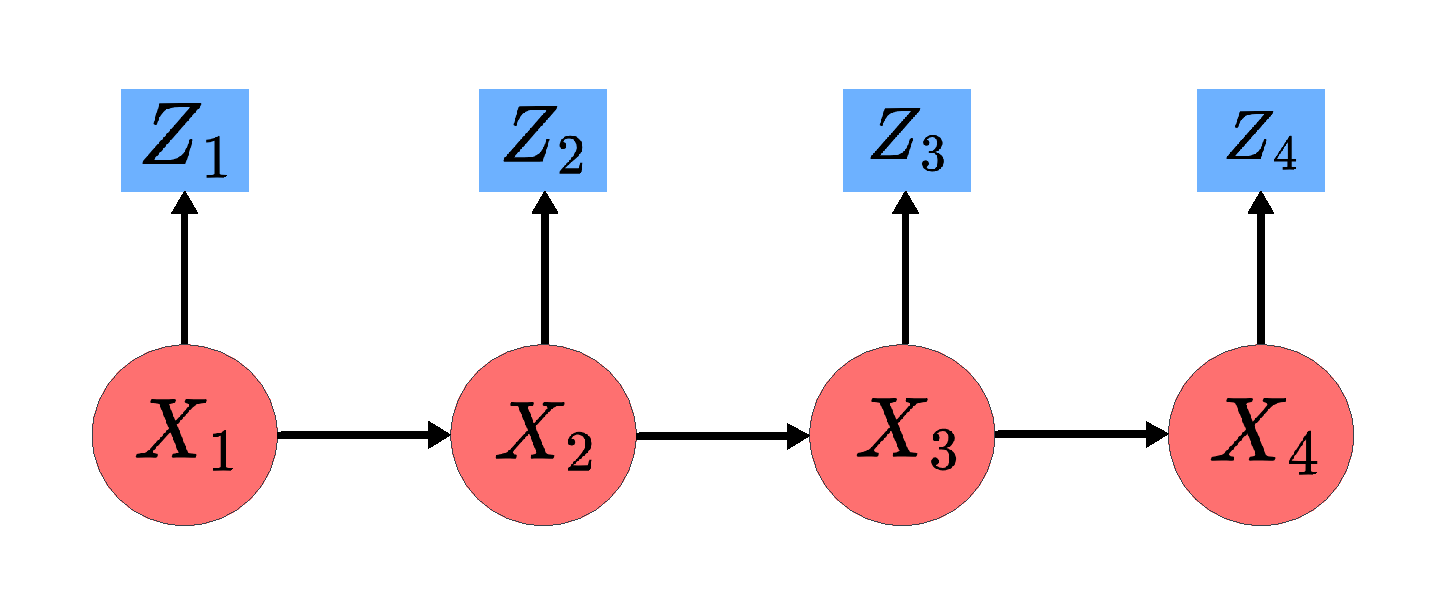
\includegraphics[width=0.5\linewidth]{img/BeyseNetAppendix}
	\caption{شبکه بیز معادل مربوط به مسئله مثال  تخمین حالت بیان‌شده}
	\label{fig:beysenetappendix}
\end{figure}

فرمول‌بندی احتمالاتی بیزی که تا کنون ذکر شده است، می‌تواند به صورت گرافیکی
با استفاده از شبکه‌های بیزی ارائه شود. یک شبکه بیزی
\footnote{\lr{BayesNet}}
یک مدل گرافیکی جهت‌دار است
که متغیرهای تصادفی به عنوان گره‌های آن و یال‌ها نمایانگر وابستگی‌ها (علت و معلول)
بین این گره‌ها هستند. به عبارت دیگر، یک شبکه بیزی می‌تواند توزیع احتمالی مشترک
را بر روی همه متغیرهای تصادفی به عنوان حاصل‌ضرب چگالی‌های شرطی تعریف کند. شکل~\ref{fig:beysenetappendix}
شبکه بیزی مربوط به سیستم غیرخطی مثال ما را نشان می‌دهد. توزیع احتمالی مشترک
مربوطه ممکن است به صورت زیر نوشته شود:
\begin{equation} \label{eq:JointProbability_Distribution}
	p(X, Z) = p(x_1) p(x_2|x_1) p(x_3|x_2) p(x_4|x_3) \newline
	\times p(z_1|x_1) p(z_2|x_2) p(z_3|x_3) p(z_4|x_4)
\end{equation}
در این معادله، تکه اول اول نمایانگر مدل سیستم و تکه دوم
نمایانگر مدل‌های مشاهده است.

 توزیع مشترک در معادله
 \ref{eq:MAP}
 به توزیع پسین \(p(X|Z)\) با استفاده از فرمول احتمال شرطی زیر پیوند می‌خورد:
\begin{equation}
	p(X|Z) = \frac{p(X, Z)}{p(Z)}
\end{equation}
\(p(Z)\) در این معادله به عنوان یک عامل نرمال‌سازی عمل می‌کند، بنابراین \(p(X|Z)\) متناسب با توزیع مشترک \(p(Z, X)\) است. تخمین $MAP$ معادل خواهد بود با بیشینه‌سازی تابع درست‌نمایی \(l(X; Z)\) که متناسب با \(p(Z, X)\) است:
\begin{equation}
	l(X; Z) \propto p(Z|X)
\end{equation}
بدین‌ترتیب خواهیم داشت:
\begin{equation}
	X^{MAP} = \arg\max_X l(X; Z)
\end{equation}
علاوه بر این، می‌توانیم مقیاس‌های ثابت را در احتمالات شرطی معادلات
\ref{eq:Gauess_Dis_h}
و
\ref{eq:Gauess_Dis_F}
حذف کنیم و تابع درست‌نمایی \(l(X; Z)\) را به صورت زیر بنویسیم:
\begin{equation} \label{eq:Likelihood}
	l(X; Z) = l(x_1) l(x_2|x_1) l(x_3|x_2) p(x_4|x_3) \\
	\times l(z_1|x_1) l(z_2|x_2) l(z_3|x_3) l(z_4|x_4)
\end{equation}
که در آن:
\begin{equation}
	l(X; z) = \exp \left\{ -\frac{1}{2} \|g(X) - z \|_R^2 \right\}
\end{equation}
\begin{equation}
	l(X_{k+1}; X_k) = \exp \left\{ -\frac{1}{2} \|f(X_k, u_k) - X_{k+1}\|_Q^2 \right\}
\end{equation}

\begin{figure} [!t]
	\centering
	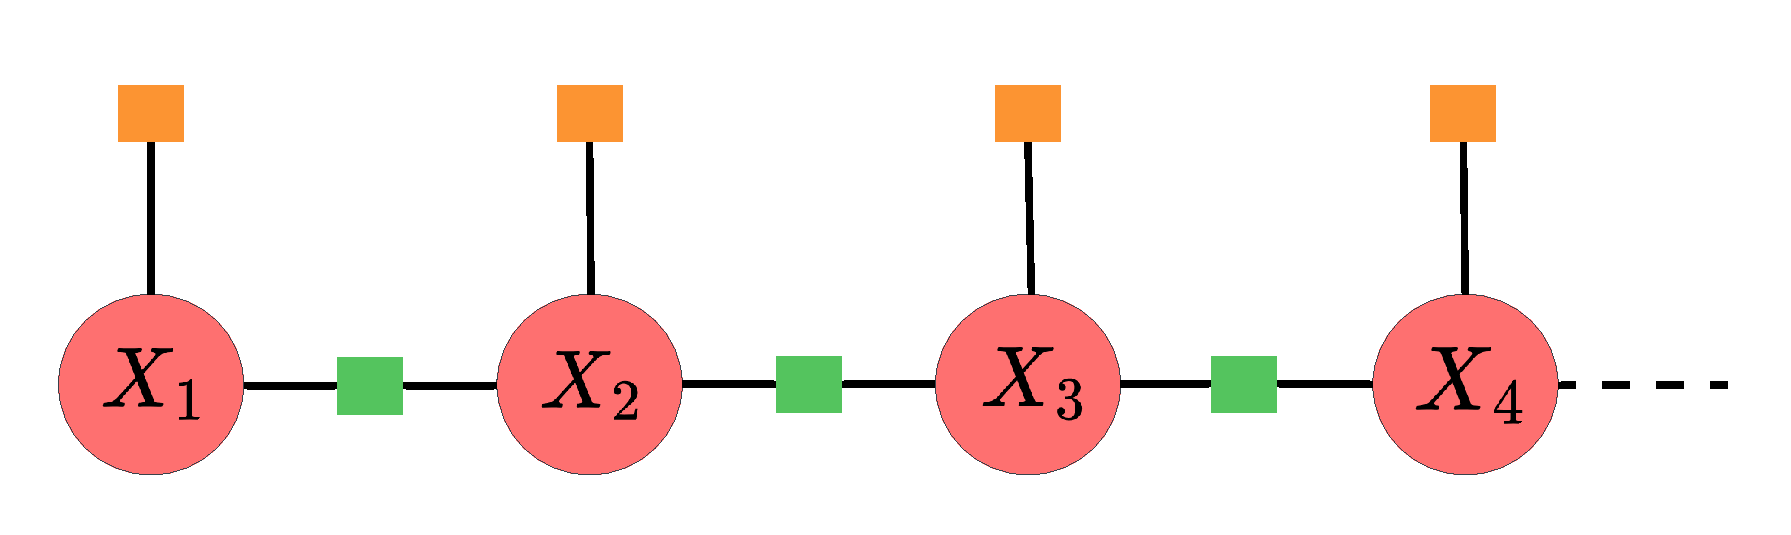
\includegraphics[width=0.6\linewidth]{img/StateEstimationFGAppendinx}
	\caption{گراف عامل معادل مربوط به مسئله مثال  تخمین حالت بیان‌شده}
	\label{fig:stateestimationfgappendinx}
\end{figure}

بنابراین، تابع درست‌نمایی که باید بیشینه شود، حاصل‌ضرب تجزیه‌شده‌ای از توابع درست‌نمایی کوچکتر است. در حالی که توزیع احتمالی مشترک در معادله
\ref{eq:JointProbability_Distribution}
به بهترین شکل با استفاده از یک شبکه بیزی توصیف می‌شود، تابع درست‌نمایی تجزیه‌شده در معادله
\ref{eq:Likelihood}
می‌تواند به بهترین شکل با یک گراف عامل نمایش داده شود.

یک گراف عامل \(G\) تجزیه یک تابع \(f(X)\) را به عنوان حاصل‌ضربی از عامل‌های \(f_i\) تعریف می‌کند. این یک مدل گرافیکی دو بخشی و بدون جهت با دو نوع گره است: گره‌های عامل \(f_i \in F\) و گره‌های متغیر \(x_i \in X\). یک یال \(e_{ij} \in E\) در گراف حضور دارد اگر و فقط اگر \(f_i\) تابعی از \(x_j\) باشد
\cite{kaess2012concurrent}. 
شکل
\ref{fig:stateestimationfgappendinx}
گراف عامل متناظر با تابع درست‌نمایی در معادله
\ref{eq:Likelihood}
را نشان می‌دهد. در این شکل، عامل‌های آبی رنگ به درست‌نمایی‌های اندازه‌گیری اشاره دارند در حالی که عامل‌های سبز رنگ به مدل سیستم اشاره می‌کنند.
در نهایت، با استفاده از الگوریتم $ML$، مسئله $MAP$ به یک مسئله $LS$ غیرخطی زیر تبدیل می‌شود:
\begin{equation}
	X^{MAP} = \arg\max_X l(X; Z) = \arg\max_X \text{Ln}\left(\prod_i l_i (X_i; Z_i)\right)
\end{equation}
\begin{equation}
    X^{MAP}	= \arg\min_X \left(\sum_{i=0}^k \left(\|f(x_i, u_i) - x_{i+1}\|_{Q_i}^2 + \|h(x_i) - z_i\|_{R_i}^2\right)\right)
\end{equation}

در مورد سیستم‌های ناوبری، \(X\) نشان‌دهنده مکان‌های پیگیری شده است که از طریق عامل‌های مدل حرکت به یکدیگر متصل می‌شوند. از طرف دیگر، هر حالت نیز با فاکتورهای مدل اندازه‌گیری محدود می‌شود.

\section{حل‌کننده‌ها}

راه‌حل یک مسئله $LS$ که به یک گراف عامل مربوط است، می‌تواند به چهار روش تقسیم شود. در ادامه، این چهار روش معرفی می‌شوند.

\textbf{بهینه‌سازهای دسته‌ای}

در بهینه‌سازی دسته‌ای، همه عامل‌ها از ابتدای زمان تا لحظه فعلی در الگوریتم بهینه‌سازی شرکت می‌کنند. از آنجا که تمام اطلاعات در مسئله بهینه‌سازی شرکت می‌کنند، این روش دقیق‌ترین نتیجه را به دست می‌دهد. با این حال، به دلیل بار محاسباتی سنگین، این یک الگوریتم آفلاین است.

\textbf{فیلترها و صاف‌کننده‌های با تأخیر ثابت}

بهینه‌سازهای دسته‌ای با گذشت زمان در پیچیدگی رشد می‌کنند، بنابراین اجرای آن‌ها در زمان واقعی غیرممکن خواهد بود. بنابراین، یک راه‌حل این است که اطلاعات قدیمی را با حاشیه‌نویسی حذف کنیم و اثر تجمعی آن‌ها را به عنوان یک عامل پیشین در انتهای گراف عامل بریده‌شده اضافه کنیم. این حاشیه‌نویسی و برش در هر تکرار الگوریتم رخ می‌دهد. مقیاس مسئله در این حالت ثابت می‌ماند و به اندازه پنجره بستگی دارد.

در فیلتر کردن، که یک حالت شدید از صاف کردن با تأخیر ثابت است، همه داده‌های قبلی تا گره فعلی به یک عامل پیشین واحد فشرده می‌شوند. این حالت کمترین سربار محاسباتی و ذخیره‌سازی را دارد. اگرچه این برش گراف عامل برای سیستم‌های خطی هیچ اثر تباه‌کننده‌ای ندارد، اما برای سیستم‌های غیرخطی، منجر به تجمع خطاها در عامل پیشین می‌شود. این تجمع به دلیل اصلاح نقاط خطی‌سازی در هر تکرار است که دیگر نمی‌توانند به گره‌های قبلی منتقل شوند.

\textbf{صاف‌کننده‌های افزایشی}

صاف کردن افزایشی که در
\cite{kaess2012concurrent}
ارائه شده است، یک الگوریتم جدید برای افزودن افزایشی و حل گراف عامل به صورت افزایشی با ورود داده‌های جدید است. از آنجا که مسائل تخمین حالت در رباتیک معمولاً به یک زنجیره مارکوف منجر می‌شوند، گراف فاکتور تولید شده اغلب تنک است و تجزیه ماتریس مورد نیاز در طی اجرای بهینه‌سازی غیرخطی تکراری می‌تواند به صورت کارآمدتری انجام شود. نویسندگان در
\cite{kaess2012concurrent}
از روش‌های تجزیه ماتریس تکراری برای توسعه الگوریتم خود بهره‌برداری می‌کنند.

به دلیل ماهیت مارکوفی مسئله، شبکه بیزی تولید شده یک گراف وتری
\footnote{\lr{chordal graph}}
 است. این گراف وتری سپس به یک درخت بیزی تبدیل می‌شود. ممکن است اطلاعات جدید به‌راحتی اضافه شوند بدون نیاز به اجرای مجدد تمام محاسبات. با اینکه زمان محاسباتی این روش بسیار کمتر است، نیازهای حافظه تغییر نمی‌کنند. علاوه بر این، نمی‌توان مطمئن بود که هر تکرار از این الگوریتم چقدر زمان خواهد برد. بنابراین، به‌طور کلی، این روش نمی‌تواند تخمین‌های قطعی ارائه دهد، و بر اساس مسئله و اندازه‌گیری‌های مشاهده‌شده، زمان محاسباتی ممکن است به‌طور قابل‌توجهی متفاوت باشد. به عنوان مثال، وقتی یک محدودیت حلقه اضافه می‌کنیم، تکرار جدید نیاز دارد تا بخش بیشتری از درخت پردازش شود، که نیازمند زمان محاسباتی بسیار بیشتری است.

\textbf{فیلتر کردن و صاف کردن همزمان}

مقاله
\cite{kaess2012concurrent}
یک چارچوب با یک فیلتر در حال اجرا در کنار یک صاف‌کننده ارائه می‌دهد. در هر تکرار صاف‌کننده، فیلتر می‌تواند چندین بار تکرار شود و تخمین‌های بلادرنگ ارائه دهد. سپس، در انتهای هر تکرار صاف‌کننده، این دو سیستم هماهنگ می‌شوند. جداسازی این دو سیستم از طریق یک متغیر جداکننده میانی در درخت بیزی به دست می‌آید. با داشتن این متغیر، فیلتر از لحاظ آماری از صاف‌کننده مستقل خواهد بود. در مرحله همگام‌سازی، جداکننده به‌روزرسانی می‌شود به طوری که حالت‌های جدیداً اضافه‌شده به فیلتر به درخت صاف‌کننده منتقل شوند.

\section{کتابخانه GTSAM}

همان‌طور که در بخش‌های قبلی ذکر شد، گراف‌های عامل ابزارهای قدرتمندی برای فرمول‌بندی مسائل تخمین حالت و کالیبراسیون هستند. به دلیل انعطاف‌پذیری آن‌ها، این گراف‌ها به روشی کارآمد برای ساخت مسائل بهینه‌سازی نقشه در سیستم‌های SLAM تبدیل شده‌اند. بنابراین، بسیاری از
حل‌کننده‌های متن‌باز و کارآمد برای پیاده‌سازی این ابزار توسعه داده شده‌اند. یکی از کتابخانه‌های
مهم، GTSAM 
\cite{gtsam}
است. این کتابخانه در دانشگاه جورجیاتک توسعه یافته و یک رابط برنامه‌نویسی کامل برای پیاده‌سازی عامل‌های سفارشی، تعریف گراف‌های عامل، و حل آن‌ها به‌صورت کارآمد فراهم می‌کند.

علاوه بر این، GTSAM از بهینه‌سازی روی منیفلدها نیز پشتیبانی می‌کند، که در مواردی که با مسائل بهینه‌سازی مواجه هستیم که به پارامترهایی از گروه‌های اقلیدسی خاص مربوط می‌شوند، ضروری است. این کتابخانه همچنین یک رابط نرم‌افزار متلب برای توسعه سریع ارائه می‌دهد. در نهایت، بسیاری از عامل‌ها که قبلاً در این کتابخانه پیاده‌سازی شده‌اند، آماده بهره‌برداری برای مسائل رباتیک و SLAM هستند.		% پیوست اول: آشنایی مقدماتی با لاتک
%\chapter{‌جدول، نمودار و الگوریتم در لاتک}
		% پیوست دوم: جدول، نمودار و الگوریتم در لاتک
%\chapter{مراجع، واژه‌نامه و حاشیه‌نویسی}
   	% پیوست سوم: مراجع، واژه‌نامه و حاشیه‌نویسی

\onehalfspacing
\cleardoublepage
% برگرداندن شماره‌بندی صفحات فصول
\let\chapter\Chapter
\pagenumbering{tartibi} % اول، دوم، ...
\baselineskip=.75cm

% چاپ واژه‌نامه‌ها و نمایه: در صورتی که نمی‌خواهید واژه‌نامه‌ها و نمایه نمایش داده شوند سه خط زیر را کامنت نمایید.
%\printglossary
%\cleardoublepage
%\printindex

\begin{latin}
\baselineskip=.6cm
\latinabstract
\latinTitlePage
\end{latin}
\label{LastPage}

\end{document}
